\documentclass[10pt]{article}
\usepackage[english]{babel}
\usepackage[utf8]{inputenc}

% includes references in the table of contents
\usepackage[nottoc]{tocbibind}

\usepackage{amsthm}
\theoremstyle{plain}
\usepackage{thmtools}
\usepackage{enumerate}
\newtheorem{theorem}{Theorem}

\theoremstyle{definition}
\newtheorem{definition}[theorem]{Definition}

\usepackage{algorithm}
\usepackage{algpseudocode}

\usepackage{booktabs}
\usepackage{hyperref}
\usepackage{amsmath}
\usepackage{amssymb}
\usepackage{graphicx}
\usepackage{subcaption}
\usepackage{fancyhdr}
\usepackage{vmargin}
\setmarginsrb{2cm}  % left margin
             {2cm}  % top margin
             {2cm}  % right margin
             {2cm}  % bottom margin
             {1.5cm}  % head height
             {1cm}  % head sep
             {1.5cm}  % foot height
             {1cm}  % foot sep
   
\title{Support Vector Machines}
\author{Donato Meoli}
\date{April, 2021}

\makeatletter
\let\thetitle\@title
\let\theauthor\@author
\let\thedate\@date

\newcommand{\algorithmicbreak}{\textbf{break}}
\newcommand{\Break}{\State \algorithmicbreak}

\algnewcommand\AND{\textbf{and }}
\algnewcommand\OR{\textbf{or }}
\algnewcommand\NOT{\textbf{not }}

% Algorithmic modifications
\newenvironment{breakablealgorithm}
  {% \begin{breakablealgorithm}
   \begin{center}
     \refstepcounter{algorithm}% New algorithm
     \hrule height.8pt depth0pt \kern2pt% \@fs@pre for \@fs@ruled
     \renewcommand{\caption}[2][\relax]{% Make a new \caption
       {\raggedright\textbf{\fname@algorithm~\thealgorithm} ##2\par}%
       \ifx\relax##1\relax % #1 is \relax
         \addcontentsline{loa}{algorithm}{\protect\numberline{\thealgorithm}##2}%
       \else % #1 is not \relax
         \addcontentsline{loa}{algorithm}{\protect\numberline{\thealgorithm}##1}%
       \fi
       \kern2pt\hrule\kern2pt
     }
  }{% \end{breakablealgorithm}
     \kern2pt\hrule\relax% \@fs@post for \@fs@ruled
   \end{center}
  }
\makeatother

\pagestyle{fancy}
\fancyhf{}
\rhead{\thepage}
\lhead{\thetitle}
\cfoot{}

\begin{document}

\begin{titlepage}
	\centering
    \vspace*{0.5 cm}
    \includegraphics[scale=0.5]{img/unipi}\\[1.0 cm]
    \textsc{\LARGE University of Pisa}\\[0.5 cm]
    \textsc{\Large Department of Computer Science}\\[1.5 cm]
	\textsc{\large Computational Mathematics \\ Wildcard Project nr. 5 with Machine Learning \\ Group 35}\\[0.5 cm]
	\rule{\linewidth}{0.2 mm} \\[0.4 cm]
	{ \huge \bfseries \thetitle}\\
	\rule{\linewidth}{0.2 mm} \\[1.5 cm]
	\centering \textsc{\large \emph{Author:}}\\[0.5 cm]
	\begin{minipage}{0.4\textwidth}
		\begin{center} \large
			\textbf{\theauthor}
			\texttt{\href{mailto::d.meoli@studenti.unipi.it}{d.meoli@studenti.unipi.it}}
		\end{center}
		\end{minipage}~
		\begin{minipage}{0.4\textwidth}
	\end{minipage}\\[2 cm]
	{\large \thedate}\\[2 cm]
	\vfill
\end{titlepage}

\tableofcontents

\pagebreak

\listoffigures

\pagebreak

\listoftables

\pagebreak

\listofalgorithms
\addcontentsline{toc}{section}{List of Algorithms}

\pagebreak

\listoftheorems

\pagebreak

\section{Track}

\begin{itemize}
\item[\texttt{(M1.1)}] is a \emph{Support Vector Classifier (SVC)} with the \emph{hinge} loss.

\begin{itemize}
\item[\texttt{(A1.1.1)}] is a \emph{momentum descent} approach~\cite{polyak1964some, nesterov1998introductory, nesterov1983method}, an \emph{accelerated gradient} method for solving the SVC in its \emph{primal} formulation.

\item[\texttt{(A1.1.2)}] is the \emph{Sequential Minimal Optimization (SMO)} algorithm~\cite{platt1998sequential, keerthi2001improvements}, an ad hoc \emph{active set} method for training a SVC in its \emph{Wolfe dual} formulation with \emph{linear}, \emph{polynomial} and \emph{gaussian} kernels.

\item[\texttt{(A1.1.3)}] is the \emph{AdaGrad} algorithm~\cite{duchi2011adaptive}, a \emph{deflected subgradient} method for solving the SVC in its \emph{Lagrangian dual} formulation with \emph{linear}, \emph{polynomial} and \emph{gaussian} kernels.
\end{itemize}

\end{itemize}

\begin{itemize}
\item[\texttt{(M1.2)}] is a \emph{Support Vector Classifier (SVC)} with the \emph{squared hinge} loss.

\begin{itemize}
\item[\texttt{(A1.2.1)}] is a \emph{momentum descent} approach~\cite{polyak1964some, nesterov1998introductory, nesterov1983method}, an \emph{accelerated gradient} method for solving the SVC in its \emph{primal} formulation.
\end{itemize}

\end{itemize}

\bigskip

\begin{itemize}
\item[\texttt{(M2.1)}] is a \emph{Support Vector Regression (SVR)} with the \emph{epsilon-insensitive} loss.

\begin{itemize}
\item[\texttt{(A2.1.1)}] is a \emph{momentum descent} approach~\cite{polyak1964some, nesterov1998introductory, nesterov1983method}, an \emph{accelerated gradient} method for solving the SVR in its \emph{primal} formulation.

\item[\texttt{(A2.1.2)}] is the \emph{Sequential Minimal Optimization (SMO)} algorithm~\cite{flake2002efficient, shevade1999improvements}, an ad hoc \emph{active set} method for training a SVR in its \emph{Wolfe dual} formulation with \emph{linear}, \emph{polynomial} and \emph{gaussian} kernels.

\item[\texttt{(A2.1.3)}] is the \emph{AdaGrad} algorithm~\cite{duchi2011adaptive}, a \emph{deflected subgradient} method for solving the SVR in its \emph{Lagrangian dual} formulation with \emph{linear}, \emph{polynomial} and \emph{gaussian} kernels.
\end{itemize}

\end{itemize}

\begin{itemize}
\item[\texttt{(M2.2)}] is a \emph{Support Vector Regression (SVR)} with the \emph{squared epsilon-insensitive} loss.

\begin{itemize}
\item[\texttt{(A2.2.1)}] is a \emph{momentum descent} approach~\cite{polyak1964some, nesterov1998introductory, nesterov1983method}, an \emph{accelerated gradient} method for solving the SVR in its \emph{primal} formulation.
\end{itemize}

\end{itemize}
\section{Abstract}

A \emph{Support Vector Machine} is a learning model used both for \emph{classification} and \emph{regression} tasks whose goal is to construct a \emph{maximum margin separator}, i.e., a decision boundary with the largest distance from the nearest training data points.

The aim of this report is to compare the \emph{primal}, the \emph{Wolfe dual}~\cite{fletcher2009support} and the \emph{Lagrangian dual} formulations of this model in terms of \emph{complexity}.

Firstly, a detailed mathematical derivation of the model for all these formulations is given, then three algorithms are described to solve the optimization problem in case of \emph{primal}, \emph{Wolfe dual} or \emph{Lagrangian dual} formulation of the problem, explaining their theoretical properties, i.e., \emph{convergence rate} and \emph{complexity}.

Finally, some experiments are shown for \emph{linearly} and \emph{nonlinearly} separable generated datasets to compare the performance with different \emph{hyperparameters} and different \emph{kernels}, also comparing the \emph{custom} results with \emph{sklearn}'s SVM implementations, i.e., \emph{liblinear}~\cite{fan2008liblinear} and \emph{libsvm}~\cite{chang2011libsvm} implementations, and the \emph{cvxopt}~\cite{vandenberghe2010cvxopt} QP solver.

\pagebreak

\section{Linear Support Vector Classifier} \label{section:svc}

Given $n$ training points, where each input $x_i$ has $m$ attributes, i.e., is of dimensionality $m$, and is in one of two classes $y_i=\pm1$, i.e., our training data is of the form:

\begin{equation}
	\{(x_i,y_i), x_i\in\Re^m, y_i=\pm1, i=1, \dots, n\} \label{eq:svc_data}
\end{equation}

For simplicity we first assume that data are (not fully) linearly separable in the input space $x$, meaning that we can draw a line separating the two classes when $m=2$, a plane for $m=3$ and, more in general, a hyperplane for an arbitrary $m$.

Support vectors are the examples closest to the separating hyperplane and the aim of support vector machines is to orientate this hyperplane in such a way as to be as far as possible from the closest members of both classes, i.e., we need to maximize this margin.

This hyperplane is represented by the equation $w^T x + b=0$. So, we need to find $w$ and $b$ so that our training data can be described by:

\begin{equation} \label{eq:svc_consts}
	\begin{aligned}
		& w^T x_i + b \geq +1 - \xi_i, \forall y_i=+1 \\
    	& w^T x_i + b \leq -1 + \xi_i, \forall y_i=-1 \\
    	& \xi_i \geq 0 \ \forall_i
	\end{aligned}
\end{equation}

where the positive slack variables $\xi_i$ are introduced to allow misclassified points. In this way data points on the incorrect side of the margin boundary will have a penalty that increases with the distance from it.

These two equations can be combined into:

\begin{equation} \label{eq:svc_const}
	\begin{aligned}
    	& y_i (w^T x_i + b) \geq 1 - \xi_i \ \forall_i \\
    	& \xi_i\geq 0 \ \forall_i
    \end{aligned}
\end{equation}

The margin is equal to $\displaystyle \frac{1}{\| w \|}$ and maximizing it subject to the constraint in~\eqref{eq:svc_const} while as we are trying to reduce the number of misclassifications is equivalent to finding:

\begin{equation} \label{eq:svc_obj}
    \begin{aligned}
        \min_{w,b,\xi} \quad & \| w \| + C \sum_{i=1}^n \xi_i \\
            \text{subject to} \quad & y_i (w^T x_i + b) \geq 1 - \xi_i \ \forall_i \\ & \xi_i \geq 0 \ \forall_i
    \end{aligned}
\end{equation}

Minimizing $\| w \|$ is equivalent to minimizing $\displaystyle \frac{1}{2} \| w \|^2$, but in this form we will deal with a 1-strongly convex regularization term that has more desirable convergence properties. So we need to find:

\begin{equation} \label{eq:quad_svc_obj}
    \begin{aligned}
        \min_{w,b,\xi} \quad & \frac{1}{2} \| w \|^2 + C \sum_{i=1}^n \xi_i \\
            \text{subject to} \quad & y_i (w^T x_i + b) \geq 1 - \xi_i \ \forall_i \\ & \xi_i \geq 0 \ \forall_i
    \end{aligned}
\end{equation}

where the parameter $C$ controls the trade-off between the slack variable penalty and the size of the margin.

\begin{figure}[h!]
	\centering
	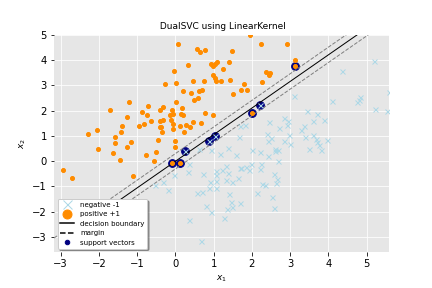
\includegraphics[scale=0.6]{img/linear_dual_l1_svc_hyperplane}
	\caption{Linear SVC hyperplane}
	\label{fig:linear_dual_l1_svc_hyperplane}
\end{figure}

\pagebreak

\subsection{Hinge loss}

The \emph{hinge} loss is defined as:

\begin{equation} \label{eq:hinge_loss1}
	\mathcal{L}_1 = \max(0, 1 - y (w^T x + b))
\end{equation}

or, equivalently:

\begin{equation} \label{eq:hinge_loss2}
	\mathcal{L}_1 = 
	\begin{cases}
		0 & \text{if} \ y (w^T x + b) \geq 1 \\
		1 - y (w^T x + b) & \text{otherwise} \\
	\end{cases}
\end{equation}

and it is a nondifferentiable convex function due to its nonsmoothness in 1, but has a subgradient that is given by:

\begin{equation} \label{eq:hinge_loss_der}
    \partial_w \mathcal{L}_1=
        \begin{cases}
            -y x & \text{if} \ y (w^T x + b) < 1 \\
            0 & \text{otherwise} \\ 
        \end{cases}
\end{equation}

\subsubsection{Primal formulation}

The general primal unconstrained formulation takes the form:

\begin{equation} \label{eq:primal_svm}
    \min_{w,b} \frac{1}{2} \| w \|^2 + C \sum_{i=1}^n \mathcal{L}(w,b;x_i,y_i)
\end{equation}

where $\displaystyle \frac{1}{2} \| w \|^2$ is the \emph{regularization term} and $\mathcal{L}(w,b;x_i,y_i)$ is the \emph{loss function} associated with the observation $(x_i,y_i)$~\cite{piccialli2018nonlinear}.

The quadratic optimization problem~\eqref{eq:quad_svc_obj} can be equivalently formulated as:

\begin{equation} \label{eq:primal_l1_svc}
    \min_{w,b} \frac{1}{2} \| w \|^2 + C \sum_{i=1}^n \max(0, 1 - y_i (w^T x_i + b))
\end{equation}

where we make use of the \emph{hinge} loss~\eqref{eq:hinge_loss1} or~\eqref{eq:hinge_loss2}.

The above formulation penalizes slacks $\xi$ linearly and is called $\mathcal{L}_1$-SVC.

\begin{figure}[h!]
	\centering
  	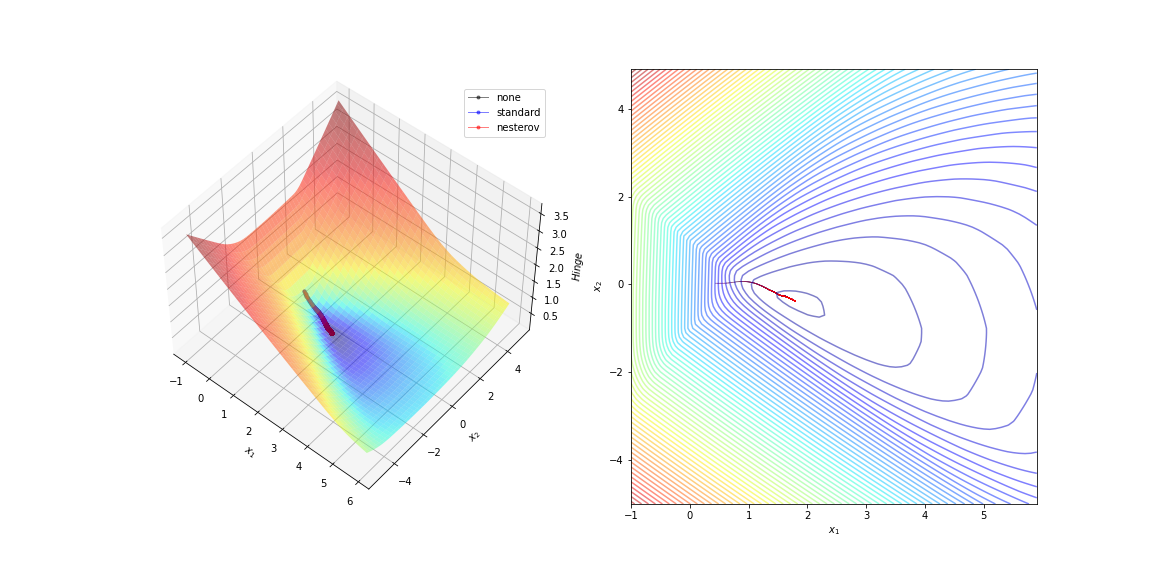
\includegraphics[scale=0.4]{img/l1_svc_loss}
  	\caption{Hinge loss with different optimization steps}
  	\label{fig:l1_svc_loss}
\end{figure}

To simplify the notation and so also the design of the algorithms, the simplest approach to learn the bias term $b$ is that of including that into the \emph{regularization term}; so we can rewrite~\eqref{eq:primal_svm} as follows:

\begin{equation} \label{eq:reg_bias_primal_svm1}
    \min_{w,b} \frac{1}{2} (\| w \|^2 + b^2) + C \sum_{i=1}^n \mathcal{L}(w,b;x_i,y_i)
\end{equation}

or, equivalently, by augmenting the weight vector $w$ with the bias term $b$ and each instance $x_i$ with an additional dimension, i.e., with constant value equal to 1:

\begin{equation} \label{eq:reg_bias_primal_svm2}
    \begin{aligned}
        \min_{w} \quad & \frac{1}{2} \| \hat{w} \|^2 + C \sum_{i=1}^n \mathcal{L}(\hat{w};\hat{x}_i,y_i) \\
            \text{where} \quad & \hat{w}^T = [w^T, b] \\ & \hat{x}_i^T = [x_i^T, 1]
    \end{aligned}
\end{equation}

with the advantages of having convex properties of the objective function useful for convergence analysis and the possibility to directly apply algorithms designed for models without the bias term.

In the specific case of the $\mathcal{L}_1$-SVC the objective~\eqref{eq:primal_l1_svc} become:

\begin{equation} \label{eq:reg_bias_primal_l1_svc}
    \min_{w,b} \frac{1}{2} (\| w \|^2 + b^2) + C \sum_{i=1}^n \max(0, 1 - y_i (w^T x_i + b))
\end{equation}

Note that in terms of numerical optimization the formulation~\eqref{eq:primal_l1_svc} is not equivalent to~\eqref{eq:reg_bias_primal_l1_svc} since in the first one the bias term $b$ does not contribute to the \emph{regularization term}, so the SVM formulation is based on an unregularized bias term $b$, as highlighted by the \emph{statistical learning theory}. But, in machine learning sense, numerical experiments in~\cite{hsu2002simple} show that the accuracy does not vary much when the bias term $b$ is embedded into the weight vector $w$.

\subsubsection{Wolfe Dual formulation}

To reformulate the~\eqref{eq:quad_svc_obj} as a \emph{Wolfe dual}, we need to allocate the Lagrange multipliers $\alpha_i, \mu_i \geq 0 \ \forall_i$:

\begin{equation} \label{eq:svc_wolfe_dual}
    \max_{\alpha,\mu} \min_{w,b,\xi} \mathcal{W}(w,b,\xi,\alpha,\mu) = \frac{1}{2} \| w \|^2 + C \sum_{i=1}^n \xi_i-\sum_{i=1}^n \alpha_i(y_i(w^T x_i + b)-1+\xi_i)-\sum_{i=1}^n\mu_i\xi_i
\end{equation}

We wish to find the $w$, $b$ and $\xi_i$ which minimizes, and the $\alpha$ and $\mu$ which maximizes $\mathcal{W}$, provided $\alpha_i\geq 0, \mu_i \geq 0 \ \forall_i$. We can do this by differentiating $\mathcal{W}$ wrt $w$ and $b$ and setting the derivatives to 0:

\begin{equation} \label{eq:svc_wolfe_der_w}
	\frac{\partial \mathcal{W}}{\partial w}=w-\sum_{i=1}^n \alpha_i y_i x_i \Rightarrow w=\sum_{i=1}^n \alpha_i y_i x_i
\end{equation}

\begin{equation} \label{eq:svc_wolfe_der_b}
	\frac{\partial \mathcal{W}}{\partial b}=-\sum_{i=1}^n \alpha_i y_i\Rightarrow\sum_{i=1}^n \alpha_i y_i=0
\end{equation}

\begin{equation} \label{eq:svc_wolfe_der_xi}
	\frac{\partial \mathcal{W}}{\partial\xi_i}=0\Rightarrow C=\alpha_i+\mu_i
\end{equation}

Substituting~\eqref{eq:svc_wolfe_der_w} and~\eqref{eq:svc_wolfe_der_b} into~\eqref{eq:svc_wolfe_dual} together with $\mu_i\geq 0 \ \forall_i$, which implies that $\alpha\leq C$, gives a new formulation being dependent on $\alpha$. We therefore need to find:

\begin{equation} \label{eq:svc_max_wolfe_dual}
	\begin{aligned}
    	\max_{\alpha} \mathcal{W}(\alpha) &= \sum_{i=1}^n \alpha_i - \frac{1}{2}\sum_{i,j}\alpha_i\alpha_j y_i y_j \langle x_i, x_j \rangle \\
    	&= \sum_{i=1}^n \alpha_i - \frac{1}{2}\sum_{i,j}\alpha_i Q_{ij}\alpha_j \ \text{where} \ Q_{ij} = y_i y_j \langle x_i, x_j \rangle \\
    	&= \sum_{i=1}^n \alpha_i - \frac{1}{2}\alpha^T Q\alpha \ \text{subject to} \ 0\leq\alpha_i\leq C \ \forall_i, \sum_{i=1}^n \alpha_i y_i=0 
	\end{aligned}
\end{equation}

or, equivalently:

\begin{equation} \label{eq:svc_min_wolfe_dual}
    \begin{aligned}
        \min_{\alpha} \quad & \frac{1}{2}\alpha^T Q\alpha+q^T\alpha \\
            \text{subject to} \quad & 0\leq\alpha_i\leq C \ \forall_i \\ & y^T\alpha=0
    \end{aligned}
\end{equation}

where $q^T = [1, \dots, 1]$.

By solving~\eqref{eq:svc_min_wolfe_dual} we will know $\alpha$ and, from~\eqref{eq:svc_wolfe_der_w}, we will get $w$, so we need to calculate $b$.

We know that any data point satisfying~\eqref{eq:svc_wolfe_der_b} which is a support vector $x_s$ will have the form:

\begin{equation} \label{eq:svc_sv_const1}
	y_s(w^T x_s + b)=1
\end{equation}

and, by substituting in~\eqref{eq:svc_wolfe_der_w}, we get:

\begin{equation} \label{eq:svc_sv_const2}
	y_s\big(\sum_{m\in S}\alpha_m y_m \langle x_m, x_s \rangle +b\big)=1
\end{equation}

where $s$ denotes the set of indices of the support vectors and is determined by finding the indices $i$ where $\alpha_i>0$, i.e., nonzero Lagrange multipliers.

Multiplying through by $y_s$ and then using $y_s^2=1$ from~\eqref{eq:svc_consts}:

\begin{equation} \label{eq:svc_sv_squared_const2}
	y_s^2\big(\sum_{m\in S}\alpha_m y_m \langle x_m, x_s \rangle +b\big)=y_s
\end{equation}

\begin{equation} \label{eq:svc_b}
	b=y_s-\sum_{m\in S}\alpha_m y_m \langle x_m, x_s \rangle
\end{equation}

Instead of using an arbitrary support vector $x_s$, it is better to take an average over all of the support vectors in $S$:

\begin{equation} \label{eq:svc_b_avg}
	b=\frac{1}{N_s}\sum_{s\in S} y_s-\sum_{m\in S}\alpha_m y_m \langle x_m, x_s \rangle
\end{equation}

We now have the variables $w$ and $b$ that define our separating hyperplane's optimal orientation and hence our support vector machine. Each new point $x'$ is classified by evaluating:

\begin{equation} \label{eq:svc_pred}
    y'=\operatorname{sign}\big(\sum_{i=1}^n\alpha_i y_i\langle x_i, x' \rangle+b\big)
\end{equation}

From~\eqref{eq:svc_min_wolfe_dual} we can notice that the equality constraint $y^T \alpha = 0$ arises form the stationarity condition $\partial_{{b}} \mathcal{W}=0$. So, again, for simplicity, we can again consider the bias term $b$ embedded into the weight vector. We report below the box-constrained dual formulation~\cite{hsu2002simple} that arises from the primal~\eqref{eq:reg_bias_primal_svm1} or~\eqref{eq:reg_bias_primal_svm2} where the bias term $b$ is embedded into the weight vector $w$:

\begin{equation} \label{eq:svc_min_bcqp_wolf_dual}
    \begin{aligned}
        \min_{\alpha} \quad & \frac{1}{2} \alpha^T (Q + yy^T)\alpha+q^T\alpha \\
            \text{subject to} \quad & 0\leq\alpha_i\leq C \ \forall_i
    \end{aligned}
\end{equation}

\subsubsection{Lagrangian Dual formulation}

In order to relax the constraints in the \emph{Wolfe dual} formulation~\eqref{eq:svc_min_wolfe_dual} we define the problem as a \emph{Lagrangian dual} relaxation by embedding them into objective function, so we need to allocate the Lagrange multipliers $\mu$ and $\lambda_+, \lambda_- \geq 0$:

\begin{equation} \label{eq:svc_lagrangian_dual}
	\begin{aligned}
		    \max_{\mu,\lambda_+,\lambda_-} \min_{\alpha} \mathcal{L}(\alpha,\mu,\lambda_+,\lambda_-) &= \frac{1}{2} \alpha^T Q\alpha+q^T\alpha - \mu^T (y^T \alpha) - \lambda_+^T (u - \alpha) - \lambda_-^T \alpha \\
    &= \frac{1}{2} \alpha^T Q\alpha + (q - \mu y + \lambda_+ - \lambda_-)^T \alpha - \lambda_+^T u \\
    \text{subject to} \quad & \,\, \lambda_+, \lambda_- \geq 0
	\end{aligned}
\end{equation}

where the upper bound $u^T = [C, \dots, C]$.

Taking the derivative of the Lagrangian $\mathcal{L}$ wrt $\alpha$ and settings it to 0 gives:

\begin{equation} \label{eq:svc_lagrangian_der_a}
	\frac{\partial \mathcal{L}}{\partial \alpha}=0\Rightarrow Q \alpha + (q - \mu y + \lambda_+ - \lambda_-) = 0
\end{equation}

With $\alpha$ optimal solution of the linear system:

\begin{equation} \label{eq:svc_lagrangian_sol}
    Q \alpha = - (q - \mu y + \lambda_+ - \lambda_-)
\end{equation}

the gradient wrt $\mu$, $\lambda_+$ and $\lambda_-$ are:

\begin{equation} \label{eq:svc_lagrangian_der_mu}
	\frac{\partial \mathcal{L}}{\partial \mu}=-y \alpha
\end{equation}

\begin{equation} \label{eq:svc_lagrangian_der_lp}
	\frac{\partial \mathcal{L}}{\partial \lambda_+}=\alpha - u
\end{equation}

\begin{equation} \label{eq:svc_lagrangian_der_lm}
    \frac{\partial \mathcal{L}}{\partial \lambda_-}=-\alpha
\end{equation}

From~\eqref{eq:svc_min_wolfe_dual} we can notice that the equality constraint $y^T \alpha = 0$ arises form the stationarity condition $\partial_{{b}} \mathcal{W}=0$. So, again, for simplicity, we can again consider the bias term $b$ embedded into the weight vector. In this way the dimensionality of~\eqref{eq:svc_lagrangian_dual} is reduced of 1/3 by removing the multipliers $\mu$ which was allocated to control the equality constraint $y^T \alpha=0$, so we will end up solving exactly the problem~\eqref{eq:svc_min_bcqp_wolf_dual}.

\begin{equation} \label{eq:l1_svc_bcqp_lagrangian_dual}
	\begin{aligned}
    	\max_{\lambda_+,\lambda_-} \min_{\alpha} \mathcal{L}(\alpha,\lambda_+,\lambda_-) &= \frac{1}{2} \alpha^T (Q + yy^T)\alpha+q^T\alpha - \lambda_+^T (u - \alpha) - \lambda_-^T \alpha \\
    &= \frac{1}{2} \alpha^T (Q + yy^T)\alpha + (q + \lambda_+ - \lambda_-)^T \alpha - \lambda_+^T u \\
    \text{subject to} \quad & \,\, \lambda_+, \lambda_- \geq 0
	\end{aligned}
\end{equation}

where, again, the upper bound $u^T = [C, \dots, C]$.

Now, taking the derivative of the Lagrangian $\mathcal{L}$ wrt $\alpha$ and settings it to 0 gives:

\begin{equation} \label{eq:l1_svc_bcqp_lagrangian_der_a}
	\frac{\partial \mathcal{L}}{\partial \alpha}=0\Rightarrow (Q + yy^T) \alpha + (q + \lambda_+ - \lambda_-) = 0
\end{equation}

With $\alpha$ optimal solution of the linear system:

\begin{equation} \label{eq:l1_svc_bcqp_lagrangian_sol}
    (Q + yy^T) \alpha = - (q + \lambda_+ - \lambda_-)
\end{equation}

the gradient wrt $\lambda_+$ and $\lambda_-$ are:

\begin{equation} \label{eq:l1_svc_bcqp_lagrangian_der_lp}
	\frac{\partial \mathcal{L}}{\partial \lambda_+}=\alpha - u
\end{equation}

\begin{equation} \label{eq:l1_svc_bcqp_lagrangian_der_lm}
    \frac{\partial \mathcal{L}}{\partial \lambda_-}=-\alpha
\end{equation}

\pagebreak

\subsection{Squared Hinge loss}

The \emph{squared hinge} loss is defined as:

\begin{equation} \label{eq:squared_hinge_loss2}
	\mathcal{L}_2 = \max(0, 1 - y (w^T x + b))^2
\end{equation}

or, equivalently:

\begin{equation} \label{eq:squared_hinge_loss1}
	\mathcal{L}_2 = 
	\begin{cases}
		0 & \text{if} \ y (w^T x + b) \geq 1 \\
		(1 - y (w^T x + b))^2 & \text{otherwise} \\
	\end{cases}
\end{equation}

It is a strictly convex function and its gradient is given by:

\begin{equation} \label{eq:squared_hinge_loss_der}
    \nabla_w \mathcal{L}_2=
        \begin{cases}
            - 2 y x & \text{if} \ y (w^T x + b) < 1 \\
            0 & \text{otherwise} \\ 
        \end{cases}
\end{equation}

\subsubsection{Primal formulation}

Since smoothed versions of objective functions may be preferred for optimization, we can reformulate~\eqref{eq:primal_l1_svc} as:

\begin{equation} \label{eq:primal_l2_svc}
    \min_{w,b} \frac{1}{2} \| w \|^2 + C \sum_{i=1}^n \max(0, 1 - y_i (w^T x_i + b))^2
\end{equation}

where we make use of the \emph{squared hinge} loss that quadratically penalized slacks $\xi$ and is called $\mathcal{L}_2$-SVC.

The $\mathcal{L}_2$-SVC objective~\eqref{eq:primal_l2_svc} can be rewritten in form~\eqref{eq:reg_bias_primal_svm1} or~\eqref{eq:reg_bias_primal_svm2} as:

\begin{equation} \label{eq:reg_bias_primal_l2_svc}
    \min_{w,b} \frac{1}{2} (\| w \|^2 + b^2) + C \sum_{i=1}^n \max(0, 1 - y_i (w^T x_i + b))^2
\end{equation}

\begin{figure}[h!]
	\centering
  	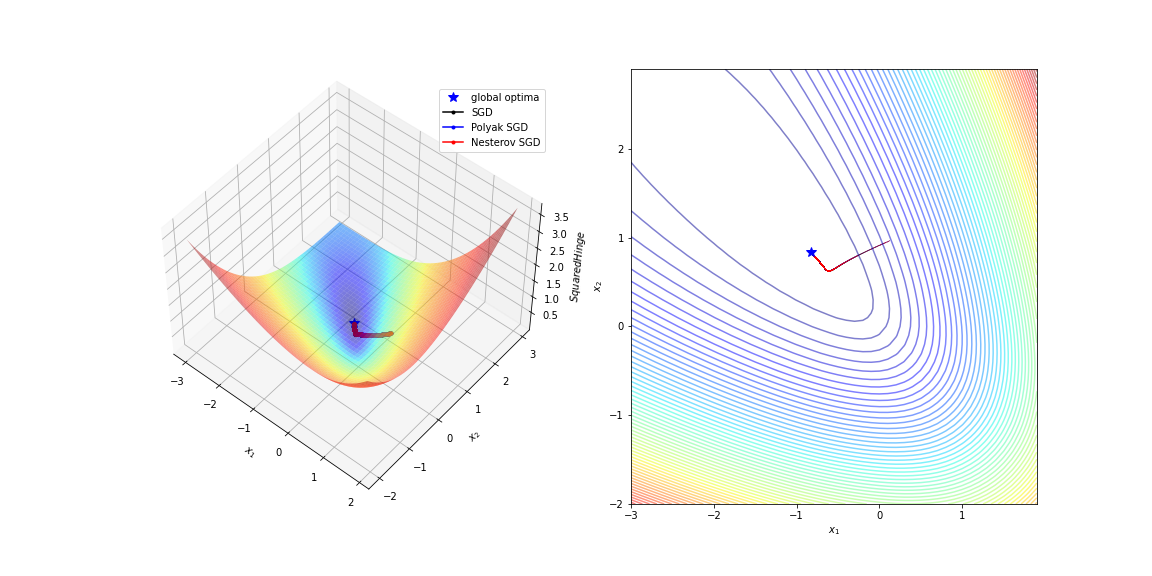
\includegraphics[scale=0.4]{img/l2_svc_loss}
  	\caption{Squared Hinge loss with different optimization steps}
  	\label{fig:l2_svc_loss}
\end{figure}

\subsubsection{Wolfe Dual formulation}

As done for the $\mathcal{L}_1$-SVC we can derive the \emph{Wolfe dual} formulation of the $\mathcal{L}_2$-SVC by obtaining:

\begin{equation} \label{eq:wolfe_dual_l2_svc}
    \begin{aligned}
        \min_{\alpha} \quad & \frac{1}{2}\alpha^T (Q + D)\alpha+q^T\alpha \\
            \text{subject to} \quad & \alpha_i\geq 0 \ \forall_i \\ & y^T\alpha=0
    \end{aligned}
\end{equation}

or, alternatively, with the regularized bias term by obtaining:

\begin{equation} \label{eq:reg_bias_wolfe_dual_l2_svc}
    \begin{aligned}
        \min_{\alpha} \quad & \frac{1}{2}\alpha^T (Q + yy^T + D) \alpha + q^T \alpha \\
            \text{subject to} \quad & \alpha_i \geq 0 \ \forall_i
    \end{aligned}
\end{equation}

where the diagonal matrix $\displaystyle D_{ii} = \frac{1}{2C} \ \forall_i$.

\subsubsection{Lagrangian Dual formulation}

In order to relax the constraints in the $\mathcal{L}_2$-SVC \emph{Wolfe dual} formulation~\eqref{eq:wolfe_dual_l2_svc} we define the problem as a \emph{Lagrangian dual} relaxation by embedding them into objective function, so we need to allocate the Lagrange multipliers $\mu$ and $\lambda \geq 0$:

\begin{equation} \label{eq:l2_svc_lagrangian_dual}
	\begin{aligned}
		    \max_{\mu,\lambda} \min_{\alpha} \mathcal{L}(\alpha,\mu,\lambda) &= \frac{1}{2} \alpha^T (Q+D)\alpha+q^T\alpha - \mu^T (y^T \alpha) - \lambda^T \alpha \\
    &= \frac{1}{2} \alpha^T (Q+D)\alpha + (q - \mu y - \lambda)^T \alpha \\
    \text{subject to} \quad & \,\, \lambda \geq 0
	\end{aligned}
\end{equation}

Taking the derivative of the Lagrangian $\mathcal{L}$ wrt $\alpha$ and settings it to 0 gives:

\begin{equation} \label{eq:l2_svc_lagrangian_der_a}
	\frac{\partial \mathcal{L}}{\partial \alpha}=0\Rightarrow (Q+D) \alpha + (q - \mu y - \lambda) = 0
\end{equation}

With $\alpha$ optimal solution of the linear system:

\begin{equation} \label{eq:l2_svc_lagrangian_sol}
    (Q+D) \alpha = - (q - \mu y - \lambda)
\end{equation}

the gradient wrt $\mu$ and $\lambda$ are:

\begin{equation} \label{eq:l2_svc_lagrangian_der_mu}
	\frac{\partial \mathcal{L}}{\partial \mu}=-y \alpha
\end{equation}

\begin{equation} \label{eq:l2_svc_lagrangian_der_lambda}
    \frac{\partial \mathcal{L}}{\partial \lambda}=-\alpha
\end{equation}

From~\eqref{eq:svc_min_wolfe_dual} we can notice that the equality constraint $y^T \alpha = 0$ arises form the stationarity condition $\partial_{{b}} \mathcal{W}=0$. So, again, for simplicity, we can again consider the bias term $b$ embedded into the weight vector. In this way the dimensionality of~\eqref{eq:l2_svc_lagrangian_dual} is reduced of 1/3 by removing the multipliers $\mu$ which was allocated to control the equality constraint $y^T \alpha=0$, so we will end up solving exactly the problem~\eqref{eq:reg_bias_wolfe_dual_l2_svc}.

\begin{equation} \label{eq:l2_svc_lb_lagrangian_dual}
	\begin{aligned}
    	\max_{\lambda} \min_{\alpha} \mathcal{L}(\alpha,\lambda) &= \frac{1}{2} \alpha^T (Q + yy^T + D) \alpha+q^T\alpha - \lambda^T \alpha \\
    &= \frac{1}{2} \alpha^T (Q + yy^T + D) \alpha + (q - \lambda)^T \alpha \\
    \text{subject to} \quad & \,\, \lambda \geq 0
	\end{aligned}
\end{equation}

where, again, the upper bound $u^T = [C, \dots, C]$.

Now, taking the derivative of the Lagrangian $\mathcal{L}$ wrt $\alpha$ and settings it to 0 gives:

\begin{equation} \label{eq:l2_svc_lb_lagrangian_der_a}
	\frac{\partial \mathcal{L}}{\partial \alpha}=0\Rightarrow (Q + yy^T + D) \alpha + (q - \lambda) = 0
\end{equation}

With $\alpha$ optimal solution of the linear system:

\begin{equation} \label{eq:l2_svc_lb_lagrangian_sol}
    (Q + yy^T + D) \alpha = - (q - \lambda)
\end{equation}

the gradient wrt $\lambda$ is:

\begin{equation} \label{eq:l2_svc_lb_lagrangian_der_l}
    \frac{\partial \mathcal{L}}{\partial \lambda}=-\alpha
\end{equation}

\pagebreak

\section{Linear Support Vector Regression}

In the case of regression the goal is to predict a real-valued output for $y'$ so that our training data is of the form:

\begin{equation}
	\{(x_i,y_i), x\in\Re^m, y_i\in\Re, i=1, \dots, n\} \label{eq:svr_data}
\end{equation}

The regression SVM use a loss function that not allocating a penalty if the predicted value $y'_i$ is less than a distance $\epsilon$ away from the actual value $y_i$, i.e., if $|y_i-y'_i| \leq \epsilon$, where $y'_i = w^T x_i + b$. The region bound by $y'_i\pm\epsilon \ \forall_i$ is called an $\epsilon$-insensitive tube. The output variables which are outside the tube are given one of two slack variable penalties depending on whether they lie above, $\xi^+$, or below, $\xi^-$, the tube, provided $\xi^+ \geq 0$ and $\xi^- \geq 0 \ \forall_i$:

\begin{equation} \label{eq:svr_consts}
	\begin{aligned}
		& y_i\leq y'_i+\epsilon+\xi^+ \ \forall_i \\
    	& y_i\geq y'_i-\epsilon-\xi^- \ \forall_i \\
    	& \xi_i^+, \xi_i^- \geq 0 \ \forall_i
	\end{aligned}
\end{equation}

The objective function for SVR can then be written as:

\begin{equation} \label{eq:quad_svr_obj}
    \begin{aligned}
        \min_{w,b,\xi^+,\xi^-} \quad & \frac{1}{2} \| w \|^2 + C \sum_{i=1}^n (\xi_i^+ + \xi_i^-) \\
            \text{subject to} \quad & y_i - w^T x_i - b \leq \epsilon + \xi_i^+ \ \forall_i \\ & w^T x_i + b - y_i \leq \epsilon + \xi_i^- \ \forall_i \\ & \xi_i^+, \xi_i^- \geq 0 \ \forall_i
    \end{aligned}
\end{equation}

\begin{figure}[h!]
	\centering
  	\includegraphics[scale=0.6]{img/linear_dual_svr_hyperplane}
  	\caption{Linear SVR hyperplane}
  	\label{fig:linear_dual_svr_hyperplane}
\end{figure}

\subsection{Epsilon-insensitive loss}

The \emph{epsilon-insensitive} loss is defined as:

\begin{equation} \label{eq:eps_loss1}
	\mathcal{L}_\epsilon^1 = 
	\begin{cases}
		0 & \text{if} \ |y - (w^T x + b)| \leq \epsilon \\
		|y - (w^T x + b)| - \epsilon & \text{otherwise} \\
	\end{cases}
\end{equation}

or, equivalently:

\begin{equation} \label{eq:eps_loss2}
	\mathcal{L}_\epsilon^1 = \max(0, |y - (w^T x + b)| - \epsilon)
\end{equation}

As the \emph{hinge} loss, also the \emph{epsilon-insensitive} loss is a nondifferentiable convex function due to its nonsmoothness in $\pm\epsilon$, but has a subgradient wrt $w$ that is given by:

\begin{equation} \label{eq:eps_loss_der}
	\frac{\partial \mathcal{L_\epsilon^1}}{\partial w}=
		\begin{cases}
            (y - (w^T x + b)) x & \text{if} \ |y - (w^T x + b)| > \epsilon \\
            0 & \text{otherwise} \\ 
        \end{cases}
\end{equation}

\subsubsection{Primal formulation}

The general primal unconstrained formulation takes the same form of~\eqref{eq:primal_svc}.

The quadratic optimization problem~\eqref{eq:quad_svr_obj} can be equivalently formulated as:

\begin{equation} \label{eq:svr_eps}
	\min_{w,b} \frac{1}{2} \| w \|^2 + C \sum_{i=1}^n \max(0, |y_i - (w^T x_i + b)| - \epsilon)
\end{equation}

where we make use of the \emph{epsilon-insensitive} loss~\eqref{eq:eps_loss1} or~\eqref{eq:eps_loss2}.

The above formulation penalizes slacks $\xi$ linearly and is called $\mathcal{L}_1$-SVR.

\begin{figure}[h!]
	\centering
  	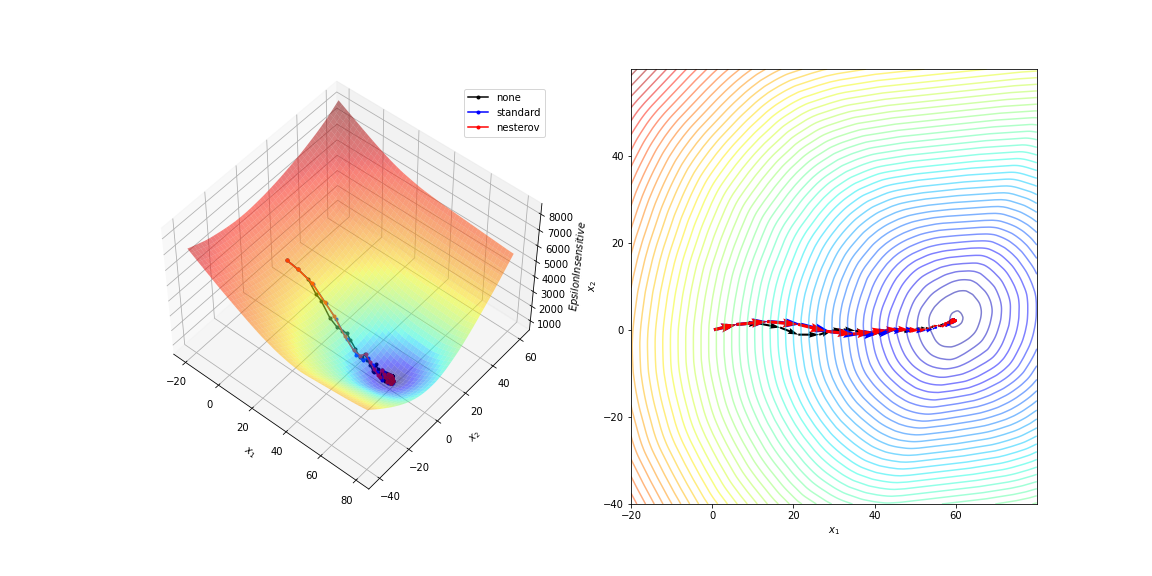
\includegraphics[scale=0.4]{img/svr_eps_loss}
  	\caption{SVR Epsilon-insensitive loss with different optimization steps}
  	\label{fig:svr_eps_loss}
\end{figure}

\subsubsection{Wolfe Dual formulation}

To reformulate the~\eqref{eq:quad_svr_obj} as a \emph{Wolfe dual}, we introduce the Lagrange multipliers $\alpha_i^+ \geq 0, \alpha_i^- \geq 0, \mu_i^+ \geq 0, \mu_i^- \geq 0 \ \forall_i$:

\begin{equation} \label{eq:svr_wolfe_dual}
	\begin{aligned}
    	\max_{\alpha^+,\alpha^-,\mu^+,\mu^-} \min_{w,b,\xi^+,\xi^-} \mathcal{W}(w,b,\xi^+,\xi^-,\alpha^+,\alpha^-,\mu^+,\mu^-) = \frac{1}{2} \| w \|^2 + C \sum_{i=1}^n (\xi_i^+ + \xi_i^-)-\sum_{i=1}^n (\mu_i^+ \xi_i^+ + \mu_i^- \xi_i^-) \\ -\sum_{i=1}^n \alpha_i^+(\epsilon+\xi_i^+ + y'_i-y_i)-\sum_{i=1}^n \alpha_i^-(\epsilon+\xi_i^- - y'_i+y_i)
	\end{aligned}
\end{equation}

Substituting for $y_i$, differentiating wrt $w, b, \xi^+$, $\xi^-$ and setting the derivatives to $0$ gives:

\begin{equation} \label{eq:svr_wolfe_der_w}
	\frac{\partial \mathcal{W}}{\partial w}=w-\sum_{i=1}^n (\alpha_i^+ - \alpha_i^-) x_i \Rightarrow w=\sum_{i=1}^n (\alpha_i^+ - \alpha_i^-) x_i
\end{equation}

\begin{equation} \label{eq:svr_wolfe_der_b}
	\frac{\partial \mathcal{W}}{\partial b}=-\sum_{i=1}^n (\alpha_i^+ - \alpha_i^-)\Rightarrow \sum_{i=1}^n (\alpha_i^+ - \alpha_i^-)=0
\end{equation}

\begin{equation}\label{eq:svr_wolfe_der_xip}
	\frac{\partial \mathcal{W}}{\partial\xi_i^+}=0\Rightarrow C=\alpha_i^+ + \mu_i^+
\end{equation}

\begin{equation} \label{eq:svr_wolfe_der_xim}
	\frac{\partial \mathcal{W}}{\partial\xi_i^-}=0\Rightarrow C=\alpha_i^- + \mu_i^-
\end{equation}

Substituting~\eqref{eq:svr_wolfe_der_w} and~\eqref{eq:svr_wolfe_der_b} in, we now need to maximize $\mathcal{W}$ wrt $\alpha_i^+$ and $\alpha_i^-$, where $\alpha_i^+ \geq 0,\ \alpha_i^- \geq 0 \ \forall_i$:

\begin{equation} \label{eq:svr_max_wolfe_dual}
    \max_{\alpha^+,\alpha^-} \mathcal{W}(\alpha^+,\alpha^-) = \sum_{i=1}^n y_i(\alpha_i^+ - \alpha_i^-)-\epsilon\sum_{i=1}^n (\alpha_i^+ + \alpha_i^-)-\frac{1}{2}\sum_{i,j}(\alpha_i^+ - \alpha_i^-)\langle x_i, x_j \rangle(\alpha_j ^+ - \alpha_j ^-)
\end{equation}

Using $\mu_i^+ \geq 0$ and $\mu_i^- \geq 0$ together with~\eqref{eq:svr_wolfe_der_w} and~\eqref{eq:svr_wolfe_der_b} means that $\alpha_i^+ \leq C$ and $\alpha_i^- \leq C$. We therefore need to find:

\begin{equation} \label{eq:svr_min_wolfe_dual}
    \begin{aligned}
        \min_{\alpha^+,\alpha^-} \quad & \frac{1}{2}(\alpha^+ - \alpha^-)^TK(\alpha^+ - \alpha^-)+\epsilon q^T(\alpha^+ + \alpha^-)-y^T(\alpha^+ - \alpha^-) \\
            \text{subject to} \quad & 0\leq\alpha_i^+,\alpha_i^- \leq C \ \forall_i \\ & q^T(\alpha^+ - \alpha^-)=0
    \end{aligned}
\end{equation}

where $q^T = [1, \dots, 1]$.

We can write the~\eqref{eq:svr_min_wolfe_dual} in a standard quadratic form as:

\begin{equation}
    \begin{aligned} \label{eq:svr_min_qp_wolfe_dual}
        \min_{\alpha} \quad & \frac{1}{2}\alpha^T Q\alpha-q^T\alpha \\
            \text{subject to} \quad & 0\leq\alpha_i\leq C \ \forall_i \\ & e^T\alpha=0
    \end{aligned}
\end{equation}

where the Hessian matrix $Q$ is 
$
\begin{bmatrix}
K & -K\\
-K & K 
\end{bmatrix}$
, $q$ is 
$
\begin{bmatrix}
-y\\
y
\end{bmatrix}$ + $\epsilon$
, and $e$ is 
$
\begin{bmatrix}
1\\
-1
\end{bmatrix}$.

Each new predictions $y'$ can be found using:

\begin{equation} \label{eq:svr_pred}
    y'= \sum_{i=1}^n (\alpha_i^+ - \alpha_i^-)\langle x_i, x' \rangle+b
\end{equation}

A set $S$ of support vectors $x_s$ can be created by finding the indices $i$ where $0\leq\alpha\leq C$ and $\xi_i^+=0$ or $\xi_i^-=0$.

This gives us:

\begin{equation} \label{eq:svr_b}
    b=y_s-\epsilon-\sum_{m\in S}(\alpha_m^+ -\alpha_m^-) \langle x_m, x_s \rangle
\end{equation}

As before it is better to average over all the indices $i$ in $S$:

\begin{equation} \label{eq:svr_b_avg}
    b=\frac{1}{N_s}\sum_{s\in S}y_s-\epsilon-\sum_{m \in S}(\alpha_m^+ - \alpha_m^-)\langle x_m, x_s \rangle
\end{equation}

From~\eqref{eq:svr_min_qp_wolfe_dual} we can notice that the equality constraint $e^T \alpha = 0$ arises form the stationarity condition $\partial_{{b}} \mathcal{W}=0$. So, again, for simplicity, we can again consider the bias term $b$ embedded into the weight vector. We report below the box-constrained dual formulation~\cite{hsu2002simple} that arises from the primal~\eqref{eq:primal_svc_hinge1} or~\eqref{eq:primal_svc_hinge2} where the bias term $b$ is embedded into the weight vector $w$:

\begin{equation} \label{eq:svr_min_bcqp_wolf_dual}
    \begin{aligned}
        \min_{\alpha} \quad & \frac{1}{2} \alpha^T (Q + ee^T)\alpha+q^T\alpha \\
            \text{subject to} \quad & 0\leq\alpha_i\leq C \ \forall_i
    \end{aligned}
\end{equation}

\subsubsection{Lagrangian Dual formulation}

In order to relax the constraints in the \emph{Wolfe dual} formulation~\eqref{eq:svr_min_wolfe_dual} we define the problem as a \emph{Lagrangian dual} relaxation by embedding them into objective function, so we need to allocate the Lagrangian multipliers $\mu \geq 0, \lambda_+ \geq 0$, $\lambda_- \geq 0$:

\begin{equation} \label{eq:svr_lagrangian_dual}
	\begin{aligned}
		    \max_{\mu,\lambda_+,\lambda_-} \min_{\alpha} \mathcal{L}(\alpha,\mu,\lambda_+,\lambda_-) &= \frac{1}{2} \alpha^T Q\alpha+q^T\alpha - \mu^T (e^T \alpha) - \lambda_+^T (u - \alpha) - \lambda_-^T \alpha \\
    &= \frac{1}{2} \alpha^T Q\alpha + (q - \mu e + \lambda_+ - \lambda_-)^T \alpha - \lambda_+^T u
	\end{aligned}
\end{equation}

where the upper bound $u^T = [C, \dots, C]$.

Taking the derivative of the Lagrangian $\mathcal{L}$ wrt $\alpha$ and settings it to 0 gives:

\begin{equation} \label{eq:svr_lagrangian_der_a}
	\frac{\partial \mathcal{L}}{\partial \alpha}=0\Rightarrow Q \alpha + (q - \mu e + \lambda_+ - \lambda_-) = 0
\end{equation}

With $\alpha$ optimal solution of the linear system:

\begin{equation} \label{eq:svr_lagrangian_sol}
    Q \alpha = - (q - \mu e + \lambda_+ - \lambda_-)
\end{equation}

the gradient wrt $\mu$, $\lambda_+$ and $\lambda_-$ are:

\begin{equation} \label{eq:svr_lagrangian_der_mu}
	\frac{\partial \mathcal{L}}{\partial \mu}=-e \alpha
\end{equation}

\begin{equation} \label{eq:svr_lagrangian_der_lp}
	\frac{\partial \mathcal{L}}{\partial \lambda_+}=\alpha - u
\end{equation}

\begin{equation} \label{eq:svr_lagrangian_der_lm}
    \frac{\partial \mathcal{L}}{\partial \lambda_-}=-\alpha
\end{equation}

If the Hessian matrix Q is not positive definite, i.e., the Lagrangian function is not strictly convex since it will be linear along the eigenvectors correspondent to the null eigenvalues and so it will be unbounded below, the Lagrangian dual relaxation will be nondifferentiable, so it will have infinite solutions and for each of them it will have a different subgradient. In order to compute an approximation of the gradient, we will choose $\alpha$ in such a way as the one that minimizes the norm of the residual:

\begin{equation} \label{eq:svr_lagrangian_krylov_sol}
	\begin{aligned}
		\min_{\alpha_n \in K_n(Q, b)} \quad & \| Q \alpha_n - b \| \\ 
		\text{where} \quad & b = - (q - \mu e + \lambda_+ - \lambda_-)
	\end{aligned}
\end{equation}

Since we are dealing with a symmetric but indefinite linear system we will choose a well-known Krylov method that performs the Lanczos iterate, i.e., symmetric Arnoldi iterate, called \emph{minres}, i.e., symmetric \emph{gmres}, to compute the vector $\alpha_n$ that minimizes the norm of the residual $r_n = Q \alpha_n - b$ among all vectors in $K_n(Q, b) = span(b, Qb, Q^2b, \dots, Q^{n-1}b)$.

\bigskip

From~\eqref{eq:svr_min_qp_wolfe_dual} we can notice that the equality constraint $e^T \alpha = 0$ arises form the stationarity condition $\partial_{{b}} \mathcal{W}=0$. So, again, for simplicity, we can again consider the bias term $b$ embedded into the weight vector. In this way the dimensionality of~\eqref{eq:svr_lagrangian_dual} is reduced of 1/3 by removing the multipliers $\mu$ which was allocated to control the equality constraint $e^T \alpha=0$, so we will end up solving exactly the problem~\eqref{eq:svr_min_bcqp_wolf_dual}.

\begin{equation} \label{eq:svr_bcqp_lagrangian_dual}
	\begin{aligned}
    	\max_{\lambda_+,\lambda_-} \min_{\alpha} \mathcal{L}(\alpha,\lambda_+,\lambda_-) &= \frac{1}{2} \alpha^T (Q + ee^T)\alpha+q^T\alpha - \lambda_+^T (u - \alpha) - \lambda_-^T \alpha \\
    &= \frac{1}{2} \alpha^T (Q + ee^T)\alpha + (q + \lambda_+ - \lambda_-)^T \alpha - \lambda_+^T u
	\end{aligned}
\end{equation}

where, again, the upper bound $u^T = [C, \dots, C]$.

Now, taking the derivative of the Lagrangian $\mathcal{L}$ wrt $\alpha$ and settings it to 0 gives:

\begin{equation} \label{eq:svr_bcqp_lagrangian_der_a}
	\frac{\partial \mathcal{L}}{\partial \alpha}=0\Rightarrow (Q + ee^T) \alpha + (q + \lambda_+ - \lambda_-) = 0
\end{equation}

With $\alpha$ optimal solution of the linear system:

\begin{equation} \label{eq:svr_bcqp_lagrangian_sol}
    (Q + ee^T) \alpha = - (q + \lambda_+ - \lambda_-)
\end{equation}

the gradient wrt $\lambda_+$ and $\lambda_-$ are:

\begin{equation} \label{eq:svr_bcqp_lagrangian_der_lp}
	\frac{\partial \mathcal{L}}{\partial \lambda_+}=\alpha - u
\end{equation}

\begin{equation} \label{eq:svr_bcqp_lagrangian_der_lm}
    \frac{\partial \mathcal{L}}{\partial \lambda_-}=-\alpha
\end{equation}

\subsection{Squared Epsilon-insensitive loss}

The \emph{squared epsilon-insensitive} loss is defined as:

\begin{equation} \label{eq:squared_eps_loss1}
	\mathcal{L}_\epsilon^2 = 
	\begin{cases}
		0 & \text{if} \ |y - (w^T x + b)| \leq \epsilon \\
		(|y - (w^T x + b)| - \epsilon)^2 & \text{otherwise} \\
	\end{cases}
\end{equation}

or, equivalently:

\begin{equation} \label{eq:squared_eps_loss2}
	\mathcal{L}_\epsilon^2 = \max(0, |y - (w^T x + b)| - \epsilon)^2
\end{equation}

As the \emph{squared hinge} loss, also the \emph{squared epsilon-insensitive} loss is a strictly convex function and it has a gradient wrt $w$ that is given by:

\begin{equation} \label{eq:squared_eps_loss_der}
	\frac{\partial \mathcal{L}_\epsilon^2}{\partial w}=
		\begin{cases}
            2 ((y - (w^T x + b)) x) & \text{if} \ |y - (w^T x + b)| > \epsilon \\
            0 & \text{otherwise} \\ 
        \end{cases}
\end{equation}

\subsubsection{Primal formulation}

To provide a continuously differentiable function the optimization problem~\eqref{eq:svr_eps} can be formulated as:

\begin{equation} \label{eq:svr_squared_eps}
    \min_{w,b} \frac{1}{2} \| w \|^2 + C \sum_{i=1}^n \max(0, |y_i - (w^T x_i + b)| - \epsilon)^2
\end{equation}

where we make use of the \emph{squared epsilon-insensitive} loss that quadratically penalized slacks $\xi$ and is called $\mathcal{L}_2$-SVR.

\begin{figure}[h!]
	\centering
  	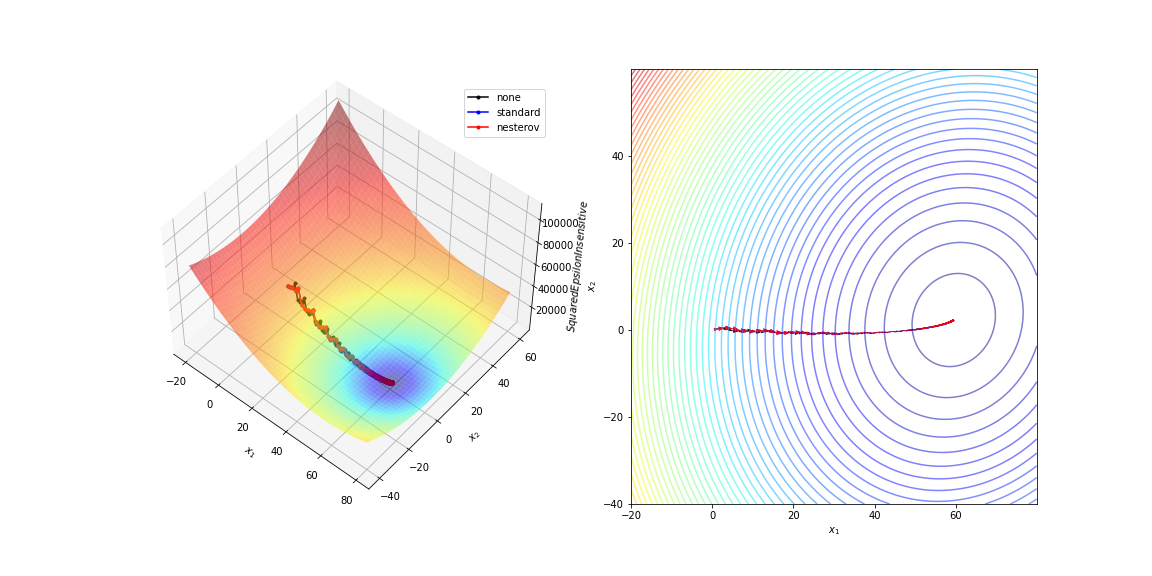
\includegraphics[scale=0.4]{img/svr_squared_eps_loss}
  	\caption{SVC Squared Epsilon-insensitive loss with different optimization steps}
  	\label{fig:svr_squared_eps_loss}
\end{figure}


\pagebreak

\section{Nonlinear Support Vector Machines}

When applying our SVC to \emph{linearly separable} data in~\eqref{eq:svc_max_wolfe_dual}, we have started by creating a matrix $Q$ from the dot product of our input variables:

\begin{equation} \label{eq:svc_hessian}
	Q_{ij} = y_i y_j k(x_i,x_j)
\end{equation}

or, a matrix $K$ from the dot product of our input variables in the SVR case~\eqref{eq:svr_min_wolfe_dual}:

\begin{equation} \label{eq:svr_hessian}
	K_{ij} = k(x_i,x_j)
\end{equation}

where $k(x_i,x_j)$ is an example of a family of functions called \emph{kernel functions}.

For any positive definite kernel function $k$ (a so called Mercer kernel), it is guaranteed that there exists a mapping $\phi$ into a Hilbert space $\mathcal{H}$, such that:

\begin{equation} \label{eq:kernel_function}
	k(x_i,x_j) = \langle \phi(x_i), \phi(x_j) \rangle = \phi(x_i)^T \phi(x_j)
\end{equation}

where $\langle \cdot, \cdot \rangle$ denotes the inner product in the Hilbert space and $\phi(\cdot)$ is the identity function.

The reason that this \emph{kernel trick} is useful is that there are many classification/regression problems that are nonlinearly separable/regressable in the \emph{input space}, which might be in a higher dimensionality \emph{feature space} given a suitable mapping $x \rightarrow \phi(x)$.

\subsection{Polynomial kernel}

The \emph{polynomial} kernel is defined as:

\begin{equation} \label{eq:poly_kernel}
	k(x_i,x_j)=(\gamma \langle x_i, x_j\rangle + r)^d
\end{equation}

where $\gamma$ define how far the influence of a single training example reaches (low values meaning ‘far’ and high values meaning ‘close’).

\begin{figure}[h!]
	\centering
	\begin{subfigure}{.49\textwidth}
		\centering
		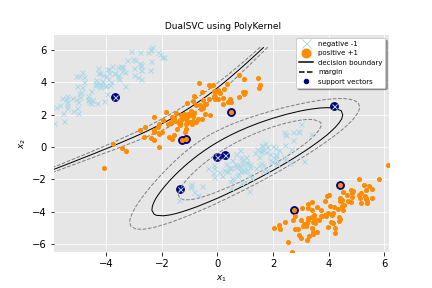
\includegraphics[width=\textwidth]{img/poly_dual_l1_svc_hyperplane}
		\caption{Polynomial SVC hyperplane}
		\label{fig:poly_dual_l1_svc_hyperplane}
	\end{subfigure}
	\begin{subfigure}{.49\textwidth}
		\centering
		\captionsetup{justification=centering}
		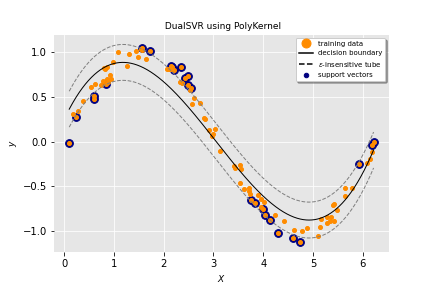
\includegraphics[width=\textwidth]{img/poly_dual_l1_svr_hyperplane}
		\caption{Polynomial SVR hyperplane}
		\label{fig:poly_dual_l1_svr_hyperplane}
	\end{subfigure}
\caption{Polynomial SVM hyperplanes}
\end{figure}

\subsection{Gaussian RBF kernel}

The \emph{gaussian} kernel is defined as:

\begin{equation} \label{eq:gaussian_kernel1}
	k(x_i,x_j)=\exp(-\frac{\|x_i-x_j\|^2}{2\sigma^2})
\end{equation}

or, equivalently:

\begin{equation} \label{eq:gaussian_kernel2}
	k(x_i,x_j)=\exp(-\gamma \|x_i-x_j\|^2)
\end{equation}

where $\displaystyle \gamma=\frac{1}{2\sigma^2}$ define how far the influence of a single training example reaches (low values meaning ‘far’ and high values meaning ‘close’).

\begin{figure}[h!]
	\centering
	\begin{subfigure}{.49\textwidth}
		\centering
		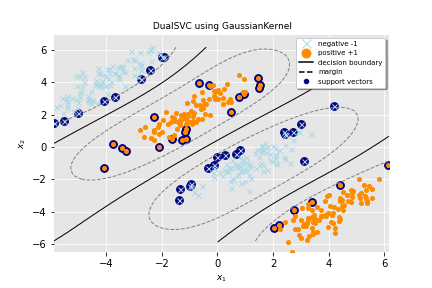
\includegraphics[width=\textwidth]{img/gaussian_dual_l1_svc_hyperplane}
		\caption{Gaussian SVC hyperplane}
		\label{fig:gaussian_dual_l1_svc_hyperplane}
	\end{subfigure}
	\begin{subfigure}{.49\textwidth}
		\centering
		\captionsetup{justification=centering}
		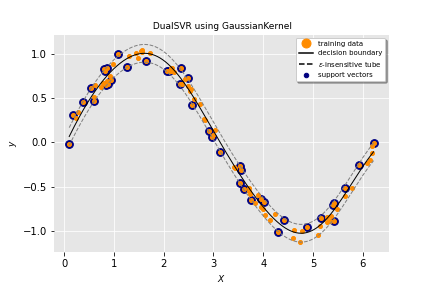
\includegraphics[width=\textwidth]{img/gaussian_dual_l1_svr_hyperplane}
		\caption{Gaussian SVR hyperplane}
		\label{fig:gaussian_dual_l1_svr_hyperplane}
	\end{subfigure}
\caption{Gaussian SVM hyperplanes}
\end{figure}

\pagebreak

\section{Optimization Methods}

In order to explain the \emph{convergence} and \emph{efficiency} properties of the following optimization methods, we need to introduce some preliminary definitions about \emph{convexity} and the \emph{L-smoothness} of a function~\cite{boyd2004convex}.

\begin{definition}[Convexity] \label{def:convexity}
	\hfill
	\begin{enumerate}[i]
		\item We say that a function $f: \Re^m \rightarrow \Re$ is convex if: 
		$$ 
			(\lambda x + (1 - \lambda) y ) \leq \lambda f(x) + (1 - \lambda) f(y) \ \forall \ x, y \in \Re^m, \lambda \in [0,1] 
		$$
		\item We say that a differentiable function $f: \Re^m \rightarrow \Re$, i.e., $f \in C^1$, is convex if: 
		$$ 
			f(y) \geq f(x) + \langle \nabla f(x), y - x \rangle \ \forall \ x, y \in \Re^m 
		$$
		\item We say that a twice differentiable function $f: \Re^m \rightarrow \Re$, i.e., $f \in C^2$ and the Hessian matrix is symmetric, is convex iff: 
		$$ 
			\nabla^2 f(x) \succeq 0 \ \forall \ x \in \Re^m 
		$$ i.e., the Hessian matix is \emph{positive semidefinite}.
	\end{enumerate}
\end{definition}

\begin{definition}[Strict Convexity] \label{def:strict_convexity}
	\hfill
	\begin{enumerate}[i]
		\item We say that a function $f: \Re^m \rightarrow \Re$ is strictly convex if: 
		$$ 
			(\lambda x + (1 - \lambda) y ) < \lambda f(x) + (1 - \lambda) f(y) \ \forall \ x, y \in \Re^m, x \neq y, \lambda \in (0,1) 
		$$
		\item We say that a differentiable function $f: \Re^m \rightarrow \Re$, i.e., $f \in C^1$, is strictly convex if: 
		$$ 
			f(y) > f(x) + \langle \nabla f(x), y - x \rangle \ \forall \ x, y \in \Re^m, x \neq y
		$$
		\item We say that a twice differentiable function $f: \Re^m \rightarrow \Re$, i.e., $f \in C^2$ and the Hessian matrix is symmetric, is strictly convex iff: 
		$$ 
			\nabla^2 f(x) \succ 0 \ \forall \ x \in \Re^m 
		$$ i.e., the Hessian matix is \emph{positive definite}.
	\end{enumerate}
\end{definition}

\begin{definition}[Strong Convexity] \label{def:strong_convexity}
We say that a function $f: \Re^m \rightarrow \Re$ is $\mu$-strongly convex if the function:
$$
g(x) = f(x) - \frac{\mu}{2} \| x \|^2
$$
is convex for any $\mu > 0$. 
If $f$ is differentiable, i.e., $f \in C^1$, this is also equivalent to:
$$
f(y) \geq f(x) + \langle \nabla f(x), y - x \rangle + \frac{\mu}{2} \| y - x \|^2 \ \forall \ x, y \in \Re^m
$$
and, if $f$ is a twice differentiable function, i.e., $f \in C^2$ and the Hessian matrix is symmetric, then $f$ is $\mu$-strongly convex iff:
$$
\nabla^2 g(x) \succ 0 \ \forall \ x \in \Re^m
$$
i.e., the Hessian matix is \emph{positive definite}, which is:
$$
\nabla^2 f(x) \succeq \mu I \ \forall \ x \in \Re^m
$$
\end{definition}

\begin{definition}[L-smoothness] \label{def:l_smoothness}
We say that a function $f: \Re^m \rightarrow \Re$ is L-smooth, i.e., L-Lipschitz continuous, if it is differentiable, i.e., $f \in C^1$, and if:
$$
\| \nabla f(x) - \nabla f(y) \| \leq L \| x - y \| \ \forall \ x, y \in \Re^m
$$
then:
$$
f(y) \leq f(x) + \langle \nabla f(x), y - x \rangle + \frac{L}{2} \| y - x \|^2 \ \forall \ x, y \in \Re^m
$$
and, if $f$ is a $\mu$-strongly convex function, we give the following Hessian bounds:
$$
0 \prec \mu I \preceq \nabla^2 f(x) \preceq L I \ \forall \ x \in \Re^m
$$
\end{definition}

\pagebreak

\subsection{Gradient Descent for Primal formulations}

The Gradient Descent algorithm is the simplest \emph{first-order optimization} method that exploits the orthogonality of the gradient wrt the level sets to take a descent direction. In particular, it performs the following iterations:

\begin{algorithm}[H]
	\caption{Gradient Descent}
	\label{alg:gd}
	\begin{algorithmic}
		\Require{Function $f$ to minimize}
		\Require{Learning rate or step size $\alpha > 0$}
		\Function{GradientDescent}{$f,\alpha$}
			\State Initialize weight vector $x_0$
			\State $t = 0$
			\While{$not\_convergence$}
				\State $x_{t+1} = x_t - \alpha \nabla f(x_t)$
				\State $t = t + 1$
			\EndWhile
			\State \Return $x_t$
		\EndFunction
	\end{algorithmic}
\end{algorithm}

\begin{theorem}[Gradient Descent convergence for convex functions] \label{thm:cvx_gd_convergence}
Let $f: \Re^m \rightarrow \Re$ be a L-smooth convex function. Then the Gradient Descent with step size $\alpha \leq 1/L$ satisfies:
$$
f(x_t) - f(x^*) \leq \frac{\| x_0 - x^* \|^2}{2 \alpha t}
$$
In particular, for $\alpha = 1/L$:
$$
f(x_t) - f(x^*) \leq \frac{L \| x_0 - x^* \|^2}{2 t}
$$
\end{theorem}

\begin{theorem}[Gradient Descent convergence for strongly convex functions] \label{thm:str_cvx_gd_convergence}
Let $f: \Re^m \rightarrow \Re$ be a L-smooth and $\mu$-strongly convex function. Then the Gradient Descent with step size $\alpha \leq 1/L$ satisfies:
$$
f(x_t) - f(x^*) \leq (1 - \alpha \mu)^t \| x_0 - x^* \|^2
$$
In particular, for $\alpha = 1/L$:
$$
\begin{aligned}
	f(x_t) - f(x^*) \leq & \bigg(1 - \frac{\mu}{L}\bigg)^t \| x_0 - x^* \|^2 \\
						= & \bigg(1 - \frac{1}{\kappa}\bigg)^t \| x_0 - x^* \|^2
\end{aligned}
$$
where $\kappa = L/\mu$.
\end{theorem}

\begin{theorem}[Gradient Descent convergence for quadratic functions] \label{thm:quad_gd_convergence}
Let $f: \Re^m \rightarrow \Re$ be a L-smooth and $\mu$-strongly convex quadratic function. Then the Gradient Descent with step size $\alpha = \displaystyle \frac{2}{L + \mu}$ and momentum $\beta = \displaystyle \frac{\kappa-1}{\kappa+1} = 1 - \frac{2}{\kappa+1}$ satisfies:
$$
\begin{aligned}
	\| x_t - x^* \| = \bigg(\frac{\kappa-1}{\kappa+1}\bigg)^t \| x_0 - x^* \|
\end{aligned}
$$
where $\kappa = L/\mu$.
\end{theorem}

Gradient Descent is based on full gradients, since at each iteration we compute the average gradient on the whole dataset:
$$
\nabla f(x) = \frac{1}{n} \sum_{i=1}^n \nabla f_i(x)
$$
The downside is that every step is very computationally expensive, $\mathcal{O}(nm)$ per iteration, where $n$ is the number of samples in our dataset and $m$ is the number of dimensions.

Since \emph{Gradient Descent} becomes impractical when dealing with large datasets we introduce a stochastic version, called \emph{Stochastic Gradient Descent}, which does not use the whole set of examples to compute the gradient at every step. By doing so, we can reduce computation all the way down to $\mathcal{O}(m)$ per iteration.

\begin{algorithm}[H]
	\caption{Stochastic Gradient Descent}
	\label{alg:sgd}
	\begin{algorithmic}
		\Require{Function $f$ to minimize}
		\Require{Learning rate or step size $\alpha > 0$}
		\Require{Batch size $k$}
		\Function{StochasticGradientDescent}{$f,\alpha,k$}
			\State Initialize weight vector $x_0$
			\State $t \gets 0$
			\While{$not\_convergence$}
				\State Sample $(i_1,\dots,i_k) \sim \mathcal{U}^k(1,\dots,n)$ 
				\State $\displaystyle x_{t+1} \gets x_t - \alpha \frac{1}{k} \sum_{j=1}^k \nabla f_{i_j}(x_t)$
				\State $t \gets t + 1$
			\EndWhile
			\State \Return $x_t$
		\EndFunction
	\end{algorithmic}
\end{algorithm}

Note that in expectation, we converge like GD, since $\displaystyle \mathbb{E}_{i \sim \mathcal{U}(1,\dots,n)}[\nabla f_i(x_t)] = \nabla f(x_t)$, therefore, the expected iterate of SGD converges to the optimum.

Consider the SGD algorithm introduced previously but where each iteration is projected into the ball $\mathcal{B}(0, R)$ with radius $R > 0$ fixed.

\begin{theorem}[Stochastic Gradient Descent convergence for convex functions] \label{thm:cvx_sgd_convergence}
Let $f: \Re^m \rightarrow \Re$ be a L-smooth convex function and assume that exists $b > 0$ satisfying:
$$
\| f_i(x) \| \leq b \ \forall \ x \in \mathcal{B}(0, R)
$$
Besides, assume that all minima of $f$ belong to $\mathcal{B}(0, R)$. Then the Stochastic Gradient Descent with step size $\alpha = 2R/(b\sqrt{k})$ satisfies:
$$
\mathbb{E}\Bigg[f\Bigg(\frac{1}{k} \sum_{t=1}^k x_t\Bigg)\Bigg] - f(x^*) \leq \frac{3Rb}{\sqrt{k}}
$$
\end{theorem}

\begin{theorem}[Stochastic Gradient Descent convergence for strongly convex functions] \label{thm:str_cvx_sgd_convergence}
Let $f: \Re^m \rightarrow \Re$ be a L-smooth, $\mu$-strongly convex function and assume that exists $b > 0$ satisfying:
$$
\| f_i(x) \| \leq b \ \forall \ x \in \mathcal{B}(0, R)
$$
Besides, assume that all minima of $f$ belong to $\mathcal{B}(0, R)$. Then the Stochastic Gradient Descent with step size $\alpha = 2/(\mu(k+1))$ satisfies:
$$
\mathbb{E}\Bigg[f\Bigg(\frac{2}{k(k+1)} \sum_{t=1}^k t x_{t-1}\Bigg)\Bigg] - f(x^*) \leq \frac{2b^2}{\mu(k+1)}
$$
\end{theorem}

SGD’s \emph{convergence rate} for L-smooth convex functions is $\displaystyle \mathcal{O}\bigg(\frac{1}{\sqrt{t}}\bigg)$ and $\displaystyle \mathcal{O}\bigg(\frac{1}{t}\bigg)$ for strongly convex. More iterations are needed to reach the same accuracy as GD, but the iterations are far cheaper.

\subsubsection{Momentum}

To mitigate the pathological zig-zagging by speeding up the \emph{convergence rate} of the SGD method, we introduce two accelerated methods~\cite{polyak1964some} and~\cite{nesterov1998introductory, nesterov1983method} that exploits information from the history, i.e., past iterates, to add some inertia, i.e., the momentum, to yield smoother trajectory.

In the Polyak's method~\cite{polyak1964some} the velocity vector $v_t$ is calculated by applying the $\beta$ momentum to the previous $v_{t-1}$ displacement, and subtracting the gradient step to $x_t$.

\begin{figure}[h!]
	\centering
  	\includegraphics[scale=0.5]{img/momentum}
  	\caption{Polyak's and Nesterov's Momentum}
  	\label{fig:momentum}
\end{figure}

\begin{algorithm}[H]
	\caption{Polyak's Accelerated Gradient Descent or Polyak Heavy-Ball method}
	\label{alg:pag}
	\begin{algorithmic}
		\Require{Function $f$ to minimize}
		\Require{Learning rate or step size $\alpha > 0$}
		\Require{Momentum $\beta \in [0,1)$}
		\Function{PolyakAcceleratedGradientDescent}{$f,\alpha,\beta$}
			\State Initialize weight vector $x_1 \gets x_0$ and velocity vector $v_0 \gets 0$
			\State $t \gets 1$
			\While{$not\_convergence$}
				\State $v_t = \beta v_{t-1} + \alpha \nabla f(x_t)$
				\State $x_{t+1} = x_t - v_t$
				\State $t \gets t + 1$
			\EndWhile
			\State \Return $x_t$
		\EndFunction
	\end{algorithmic}
\end{algorithm}

\begin{theorem}[Polyak's Accelerated Gradient Descent convergence for quadratic functions] \label{thm:quad_pag_convergence}
Let $f: \Re^m \rightarrow \Re$ be a L-smooth and $\mu$-strongly convex quadratic function. Then the Polyak's Accelerated Gradient Descent with step size $\alpha = \displaystyle \frac{4}{(\sqrt{L} + \sqrt{\mu})^2}$ and momentum $\beta = \displaystyle \frac{\sqrt{\kappa}-1}{\sqrt{\kappa}+1} = 1 - \frac{2}{\sqrt{\kappa}+1}$ satisfies:
$$
\begin{aligned}
	\| x_t - x^* \| = \bigg(\frac{\sqrt{\kappa}-1}{\sqrt{\kappa}+1}\bigg)^t \| x_0 - x^* \|
\end{aligned}
$$
where $\kappa = L/\mu$.
\end{theorem}

Leveraging the idea of momentum introduced by Polyak, Nesterov introduced a slightly altered update rule that has been shown to converge not only for quadratic functions, but for general convex functions. In the Nesterov's method~\cite{nesterov1998introductory}, instead, the velocity vector $v_t$ is calculated by applying the $\beta$ momentum to the previous $v_{t-1}$ displacement, and subtracting the gradient step to $x_t + \beta v_{t-1}$, which is the point where the momentum term leads from $x_t$.

\begin{algorithm}[H]
	\caption{Nesterov's Accelerated Gradient Descent or Nesterov Heavy-Ball method}
	\label{alg:nag}
	\begin{algorithmic}
		\Require{Function $f$ to minimize}
		\Require{Learning rate $\alpha > 0$}
		\Require{Momentum $\beta \in [0,1)$}
		\Function{NesterovAcceleratedGradientDescent}{$f,\alpha,\beta$}
			\State Initialize weight vector $x_1 \gets x_0$ and velocity vector $v_0 \gets 0$
			\State $t \gets 1$
			\While{$not\_convergence$}
				\State $\hat{x}_t \gets x_t + \beta v_{t-1}$
				\State $v_t \gets \beta v_{t-1} + \alpha \nabla f(\hat{x}_t)$
				\State $x_{t+1} \gets x_t - v_t$
				\State $t \gets t + 1$
			\EndWhile
			\State \Return $x_t$
		\EndFunction
	\end{algorithmic}
\end{algorithm}

Comparing the algorithm~\ref{alg:pag} with the algorithm~\ref{alg:nag}, we can see that Polyak’s method evaluates the gradient before adding momentum, whereas Nesterov’s algorithm evaluates it after applying momentum, which intuitively brings us closer to the minimum $x^*$, as showb in figure~\ref{fig:momentum}.

\begin{theorem}[Nesterov's Accelerated Gradient Descent convergence for convex functions] \label{thm:cvx_nag_convergence}
Let $f: \Re^m \rightarrow \Re$ be a L-smooth convex function. Then the Nesterov's Accelerated Gradient Descent with step size $\alpha \leq 1/L$ and momentum $\beta_{t+1} = t / (t+3)$ satisfies:
$$
f(x_t) - f(x^*) \leq \frac{2 \| x_0 - x^* \|^2}{\alpha (t+1)^2}
$$
In particular, for $\alpha = 1/L$:
$$
f(x_t) - f(x^*) \leq \frac{2L \| x_0 - x^* \|^2}{(t+1)^2}
$$
\end{theorem}

\begin{theorem}[Nesterov's Accelerated Gradient Descent convergence for strongly convex functions] \label{thm:str_cvx_nag_convergence}
Let $f: \Re^m \rightarrow \Re$ be a L-smooth and $\mu$-strongly convex function. Then the Nesterov's Accelerated Gradient Descent with step size $\alpha \leq 1/L$ and momentum $\beta_t = \displaystyle \frac{1 - \sqrt{\mu / L}}{1 + \sqrt{\mu / L}} = \frac{1-1/\sqrt{\kappa}}{1+1/\sqrt{\kappa}}$ satisfies:
$$
\begin{aligned}
	f(x_t) - f(x^*) \leq & \frac{\| x_0 - x^* \|^2}{\alpha} \Bigg(1 - \sqrt{\frac{\mu}{L}}\Bigg)^t \\
						= & \frac{\| x_0 - x^* \|^2}{\alpha} \Bigg(1 - \frac{1}{\sqrt{\kappa}}\Bigg)^t
\end{aligned}
$$
In particular, for $\alpha = 1/L$:
$$
\begin{aligned}
	f(x_t) - f(x^*) \leq & L \| x_0 - x^* \|^2 \Bigg(1 - \sqrt{\frac{\mu}{L}}\Bigg)^t \\
						= & L \| x_0 - x^* \|^2 \Bigg(1 - \frac{1}{\sqrt{\kappa}}\Bigg)^t
\end{aligned}
$$
where $\kappa = L/\mu$.
\end{theorem}

Nesterov's momentum brings the \emph{rate of convergence} from $\displaystyle \mathcal{O}\Big(\frac{1}{t}\Big)$ to $\displaystyle \mathcal{O}\Big(\frac{1}{t^2}\Big)$ and in the case of smooth and strongly convex functions gives the acceleration that we had with Polyak’s momentum for quadratic functions. This is great because we get the guarantee for a more general class of functions but this rate of convergence cannot be further improved only using first-order information.

\bigskip

We can write the \emph{iteration complexity} of these methods, i.e., the smallest $t$ such that we’re within $\epsilon$-close to global optimum, for a L-smooth and $\mu$-strongly convex function as $\displaystyle \mathcal{O}\Big(\kappa \log \frac{1}{\epsilon}\Big)$ for the standard GD method, $\displaystyle \mathcal{O}\Big(\sqrt{\kappa}\log \frac{1}{\epsilon}\Big)$ for the accelerated methods where $\kappa$, i.e., the \emph{conditioning number}, is defined as $\kappa = L/\mu$ and where $L$ and $\mu$ are also equal to the largest $\lambda_{max}$ and the smallest $\lambda_{min}$ eigenvalues respectively. Finally, NAG's \emph{iteration complexity} for L-smooth convex functions is $\displaystyle \mathcal{O}\Big(\frac{1}{\sqrt{\epsilon}}\Big)$.

\pagebreak

\subsection{Sequential Minimal Optimization for Wolfe Dual formulations}

The \emph{Sequential Minimal Optimization (SMO)}~\cite{platt1998sequential} method is the most popular approach for solving the SVM QP problem without any extra $Q$ matrix storage required by common QP methods. The advantage of SMO lies in the fact that it performs a series of two-point optimizations since we deal with just one equality constraint, so the Lagrange multipliers can be solved analitically.

\subsubsection{Classification}

At each iteration, SMO chooses two $\alpha_i$ to jointly optimize, let $\alpha_1$ and $\alpha_2$, finds the optimal values for these multipliers and update the SVM to reflect these new values. In order to solve for two Lagrange multipliers, SMO first computes the constraints over these and then solves for the constrained minimum. Since there are only two multipliers, the box-constraints cause the Lagrange multipliers to lie within a box, while the linear equality constraint causes the Lagrange multipliers to lie on a diagonal line inside the box. So, the constrained minimum must lie there as shown in~\ref{fig:smo_lagrange_multipliers}.

\begin{figure}[h!]
	\centering
	\includegraphics[scale=0.5]{img/smo_multipliers}
	\caption{SMO for two Lagrange multipliers}
	\label{fig:smo_lagrange_multipliers}
\end{figure}

In case of classification the ends of the diagonal line segment, i.e., the lower and upper bounds, can be espressed as follow if the target $y_1 \ne y_2$:

\begin{equation} \label{eq:smo_svc_bounds_update1}
	\begin{aligned}
		& L = max(0, \alpha_2 - \alpha_1) \\
		& H = min(C, C + \alpha_2 - \alpha_1)
	\end{aligned}
\end{equation}

or, alternatively, if the target $y_1 = y_2$:

\begin{equation} \label{eq:smo_svc_bounds_update2}
	\begin{aligned}
		& L = max(0, \alpha_2 + \alpha_1 - C) \\
		& H = min(C, \alpha_2 + \alpha_1)
	\end{aligned}
\end{equation}

The second derivative of the objective quadratic function along the diagonl line can be expressed as:

\begin{equation} \label{eq:smo_eta}
	\eta = K(x_1, x_1) + K(x_2, x_2) - 2K(x_1, x_2)
\end{equation}

that will be grather than zero if the kernel matrix will be positive definite, so there will be a minimum along the linear equality constraints that will be:

\begin{equation} \label{eq:smo_svc_a2_new}
	\alpha_2^{new} = \alpha_2 + \frac{y_2(E_1 - E_2)}{\eta}
\end{equation}

where $E_i = y_i - y'_i$ is the error on the $i$-th training example and $y'_i$ is the output of the SVC for the same.

Then, the box-constrained minimum is found by clipping the unconstrained minimum to the ends of the line segment:

\begin{equation} \label{eq:smo_svc_a2_new_clipped}
    \alpha_2^{new,clipped} =
        \begin{cases}
            H & \text{if} \ \alpha_2^{new} \geq H \\
            \alpha_2^{new} & \text{if} \ L < \alpha_2^{new} < H \\
            L & \text{if} \ \alpha_2^{new} \leq L \\
        \end{cases}
\end{equation}

Finally, the value of $\alpha_1$ is computed from the new clipped $\alpha_2$ as:

\begin{equation} \label{eq:smo_svc_a1_new}
	\alpha_1^{new} = \alpha_1 + s (\alpha_2 - \alpha_2^{new,clipped})
\end{equation}

where $s = y_1 y_2$.

Since the \emph{Karush-Kuhn-Tucker} conditions are necessary and sufficient conditions for optimality of a positive definite QP problem and the KKT conditions for the classification problem~\eqref{eq:svc_min_wolfe_dual} are:

\begin{equation} \label{eq:svc_smo_kkt}
	\begin{aligned}
		\alpha_i = 0 & \Leftrightarrow y_i y'_i \geq 1 \\
		0 < \alpha_i < C & \Leftrightarrow y_i y'_i = 1 \\
		\alpha_i = C & \Leftrightarrow y_i y'_i \leq 1
	\end{aligned}
\end{equation}

the steps described above will be iterate as long as there will be an example that violates them.

After optimizing $\alpha_1$ and $\alpha_2$, we select the threshold $b$ such that the KKT conditions are satisfied for $x_1$ and $x_2$. If, after optimization, $\alpha_1$ is not at the bounds, i.e., $0 < \alpha_1 < C$, then the following threshold $b_{up}$ is valid, since it forces the SVC to output $y_1$ when the input is $x_1$:

\begin{equation} \label{eq:smo_svc_b1}
	b_{up} = E_1 + y_1 (\alpha_1^{new} - \alpha_1) K(x_1,x_1) + y_2 (\alpha_2^{new,clipped} - \alpha_2) K(x_1,x_2) + b
\end{equation}

similarly, the following threshold $b_{low}$ is valid if $0 < \alpha_2 < C$:

\begin{equation} \label{eq:smo_svc_b2}
	b_{low} = E_2 + y_1 (\alpha_1^{new} - \alpha_1) K(x_1,x_2) + y_2 (\alpha_2^{new,clipped} - \alpha_2) K(x_2,x_2) + b
\end{equation}

If, after optimization, both $0 < \alpha_1 < C$ and $0 < \alpha_2 < C$ then both these thresholds are valid, and they will be equal; else, if both $\alpha_1$ and $\alpha_2$ are at the bounds, i.e., $\alpha_1 = 0$ or $\alpha_1 = C$ and $\alpha_2 = 0$ or $\alpha_2 = C$, then all the thresholds between $b_{up}$ and $b_{low}$ satisfy the KKT conditions, so we choose the threshold to be halfway in between $b_{up}$ and $b_{low}$. This gives the complete equation for $b$:

\begin{equation} \label{eq:smo_svc_b}
	b =
        \begin{cases}
            b_{up} & \text{if} \ 0 < \alpha_1 < C \\
            b_{low} & \text{if} \ 0 < \alpha_2 < C \\
            \displaystyle \frac{b_{up}+b_{low}}{2} & \text{otherwise} \\
        \end{cases}
\end{equation}

\newpage

\begin{breakablealgorithm}
	\caption{Sequential Minimal Optimization for Classification}
	\label{alg:smo_classifier}
	\begin{algorithmic}
		\Require{Training examples matrix $X \in \Re^{n \times m}$}
		\Require{Training target vector $y \in \pm1^n$}
		\Require{Kernel matrix $K \in \Re^{n \times n}$}
		\Require{Regularization parameter $C > 0$}
		\Require{Tolerance value $tol$ for stopping criterion}
		\Function{SMOClassifier}{$X,y,K,C,tol$}
			\State Initialize the Lagrange multipliers vector $\alpha \in \Re^n, \alpha \gets 0$
			\State Initialize the empty set $I0 \gets \{i : 0 < \alpha_i < C\}$
			\State Initialize the set $I1 \gets \{i : y_i = +1, \alpha_i = 0\}$ to contain all the indices of the training examples of class $+1$
			\State Initialize the empty set $I2 \gets \{i : y_i = -1,	 \alpha_i = C\}$
			\State Initialize the empty set $I3 \gets \{i :  y_i = +1,	 \alpha_i = C\}$
			\State Initialize the set $I4 \gets \{i : y_i = -1, \alpha_i = 0\}$ to contain all the indices of the training examples of class $-1$
			\State Initialize $b_{up} \gets -1$
			\State Initialize $b_{low} \gets +1$
			\State Initialize the error cache vector $errors \in \Re^n, errors \gets 0$
			\While {$num\_changed > 0$ \OR $examine\_all = True$}
				\State $num\_changed \gets 0$
				\State $examine\_all \gets True$
				\If {$examine\_all = True$}
					\For {$i \gets 0$ to $n$} \Comment loop over all training examples
						\State $num\_changed \gets num\_changed + \Call{ExamineExample}{i}$
					\EndFor
				\Else
					\For {$i$ in $I0$} \Comment loop over examples where $\alpha_i$ are not already at their bounds
						\State $num\_changed \gets num\_changed + \Call{ExamineExample}{i}$
						\If {$b_{up} > b_{low} - 2 tol$} \Comment check if optimality on $I0$ is attained
							\State {$num\_changed \gets 0$}
							\Break
						\EndIf
					\EndFor
				\EndIf
				\If {$examine\_all = True$}
					\State $examine\_all \gets False$
				\ElsIf {$num\_changed = 0$}
					\State $examine\_all \gets True$
				\EndIf
			\EndWhile
			\State Compute $b$ by~\eqref{eq:smo_svc_b}
			\State \Return $\alpha,b$
		\EndFunction
	\end{algorithmic}
	
	\newpage
	
	\begin{algorithmic}
		\Require{$i2$-th Lagrange multiplier}
		\Function{ExamineExample}{$i2$}
			\If {$i2$ in $I0$}
				\State $E_2 \gets errors_{i2}$
			\Else 
				\State Compute $E_2$
				\State $errors_{i2} \gets E_2$
				\State Update $(b_{low}, i_{low})$ or $(b_{up}, i_{up})$ using $(E_2, i2)$
			\EndIf
			\If {optimality is attained using current $b_{low}$ and $b_{up}$}
				\State \Return 0
			\Else
				\State Find an index $i1$ to do joint optimization with $i2$
				\If {$\Call{TakeStep}{i1,i2}$ = True}
					\State \Return 1
				\Else
					\State \Return 0
				\EndIf
			\EndIf
		\EndFunction
	\end{algorithmic}
	
	\newpage
	
	\begin{algorithmic}
		\Require{$i1$-th Lagrange multiplier}
		\Require{$i2$-th Lagrange multiplier}
		\Function{TakeStep}{$i1,i2$}
			\If {$i1 = i2$}
				\State \Return False
			\EndIf
			\State Compute $L$ and $H$ using~\eqref{eq:smo_svc_bounds_update1} or~\eqref{eq:smo_svc_bounds_update2}
			\If {$L = H$}
				\State \Return False
			\EndIf
			\State Compute $\eta$ by~\eqref{eq:smo_eta} \Comment we assume that $\eta > 0$, i.e., the kernel matrix $K$ is positive definite
			\If {$\eta < 0$}
				\State Choose $\alpha_2^{new,clipped}$ between $L$ and $H$ according to the largest value of the objective function at these points
			\Else
				\State Compute $\alpha_2^{new}$ by~\eqref{eq:smo_svc_a2_new}
				\State Compute $\alpha_2^{new,clipped}$ by~\eqref{eq:smo_svc_a2_new_clipped}
			\EndIf
			\If {changes in $\alpha_2^{new,clipped}$ are larger than some eps}
				\State Compute $\alpha_1^{new}$ by~\eqref{eq:smo_svc_a1_new}
				\State Update $\alpha_2^{new,clipped}$ and $\alpha_1^{new}$
				\For {$i$ in $I0$}
					\State Update $errors_i$ using new Lagrange multipliers
				\EndFor
				\State Update $\alpha$ using new Lagrange multipliers
				\State Update $I0, I1, I2, I3$ and $I4$
				\State Update $errors_{i1}$ and $errors_{i2}$
				\For {$i$ in $I0 \cup \{i1,i2\}$}
					\State Compute $(i_{low}, b_{low})$ by $b_{low} = \max\{errors_i : i \in I0 \cup I3 \cup I4\}$
					\State Compute $(i_{up}, b_{up})$ by $b_{up} = \min\{errors_i : i \in I0 \cup I1 \cup I2\}$
				\EndFor
				\State \Return True
			\Else
				\State \Return False
			\EndIf
		\EndFunction
	\end{algorithmic}
\end{breakablealgorithm}

\newpage

\subsubsection{Regression}

In case of regression the bounds and the new multipliers $\alpha_1^{+,new}$ and $\alpha_2^{+,new}$ can be expressed as follows if ($\alpha_1^+ > 0$ or ($\alpha_1^- = 0$ and $ E_1 - E_2 > 0$)) and ($\alpha_2^+ > 0$ or ($\alpha_2^- = 0$ and $ E_1 - E_2 < 0$)):

\begin{equation} \label{eq:smo_svr_bounds_update1}
	\begin{aligned}
		& L = max(0, \gamma - C) \\
		& H = min(C, \gamma)
	\end{aligned}
\end{equation}

\begin{equation} \label{eq:smo_svr_a2_new1}
	\alpha_2^{+,new} = \alpha_2^+ - \frac{E_1 - E_2}{\eta}
\end{equation}

\begin{equation} \label{eq:smo_svr_a1_new1}
	\alpha_1^{+,new} = \alpha_1^+ - (\alpha_2^{+,new,clipped} - \alpha_2^+)
\end{equation}

or, if ($\alpha_1^+ > 0$ or ($\alpha_1^- = 0$ and $ E_1 - E_2 > 2 \epsilon$)) and ($\alpha_2^- > 0$ or ($\alpha_2^+ = 0$ and $ E_1 - E_2 > 2 \epsilon$)):

\begin{equation} \label{eq:smo_svr_bounds_update2}
	\begin{aligned}
		& L = max(0, -\gamma) \\
		& H = min(C, -\gamma + C)
	\end{aligned}
\end{equation}

\begin{equation} \label{eq:smo_svr_a2_new2}
	\alpha_2^{-,new} = \alpha_2^- + \frac{(E_1 - E_2) - 2 \epsilon}{\eta}
\end{equation}

\begin{equation} \label{eq:smo_svr_a1_new2}
	\alpha_1^{+,new} = \alpha_1^+ + (\alpha_2^{-,new,clipped} - \alpha_2^-)
\end{equation}

or, if ($\alpha_1^- > 0$ or ($\alpha_1^+ = 0$ and $ E_1 - E_2 < - 2 \epsilon$)) and ($\alpha_2^+ > 0$ or ($\alpha_2^- = 0$ and $ E_1 - E_2 < - 2 \epsilon$)):

\begin{equation} \label{eq:smo_svr_bounds_update3}
	\begin{aligned}
		& L = max(0, \gamma) \\
		& H = min(C, C + \gamma)
	\end{aligned}
\end{equation}

\begin{equation} \label{eq:smo_svr_a2_new3}
	\alpha_2^{+,new} = \alpha_2^+ - \frac{(E_1 - E_2) + 2 \epsilon}{\eta}
\end{equation}

\begin{equation} \label{eq:smo_svr_a1_new3}
	\alpha_1^{-,new} = \alpha_1^- + (\alpha_2^{+,new,clipped} - \alpha_2^+)
\end{equation}

or, finally, if ($\alpha_1^- > 0$ or ($\alpha_1^+ = 0$ and $ E_1 - E_2 < 0$)) and ($\alpha_2^- > 0$ or ($\alpha_2^+ = 0$ and $ E_1 - E_2 > 0$)):

\begin{equation} \label{eq:smo_svr_bounds_update4}
	\begin{aligned}
		& L = max(0, -\gamma - C) \\
		& H = min(C, -\gamma)
	\end{aligned}
\end{equation}

\begin{equation} \label{eq:smo_svr_a2_new4}
	\alpha_2^{-,new} = \alpha_2^- + \frac{E_1 - E_2}{\eta}
\end{equation}

\begin{equation} \label{eq:smo_svr_a1_new4}
	\alpha_1^{-,new} = \alpha_1^- - (\alpha_2^{-,new,clipped} - \alpha_2^-)
\end{equation}

where $\gamma = \alpha_1^+ - \alpha_1^- + \alpha_2^+ - \alpha_2^-$. Notice that $\eta$ and $\alpha_2^{+,new,clipped}$ or $\alpha_2^{-,new,clipped}$ are identical to~\eqref{eq:smo_eta} and~\eqref{eq:smo_svc_a2_new_clipped} respectively.

The KKT conditions for the regression problem~\eqref{eq:svr_min_wolfe_dual} are:

\begin{equation} \label{eq:svr_smo_kkt}
	\begin{aligned}
		\alpha_i^+ - \alpha_i^- = 0 & \Leftrightarrow | y_i - y'_i | < \epsilon \\
		-C < \alpha_i^+ - \alpha_i^- < C & \Leftrightarrow | y_i - y'_i | = \epsilon \\
		\alpha_i^+ + \alpha_i^- = C & \Leftrightarrow | y_i - y'_i | > \epsilon	
	\end{aligned}
\end{equation}

so, the steps described above will be iterate as long as there will be an example that violates them.

In case of regression we select the threshold $b$ as follows:

\begin{equation} \label{eq:smo_svr_b1}
	b_{up} = E_1 + ((\alpha_1^+ - \alpha_1^-) - (\alpha_1^{+,new} - \alpha_1^{-,new})) K(x_1,x_1) + ((\alpha_2^+ - \alpha_2^-) - (\alpha_2^{+,new,clipped} - \alpha_2^{-,new,clipped})) K(x_1,x_2) + b
\end{equation}

\begin{equation} \label{eq:smo_svr_b2}
	b_{low} = E_2 + ((\alpha_1^+ - \alpha_1^-) - (\alpha_1^{+,new} - \alpha_1^{-,new})) K(x_1,x_2) + ((\alpha_2^+ - \alpha_2^-) - (\alpha_2^{+,new,clipped} - \alpha_2^{-,new,clipped})) K(x_2,x_2) + b
\end{equation}

\begin{equation} \label{eq:smo_svr_b}
	b =
        \begin{cases}
            b_{up} & \text{if} \ 0 < \alpha_1^+, \alpha_1^- < C \\
            b_{low} & \text{if} \ 0 < \alpha_2^+, \alpha_2^- < C \\
            \displaystyle \frac{b_{up}+b_{low}}{2} & \text{otherwise} \\
        \end{cases}
\end{equation}

\bigskip
\bigskip

The improvements described in~\cite{keerthi2001improvements, shevade1999improvements} for classification and regression respectively are about the definition of subsets of multipliers to efficiently update them at each iteration by separating the multipliers at the bounds from those who can be further minimized.

\newpage

\begin{breakablealgorithm}
	\caption{Sequential Minimal Optimization for Regression}
	\label{alg:smo_regression}
	\begin{algorithmic}
		\Require{Training examples matrix $X \in \Re^{n \times m}$}
		\Require{Training target vector $y \in \Re^n$}
		\Require{Kernel matrix $K \in \Re^{n \times n}$}
		\Require{Regularization parameter $C > 0$}
		\Require{Epsilon-tube value $\epsilon \geq 0$ within which no penalty is associated in the epsilon-insensitive loss function}
		\Require{Tolerance value $tol$ for stopping criterion}
		\Function{SMORegression}{$X,y,K,C,\epsilon,tol$}
			\State Initialize the Lagrange multipliers vector $\alpha^+ \in \Re^n, \alpha^+ \gets 0$
			\State Initialize the Lagrange multipliers vector $\alpha^- \in \Re^n, \alpha^- \gets 0$
			\State Initialize the empty set $I0 \gets \{i : 0 < \alpha^+_i, \alpha^-_i < C\}$
			\State Initialize the set $I1 \gets \{i : \alpha^+_i = 0, \alpha^-_i = 0\}$ to contain all the indices of the training examples
			\State Initialize the empty set $I2 \gets \{i : \alpha^+_i = 0, \alpha^-_i = C\}$
			\State Initialize the empty set $I3 \gets \{i : \alpha^+_i = C, \alpha^-_i = 0\}$
			\State Initialize $i_{up} \gets 0$ \Comment or any other target index $i_{up}$ from the training examples
			\State Initialize $i_{low} \gets 0$ \Comment or any other target index $i_{low}$ from the training examples
			\State Initialize $b_{up} \gets y_{i_{up}} + \epsilon$
			\State Initialize $b_{low} \gets y_{i_{low}} - \epsilon$
			\State Initialize the error cache vector $errors \in \Re^n, errors \gets 0$
			\While {$num\_changed > 0$ \OR $examine\_all = True$}
				\State $num\_changed \gets 0$
				\State $examine\_all \gets True$
				\If {$examine\_all = True$}
					\For {$i \gets 0$ to $n$} \Comment loop over all training examples
						\State $num\_changed \gets num\_changed + \Call{ExamineExample}{i}$
					\EndFor
				\Else
					\For {$i$ in $I0$} \Comment loop over examples where $\alpha^+_i$ and $\alpha^-_i$ are not already at their bounds
						\State $num\_changed \gets num\_changed + \Call{ExamineExample}{i}$
						\If {$b_{up} > b_{low} - 2 tol$} \Comment check if optimality on $I0$ is attained
							\State {$num\_changed \gets 0$}
							\Break
						\EndIf
					\EndFor
				\EndIf
				\If {$examine\_all = True$}
					\State $examine\_all \gets False$
				\ElsIf {$num\_changed = 0$}
					\State $examine\_all \gets True$
				\EndIf
			\EndWhile
			\State Compute $b$ by~\eqref{eq:smo_svr_b}
			\State \Return $\alpha^+,\alpha^-,b$
		\EndFunction
	\end{algorithmic}
	
	\newpage
	
	\begin{algorithmic}
		\Require{$i1$-th Lagrange multiplier}
		\Require{$i2$-th Lagrange multiplier}
		\Function{TakeStep}{$i1,i2$}
			\If {$i1 = i2$}
				\State \Return False
			\EndIf
			\State $finished = False$
			\While {\NOT $finished$}
				\State Compute $L$ and $H$ using~\eqref{eq:smo_svr_bounds_update1},~\eqref{eq:smo_svr_bounds_update2},~\eqref{eq:smo_svr_bounds_update3} or~\eqref{eq:smo_svr_bounds_update4}
				\If {$L < H$}
					\State Compute $\eta$ by~\eqref{eq:smo_eta} \Comment we assume that $\eta > 0$, i.e., the kernel matrix $K$ is positive definite
					\If {$\eta < 0$}
						\State Choose $\alpha_2^{+,new,clipped}$ or $\alpha_2^{-,new,clipped}$ between $L$ and $H$ according to the largest value of the objective function at these points
					\Else
						\State Compute $\alpha_2^{+,new}$ or $\alpha_2^{-,new}$ using~\eqref{eq:smo_svr_a2_new1},~\eqref{eq:smo_svr_a2_new3} or~\eqref{eq:smo_svr_a2_new2},~\eqref{eq:smo_svr_a2_new4} respectively
						\State Compute $\alpha_2^{+,new,clipped}$ or $\alpha_2^{-,new,clipped}$ by~\eqref{eq:smo_svc_a2_new_clipped}
					\EndIf
					\State Compute $\alpha_1^{+,new}$ or $\alpha_1^{-,new}$ using~\eqref{eq:smo_svr_a1_new1},~\eqref{eq:smo_svr_a1_new2} or~\eqref{eq:smo_svr_a1_new3},~\eqref{eq:smo_svr_a1_new4} respectively
					\If {changes in $\alpha_2^{+,new,clipped}, \alpha_2^{-,new,clipped}, \alpha_1^{+,new}$ or $\alpha_1^{-,new}$ are larger than some eps}
						\State Update $\alpha_2^{+,new,clipped}, \alpha_2^{-,new,clipped}, \alpha_1^{+,new}$ or $\alpha_1^{-,new}$
					\EndIf
				\Else
					\State $finished = True$
				\EndIf
			\EndWhile
			\If {changes in $\alpha_2^{+,new,clipped}, \alpha_2^{-,new,clipped}, \alpha_1^{+,new}$ or $\alpha_1^{-,new}$ are larger than some eps}
				\For {$i$ in $I0$}
					\State Update $errors_i$ using new Lagrange multipliers
				\EndFor
				\State Update $\alpha^+$ and $\alpha^-$ using new Lagrange multipliers
				\State Update $I0, I1, I2$ and $I3$
				\State Update $errors_{i1}$ and $errors_{i2}$
				\For {$i$ in $I0 \cup \{i1,i2\}$}
					\State Compute $(i_{low}, b_{low})$ by $b_{low} = \max\{errors_i : i \in I0 \cup I1 \cup I2\}$
					\State Compute and $(i_{up}, b_{up})$ by $b_{up} = \min\{errors_i : i \in I0 \cup I1 \cup I3\}$
				\EndFor
				\State \Return True
			\Else
				\State \Return False
			\EndIf
		\EndFunction
	\end{algorithmic}
\end{breakablealgorithm}

\pagebreak

\subsection{AdaGrad for Lagrangian Dual formulations}

Due to the sparsity of the weight vector of the \emph{Lagrangian dual}, i.e., the Lagrange multipliers, we might end up in a situation where some components of the gradient are very small and others large. This, in terms of \emph{conditioning number}, i.e., $\kappa = L/\mu \gg 1$, means that the level sets of $f$ are ellipsoid, i.e., we are dealing with an ill-conditioned problem. So, given a learning rate, a standard gradient descent approach might end up in a situation where it decreases too quickly the small weights or too slowly the large ones.

Another method, that is usually deprecated in ML applications due to its increased computational complexity, is Newton’s method. Newton’s method favors a much faster \emph{convergence rate}, i.e., number of iterations, at the cost of being more expensive per iteration. For convex problems, the recursion is similar to the gradient descent algorithm:

$$
x_{t+1} = x_t - \alpha H^{-1} \nabla f(x_t)
$$

where $\alpha$ is often close to one (damped-Newton) or one, and $H^{-1}$ denotes the Hessian of $f$ at the current point, i.e., $\nabla^2 f(x_t)$.

The above suggest a general rule in optimization: find any preconditioner, in convex optimization it has to be positive semidefinite, that improves the performance of gradient descent in terms of iterations, but without wasting too much time to compute that precoditioner. The above result into:

$$
x_{t+1} = x_t - \alpha P^{-1} \nabla f(x_t)
$$

where $P$ is the preconditioner. This idea is the basis of the BFGS quasi-Newton method.

The \emph{AdaGrad}~\cite{duchi2011adaptive} algorithm is just a variant of preconditioned gradient descent, where $P$ is selected to be a diagonal preconditioner matrix and is updated using the gradient information, in particular it is the diagonal approximation of the inverse of the square roots of gradient outer products, until the $k$-th iteration. The above lead to the algorithm:

\begin{algorithm}[H]
	\caption{AdaGrad}
	\label{alg:adagrad}
	\begin{algorithmic}
		\Require{Function $f$ to minimize}
		\Require{Learning rate or step size $\alpha > 0$}
		\Require{Offset $\epsilon > 0$ to ensures not divide by 0}
		\Function{AdaGrad}{$f,\alpha,\epsilon$}
			\State Initialize weight vector $x_0$ and the squared accumulated gradients vector $s_t \gets 0$
			\State $t = 1$
			\While {$not\_convergence$}
				\State $g_t \gets \nabla f(x_t)$
				\State $s_t \gets s_{t-1} + g_t^2$
				\State $x_{t+1} \gets x_t - \alpha P_t^{-1} g_t = x_t - \displaystyle \frac{\alpha}{\sqrt{s_t + \epsilon}} \odot g_t \ \text{where} \ P_t \gets diag(s_t + \epsilon)^{1/2}$
				\State $t \gets t + 1$
			\EndWhile
			\State \Return $x_t$
		\EndFunction
	\end{algorithmic}
\end{algorithm}

In practical terms, \emph{AdaGrad} addresses the problem of the sparse optimal by adaptively scaling the learning rate for each dimension with the magnitude of the gradients. Coordinates that routinely correspond to large gradients are scaled down significantly, whereas others with small gradients receive a much more gentle treatment. \emph{AdaGrad}'s \emph{convergence rate} for L-smooth convex functions is the same of the SGD method described above, i.e., $\displaystyle \mathcal{O}\Big(\frac{1}{\sqrt{t}}\Big)$.


\subsection{Losses properties}

Several losses and objectives have been presented in section~\ref{section:svc} and~\ref{section:svr}. In our experiments, we will consider four different convex loss functions, two for the \emph{classification} and two for the \emph{regression} tasks. In particular, two of them are nonsmooth convex functions, i.e., the \emph{hinge} and the \emph{epsilon-insensitive} losses for \emph{classification} and \emph{regression} tasks respectively, that linearly penalizes the misclassified points, i.e., $\mathcal{L}_1$-SVM, meanwhile, their two squared versions are smooth, i.e., $\mathcal{L}_2$-SVM, that quadratically penalizes the misclassified points. This suggests us, as described in the methodological part, that we can achieve a \emph{convergence rate} of $\displaystyle \mathcal{O}\Big(\frac{1}{\sqrt{t}}\Big)$ for the nonsmooth objectives, meanwhile we can do better for the smooth ones using acceleration up to a \emph{convergence rate} of $\displaystyle \mathcal{O}\Big(\frac{1}{t^2}\Big)$.

If a convex function gives a minimum at a point not in an interval, the function is called strictly convex. In general, if the objective function of a quadratic programming problem constrained in a convex set is strictly convex or the associated Hessian matrix is positive definite, the solution is unique. And if the objective function is convex, there may be cases where the solution is nonunique.

We must notice that since $b$ is not included in the dual problem, even if the solution of the dual problem is unique, the solution of the primal problem may not be unique. Assume that the hard margin SVM has a solution, i.e., the given problem is separable in the feature space. Then, since the objective function of the primal problem is $\displaystyle \frac{1}{2} \| w \|^2$, which is strictly convex, the primal problem has a unique solution for $w$ and $b$. But the dual solution may be nonunique because the Hessian matrix is positive semidefinite. Since the hard margin SVM for a separable problem is equivalent to the $\mathcal{L}_1$-SVM with an unbounded solution, we leave the discussion to that for the $\mathcal{L}_1$-SVM. The objective function of the primal problem for the $\mathcal{L}_2$-SVM is strictly convex. Therefore, $w$ and $b$ are uniquely determined if we solve the primal problem. In addition, since the Hessian matrix of the dual objective function is positive definite, $\alpha_i$ are uniquely determined. And because of the uniqueness of the primal problem, $b$ is determined uniquely using the KKT condition.
The $\mathcal{L}_1$-SVM includes the linear sum of $\xi_i$. Therefore, the primal objective function is convex. Likewise, the Hessian matrix of the dual objective function is positive semidefinite. Thus the primal and dual solutions may be nonunique.

\begin{table}[H]
\centering
\caption{SVM's objectives properties with methods convergence rates}
\label{svm_objectives_props}
\begin{tabular}{lrrrrr}
\toprule
	&  smooth &  convexity &  \vtop{\hbox{\strut SGD}\hbox{\strut convergence rate}} &  \vtop{\hbox{\strut Polyak SGD}\hbox{\strut convergence rate}} &  \vtop{\hbox{\strut Nesterov SGD}\hbox{\strut convergence rate}} \\
objective & 		& 		& 		& 		& 		\\
\midrule
$\mathcal{L}_1$-SVM & no   &  convex &     $\displaystyle \mathcal{O}\Big(\frac{1}{\sqrt{t}}\Big)$ &    $\displaystyle \mathcal{O}\Big(\frac{1}{\sqrt{t}}\Big)$ &    $\displaystyle \mathcal{O}\Big(\frac{1}{\sqrt{t}}\Big)$ \\
$\mathcal{L}_2$-SVM & yes   &  \vtop{\hbox{\strut strongly}\hbox{\strut convex}} &     $\displaystyle \mathcal{O}\Big(\frac{1}{t}\Big)$ &    $\displaystyle \mathcal{O}\Big(\frac{1}{t}\Big)$ &    $\displaystyle \mathcal{O}\Big(\frac{1}{t^2}\Big)$ \\
\bottomrule
\end{tabular}
\end{table}

\pagebreak

\section{Experiments}

The following experiments refer to \emph{linearly} and \emph{nonlinearly} separable generated datasets of size 100. All the training times refer to running on a laptop with an Intel i7-6700HQ (8) @ 3.500GHz and 31.2 GB of memory.

The Python source code is available at: \href{https://github.com/dmeoli/optiml}{\texttt{github.com/dmeoli/optiml}}.

\subsection{Support Vector Classifier}

Below experiments are about the SVC for which I tested different values for the regularization hyperparameter $C$, i.e., from \emph{soft} to \emph{hard margin}, and in case of nonlinearly separable data also different \emph{kernel functions} mentioned above.

The experiments about SVCs are available at: \\ \href{https://github.com/dmeoli/optiml/blob/master/notebooks/optimization/CM_SVC_report_experiments.ipynb}{\texttt{github.com/dmeoli/optiml/blob/master/notebooks/optimization/CM\_SVC\_report\_experiments.ipynb}}.

\subsubsection{Hinge loss}

\paragraph{Primal formulation}

The experiments results shown in~\ref{primal_l1_svc_cv_results} referred to \emph{Stochastic Gradient Descent} algorithm are obtained with $\alpha$, i.e., the \emph{learning rate} or \emph{step size}, setted to 0.02 and $\beta$, i.e., the \emph{momentum}, equal to 0.5. The optimization process is stopped if after 5 iterations the function value does not improve by at least $1\mathrm{e}{-8}$.

\begin{table}[H]
\centering
\caption{Primal $\protect \mathcal{L}_1$-SVC results}
\label{primal_l1_svc_cv_results}
\begin{tabular}{lllrrrr}
\toprule
          &   &     &  fit\_time &  accuracy &  n\_iter &  n\_sv \\
solver & momentum & C &           &           &         &       \\
\midrule
sgd & none & 1   &  0.637558 &     0.985 &    1000 &    24 \\
          &   & 10  &  0.439595 &     0.980 &     947 &    10 \\
          &   & 100 &  0.141307 &     0.985 &     214 &     7 \\
          & polyak & 1   &  0.436929 &     0.985 &    1000 &    19 \\
          &   & 10  &  0.270283 &     0.980 &     567 &    10 \\
          &   & 100 &  0.044041 &     0.985 &      44 &     6 \\
          & nesterov & 1   &  0.398534 &     0.985 &    1000 &    20 \\
          &   & 10  &  0.268234 &     0.980 &     569 &    10 \\
          &   & 100 &  0.047856 &     0.985 &      42 &     6 \\
liblinear & - & 1   &  0.001364 &     0.985 &     332 &    16 \\
          &   & 10  &  0.001696 &     0.985 &    1000 &     5 \\
          &   & 100 &  0.001694 &     0.985 &    1000 &     6 \\
\bottomrule
\end{tabular}
\end{table}


The results provided from the \emph{custom} implementation, i.e., the SGD with different momentum settings, are strongly similar to those of \emph{sklearn} implementation, i.e., \emph{liblinear}~\cite{fan2008liblinear} implementation, in terms of \emph{accuracy} score. More training data points are selected as \emph{support vectors} from the SGD solver but it always requires lower iterations, i.e., epochs, to achieve the same \emph{numerical precision}. \emph{Polyak} and \emph{Nesterov} momentums always perform lower iterations as expected from the theoretical analysis of the convergence rate.

\begin{figure}[H]
	\centering
	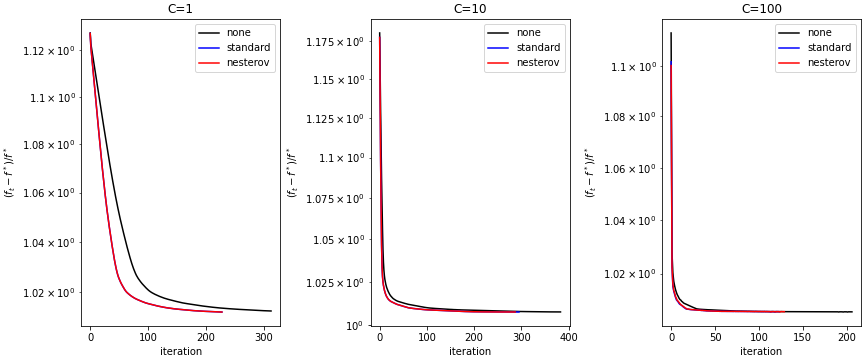
\includegraphics[scale=0.55]{img/l1_svc_loss_history}
	\caption{SGD Convergence for the Primal formulation of the $\protect \mathcal{L}_1$-SVC}
	\label{fig:l1_svc_history}
\end{figure}

\paragraph{Linear Dual formulations}

The experiments results shown in~\ref{linear_lagrangian_dual_l1_svc_cv_results} are obtained with $\alpha$, i.e., the \emph{learning rate} or \emph{step size}, setted to 1 for the \emph{AdaGrad} algorithm. Note that the \emph{unreg\_bias} and \emph{reg\_bias} duals refers to the augmented dual formulations~\eqref{eq:l1_svc_aug_lagrangian_dual} and~\eqref{eq:l1_svc_bcqp_aug_lagrangian_dual} respectively with $\rho$ equals to 1. The optimization process is stopped if the primal-dual weight vector does not change by at least $1\mathrm{e}{-6}$  between two consecutive iterations.

\begin{table}[H]
\centering
\caption{Wolfe Dual linear $\protect \mathcal{L}_1$-SVC results}
\label{linear_dual_l1_svc_cv_results}
\begin{tabular}{llrrrr}
\toprule
       &     &  fit\_time &  accuracy &  n\_iter &  n\_sv \\
solver & C &           &           &         &       \\
\midrule
smo & 1   &  0.073731 &     0.980 &      62 &    17 \\
       & 10  &  0.146260 &     0.980 &     295 &    10 \\
       & 100 &  0.160641 &     0.985 &     399 &     8 \\
libsvm & 1   &  0.003538 &     0.985 &     243 &    17 \\
       & 10  &  0.002517 &     0.985 &     194 &    10 \\
       & 100 &  0.002370 &     0.985 &    1602 &     8 \\
cvxopt & 1   &  0.033754 &     0.980 &      10 &    17 \\
       & 10  &  0.026945 &     0.980 &      10 &    11 \\
       & 100 &  0.047614 &     0.980 &      10 &    12 \\
\bottomrule
\end{tabular}
\end{table}


For what about the linear \emph{Wolfe dual} formulation we can immediately notice as higher \emph{regularization hyperparameter} $C$ makes the model harder, so the \emph{custom} implementation of the SMO algorithm and also the \emph{sklearn} implementation, i.e., \emph{libsvm}~\cite{chang2011libsvm} implementation, needs to perform more iterations to achieve the same \emph{numerical precision}; meanwhile the \emph{cvxopt}~\cite{vandenberghe2010cvxopt} seems to be insensitive to the increasing complexity of the model. The results in terms of \emph{accuracy} and number of \emph{support vectors} are strongly similar to each others.

\begin{table}[H]
\centering
\caption{Lagrangian Dual linear $\protect \mathcal{L}_1$-SVC results}
\label{linear_lagrangian_dual_l1_svc_cv_results}
\begin{tabular}{llrrrr}
\toprule
           &     &  fit\_time &  accuracy &  n\_iter &  n\_sv \\
dual & C &           &           &         &       \\
\midrule
reg\_bias & 1   &  0.012731 &     0.985 &       1 &   194 \\
           & 10  &  0.019405 &     0.985 &       1 &   194 \\
           & 100 &  0.030348 &     0.985 &       1 &   194 \\
unreg\_bias & 1   &  0.034859 &     0.985 &       1 &   196 \\
           & 10  &  0.030251 &     0.985 &       1 &   196 \\
           & 100 &  0.031609 &     0.985 &       1 &   196 \\
\bottomrule
\end{tabular}
\end{table}


For what about the linear \emph{Lagrangian dual} formulation we can see as it seems to be insensitive to the increasing complexity of the model in terms of number of \emph{iterations} but it tends to select many training data points as \emph{support vectors}.

\paragraph{Nonlinear Dual formulations}

The experiments results shown in~\ref{nonlinear_dual_l1_svc_cv_results} and~\ref{nonlinear_lagrangian_dual_l1_svc_cv_results} are obtained with \emph{d} and \emph{r} hyperparameters equal to 3 and 1 respectively for the \emph{polynomial} kernel; \emph{gamma} is setted to \emph{`scale`} for both \emph{polynomial} and \emph{gaussian} kernels. The experiments results shown in~\ref{nonlinear_lagrangian_dual_l1_svc_cv_results} are obtained with $\alpha$, i.e., the \emph{learning rate} or \emph{step size}, setted to 1 for the \emph{AdaGrad} algorithm. Note that the \emph{unreg\_bias} and \emph{reg\_bias} duals refers to the augmented dual formulations~\eqref{eq:l1_svc_aug_lagrangian_dual} and~\eqref{eq:l1_svc_bcqp_aug_lagrangian_dual} respectively with $\rho$ equals to 1. The optimization process is stopped if the primal-dual weight vector does not change by at least $1\mathrm{e}{-6}$  between two consecutive iterations.

\begin{table}[H]
\centering
\caption{Wolfe Dual nonlinear $\protect \mathcal{L}_1$-SVC results}
\label{nonlinear_dual_l1_svc_cv_results}
\begin{tabular}{lllrrrr}
\toprule
       &      &      &  fit\_time &  accuracy &  n\_iter &  n\_sv \\
solver & kernel & C &           &           &         &       \\
\midrule
smo & gaussian & 0.1  &  0.878962 &    1.0000 &      65 &   222 \\
       &      & 1.0  &  0.860773 &    1.0000 &      76 &    48 \\
       &      & 10.0 &  0.525582 &    1.0000 &      29 &    13 \\
       & poly & 0.1  &  1.096614 &    0.8675 &     121 &   142 \\
       &      & 1.0  &  0.999406 &    0.6825 &     143 &    30 \\
       &      & 10.0 &  0.680124 &    0.9475 &      65 &    10 \\
libsvm & gaussian & 0.1  &  0.011811 &    1.0000 &     131 &   222 \\
       &      & 1.0  &  0.007152 &    1.0000 &     252 &    50 \\
       &      & 10.0 &  0.003799 &    1.0000 &     134 &    13 \\
       & poly & 0.1  &  0.022929 &    1.0000 &     210 &   143 \\
       &      & 1.0  &  0.010823 &    1.0000 &     233 &    30 \\
       &      & 10.0 &  0.003304 &    1.0000 &     118 &    10 \\
cvxopt & gaussian & 0.1  &  0.426778 &    1.0000 &      10 &   222 \\
       &      & 1.0  &  0.568489 &    1.0000 &      10 &    49 \\
       &      & 10.0 &  0.557587 &    1.0000 &      10 &    14 \\
       & poly & 0.1  &  0.487677 &    0.8575 &      10 &   143 \\
       &      & 1.0  &  0.693849 &    0.6775 &      10 &    31 \\
       &      & 10.0 &  0.610578 &    0.9475 &      10 &    10 \\
\bottomrule
\end{tabular}
\end{table}


\begin{table}[H]
\centering
\caption{Lagrangian Dual nonlinear $\protect \mathcal{L}_1$-SVC results}
\label{nonlinear_lagrangian_dual_l1_svc_cv_results}
\begin{tabular}{lllrrrr}
\toprule
           &     &     &  fit\_time &  accuracy &  n\_iter &  n\_sv \\
dual & kernel & C &           &           &         &       \\
\midrule
reg\_bias & poly & 1   &  0.910125 &    0.6350 &     222 &   317 \\
           &     & 10  &  0.855964 &    0.6350 &     222 &   317 \\
           &     & 100 &  1.015074 &    0.6350 &     222 &   317 \\
           & rbf & 1   &  0.084307 &    1.0000 &       1 &   399 \\
           &     & 10  &  0.073900 &    1.0000 &       1 &   399 \\
           &     & 100 &  0.075157 &    1.0000 &       1 &   399 \\
unreg\_bias & poly & 1   &  0.069840 &    0.6075 &       3 &   314 \\
           &     & 10  &  0.068924 &    0.6075 &       3 &   314 \\
           &     & 100 &  0.058743 &    0.6075 &       3 &   314 \\
           & rbf & 1   &  0.117894 &    0.5000 &      11 &   115 \\
           &     & 10  &  0.359374 &    0.5575 &      46 &   282 \\
           &     & 100 &  0.385576 &    0.5575 &      46 &   282 \\
\bottomrule
\end{tabular}
\end{table}


The same considerations made for the previous linear \emph{Wolfe dual} and \emph{Lagrangian dual} formulations are confirmed also in the nonlinearly separable case. In this setting the complexity of the model coming with higher $C$ regularization values seems to be not paying a tradeoff in terms of the number of \emph{iterations} of the algorithm and, moreover, the \emph{reg\_bias Lagrangian dual} formulation seems to perform better wrt the \emph{unreg\_bias} formulation, both tends to select even more training data points as \emph{support vectors}.

\begin{figure}[H]
	\centering
	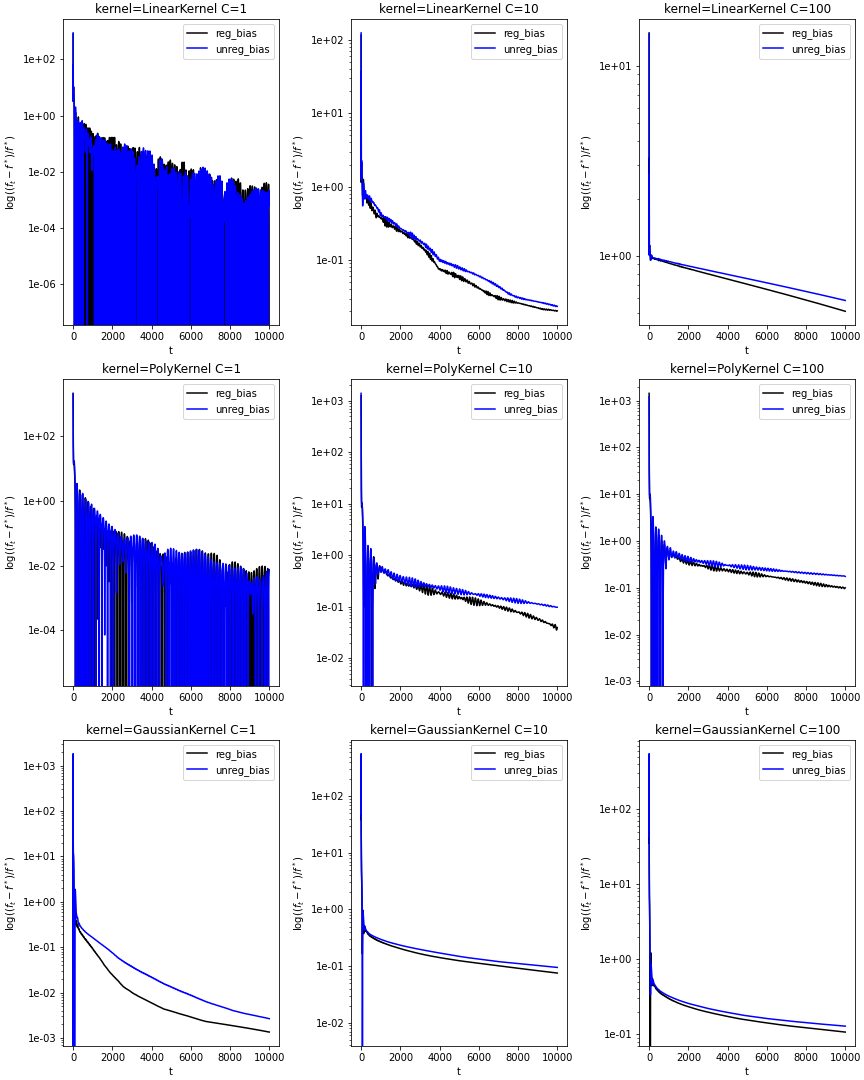
\includegraphics[scale=0.55]{img/lagrangian_dual_l1_svc_loss_history}
	\caption{AdaGrad convergence for the Lagrangian Dual formulation of the nonlinear $\protect \mathcal{L}_1$-SVC}
	\label{fig:lagrangian_dual_l1_svc_loss_history}
\end{figure}

\pagebreak

\subsubsection{Squared Hinge loss}

\paragraph{Primal formulation}

The experiments results shown in~\ref{primal_l2_svc_cv_results} referred to \emph{Stochastic Gradient Descent} algorithm are obtained with $\alpha$, i.e., the \emph{learning rate} or \emph{step size}, setted to 0.02 and $\beta$, i.e., the \emph{momentum}, equal to 0.5. The optimization process is stopped if after 5 iterations the function value does not improve by at least $1\mathrm{e}{-8}$.

\begin{table}[H]
\centering
\caption{SVC Primal formulation results with Squared Hinge loss}
\label{primal_l2_svc_cv_results}
\begin{tabular}{lllrrrr}
\toprule
          &   &     &  fit\_time &  accuracy &  n\_iter &  n\_sv \\
solver & momentum & C &           &           &         &       \\
\midrule
sgd & none & 1   &  0.419254 &     0.975 &     154 &    49 \\
          &   & 10  &  0.314466 &     0.980 &     119 &    24 \\
          &   & 100 &  0.079897 &     0.985 &      30 &    15 \\
          & standard & 1   &  0.312977 &     0.975 &     113 &    45 \\
          &   & 10  &  0.203847 &     0.980 &      73 &    24 \\
          &   & 100 &  0.061971 &     0.985 &      21 &    11 \\
          & nesterov & 1   &  0.328923 &     0.970 &     132 &    40 \\
          &   & 10  &  0.188573 &     0.980 &      71 &    23 \\
          &   & 100 &  0.073157 &     0.985 &      26 &    10 \\
liblinear & - & 1   &  0.002038 &     0.980 &     556 &    25 \\
          &   & 10  &  0.002624 &     0.980 &    1000 &    19 \\
          &   & 100 &  0.002467 &     0.980 &    1000 &    27 \\
\bottomrule
\end{tabular}
\end{table}


Again, the results provided from the \emph{custom} implementation, i.e., the SGD with different momentum settings, are strongly similar to those of \emph{sklearn} implementation, i.e., \emph{liblinear}~\cite{fan2008liblinear} implementation, in terms of \emph{accuracy} score. More training data points are selected as \emph{support vectors} from the SGD solver but it always requires even lower iterations, i.e., epochs, to achieve the same \emph{numerical precision}. \emph{Polyak} and \emph{Nesterov} momentums always perform lower iterations as expected from the theoretical analysis of the convergence rate.

\begin{figure}[H]
	\centering
	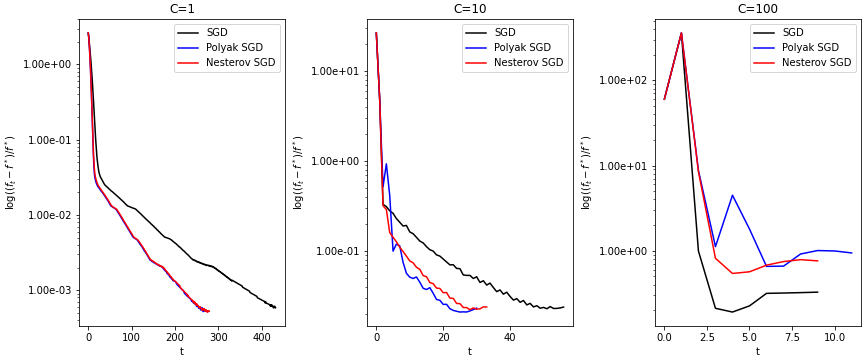
\includegraphics[scale=0.55]{img/l2_svc_loss_history}
	\caption{SGD convergence for the Primal formulation of the $\protect \mathcal{L}_2$-SVC}
	\label{fig:l2_svc_loss_history}
\end{figure}

\pagebreak

\paragraph{Linear Dual formulations}

The experiments results shown in~\ref{linear_lagrangian_dual_l2_svc_cv_results} are obtained with $\alpha$, i.e., the \emph{learning rate} or \emph{step size}, setted to 1 for the \emph{AdaGrad} algorithm. Note that the \emph{unreg\_bias} and \emph{reg\_bias} duals refers to the augmented dual formulations~\eqref{eq:l2_svc_aug_lagrangian_dual} and~\eqref{eq:l2_svc_lb_aug_lagrangian_dual} respectively with $\rho$ equals to 1. The optimization process is stopped if the primal-dual weight vector does not change by at least $1\mathrm{e}{-6}$  between two consecutive iterations.

\begin{table}[H]
\centering
\caption{Lagrangian Dual linear $\protect \mathcal{L}_2$-SVC results}
\label{linear_lagrangian_dual_l2_svc_cv_results}
\begin{tabular}{llrrrr}
\toprule
           &      &    fit\_time &  accuracy &  n\_iter &  n\_sv \\
dual & C &             &           &         &       \\
\midrule
reg\_bias & 0.1  &   14.878780 &     0.980 &    5146 &    50 \\
           & 1.0  &   66.392083 &     0.975 &   25316 &    29 \\
           & 10.0 &  268.694762 &     0.980 &   82805 &    19 \\
unreg\_bias & 0.1  &   16.323348 &     0.980 &    5363 &    51 \\
           & 1.0  &   69.190667 &     0.985 &   26362 &    31 \\
           & 10.0 &  254.510382 &     0.980 &   87850 &    19 \\
\bottomrule
\end{tabular}
\end{table}


For what about the linear \emph{Lagrangian dual} formulation we can see as it seems to be insensitive to the increasing complexity of the model in terms of number of \emph{iterations} but it tends to select many training data points as \emph{support vectors}.

\paragraph{Nonlinear Dual formulations}

The experiments results shown in~\ref{nonlinear_lagrangian_dual_l2_svc_cv_results} are obtained with \emph{d} and \emph{r} hyperparameters equal to 3 and 1 respectively for the \emph{polynomial} kernel; \emph{gamma} is setted to \emph{`scale`} for both \emph{polynomial} and \emph{gaussian} kernels. The experiments results shown in~\ref{nonlinear_lagrangian_dual_l1_svc_cv_results} are obtained with $\alpha$, i.e., the \emph{learning rate} or \emph{step size}, setted to 1 for the \emph{AdaGrad} algorithm. Note that the \emph{unreg\_bias} and \emph{reg\_bias} duals refers to the augmented dual formulations~\eqref{eq:l2_svc_aug_lagrangian_dual} and~\eqref{eq:l2_svc_lb_aug_lagrangian_dual} respectively with $\rho$ equals to 1. The optimization process is stopped if the primal-dual weight vector does not change by at least $1\mathrm{e}{-6}$  between two consecutive iterations.

\begin{table}[H]
\centering
\caption{Lagrangian Dual nonlinear $\protect \mathcal{L}_2$-SVC results}
\label{nonlinear_lagrangian_dual_l2_svc_cv_results}
\begin{tabular}{lllrrrr}
\toprule
           &     &      &    fit\_time &  accuracy &  n\_iter &  n\_sv \\
dual & kernel & C &             &           &         &       \\
\midrule
reg\_bias & poly & 0.1  &   31.788529 &    0.9025 &    8440 &   238 \\
           &     & 1.0  &  246.570286 &    0.9400 &   41399 &    90 \\
           &     & 10.0 &  511.538499 &    0.9800 &   71657 &    28 \\
           & rbf & 0.1  &    5.349926 &    1.0000 &    1376 &   353 \\
           &     & 1.0  &   47.321667 &    1.0000 &    9054 &   143 \\
           &     & 10.0 &  268.803593 &    1.0000 &   38253 &    33 \\
unreg\_bias & poly & 0.1  &   35.440141 &    0.9350 &    8820 &   241 \\
           &     & 1.0  &  256.988245 &    0.8925 &   44347 &    88 \\
           &     & 10.0 &  470.562703 &    1.0000 &   78511 &    25 \\
           & rbf & 0.1  &   10.977159 &    1.0000 &    2777 &   350 \\
           &     & 1.0  &   92.292312 &    1.0000 &   16319 &   143 \\
           &     & 10.0 &  310.204657 &    1.0000 &   59705 &    33 \\
\bottomrule
\end{tabular}
\end{table}


The same considerations made for the previous linear \emph{Lagrangian dual} formulations are confirmed also in the nonlinearly separable case. In this setting the complexity of the model coming with higher $C$ regularization values seems to be not paying a tradeoff in terms of the number of \emph{iterations} of the algorithm and, moreover, the \emph{reg\_bias Lagrangian dual} formulation seems to perform better wrt the \emph{unreg\_bias} formulation, both tends to select even more training data points as \emph{support vectors}.

\begin{figure}[H]
	\centering
	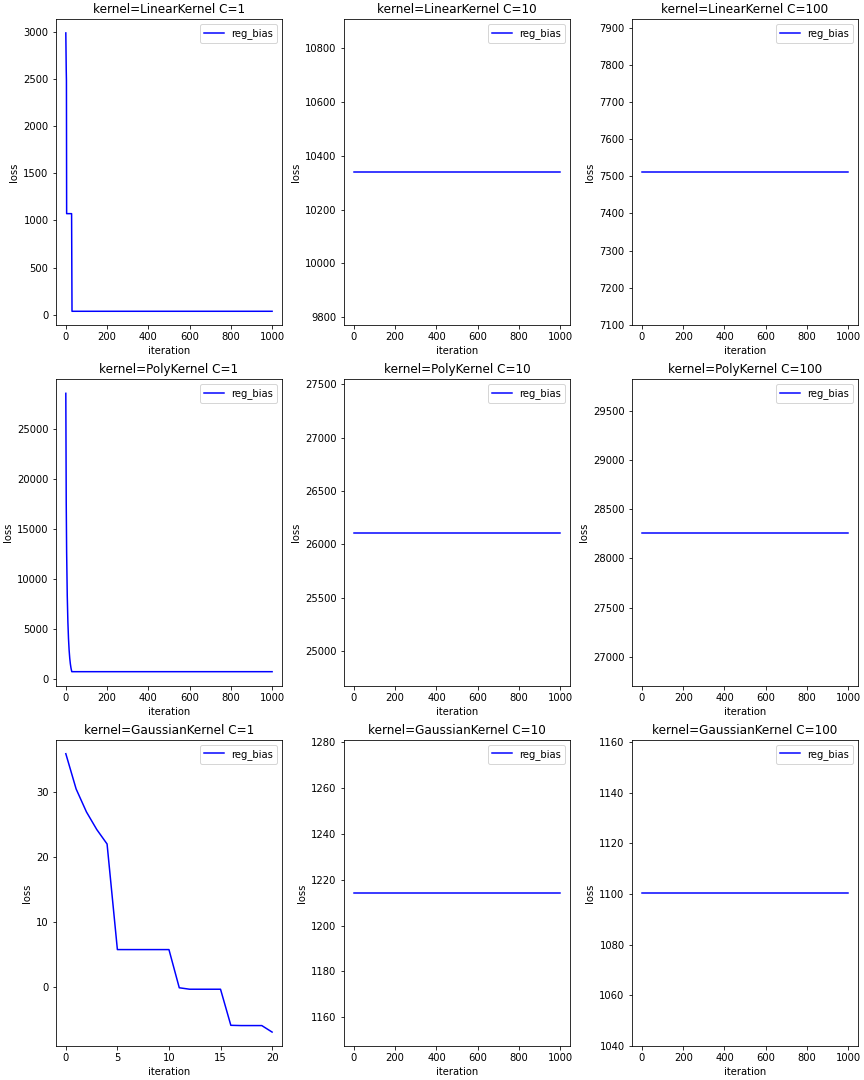
\includegraphics[scale=0.55]{img/lagrangian_dual_l2_svc_loss_history}
	\caption{AdaGrad convergence for the Lagrangian Dual formulation of the nonlinear $\protect \mathcal{L}_2$-SVC}
	\label{fig:lagrangian_dual_l2_svc_loss_history}
\end{figure}

\pagebreak

\subsection{Support Vector Regression}

Below experiments are about the SVR for which I tested different values for regularization hyperparameter $C$, i.e., from \emph{soft} to \emph{hard margin}, the $\epsilon$ penalty value and in case of nonlinearly separable data also different \emph{kernel functions} mentioned above.

The experiments about SVRs are available at: \\ \href{https://github.com/dmeoli/optiml/blob/master/notebooks/optimization/CM_SVR_report_experiments.ipynb}{\texttt{github.com/dmeoli/optiml/blob/master/notebooks/optimization/CM\_SVR\_report\_experiments.ipynb}}.

\subsubsection{Epsilon-insensitive loss}

\paragraph{Primal formulation}

The experiments results shown in~\ref{primal_l1_svr_cv_results} referred to \emph{Stochastic Gradient Descent} algorithm are obtained with $\alpha$, i.e., the \emph{learning rate} or \emph{step size}, setted to 0.02 and $\beta$, i.e., the \emph{momentum}, equal to 0.4. The optimization process is stopped if after 5 iterations the function value does not improve by at least $1\mathrm{e}{-8}$.

\begin{table}[H]
\centering
\caption{Primal $\protect \mathcal{L}_1$-SVR results}
\label{primal_l1_svr_cv_results}
\begin{tabular}{llllrrrr}
\toprule
          &   &     &     &   fit\_time &        r2 &  n\_iter &  n\_sv \\
solver & momentum & C & epsilon &            &           &         &       \\
\midrule
sgd & none & 1   & 0.1 &  13.207407 &  0.954298 &   16161 &   100 \\
          &   &     & 0.2 &   9.523358 &  0.954544 &   12267 &    99 \\
          &   &     & 0.3 &  11.594773 &  0.955424 &   13665 &    99 \\
          &   & 10  & 0.1 &   0.690761 &  0.983893 &     806 &    98 \\
          &   &     & 0.2 &   0.722907 &  0.983891 &     884 &    98 \\
          &   &     & 0.3 &   0.756686 &  0.983884 &     958 &    97 \\
          &   & 100 & 0.1 &   0.121053 &  0.984034 &      85 &    97 \\
          &   &     & 0.2 &   0.088140 &  0.984047 &      96 &    98 \\
          &   &     & 0.3 &   0.156799 &  0.984056 &     109 &    98 \\
          & polyak & 1   & 0.1 &   7.895537 &  0.954321 &    9874 &   100 \\
          &   &     & 0.2 &   5.816864 &  0.954549 &    7400 &    99 \\
          &   &     & 0.3 &   6.935173 &  0.955424 &    8200 &    99 \\
          &   & 10  & 0.1 &   0.489926 &  0.983893 &     487 &    97 \\
          &   &     & 0.2 &   0.503936 &  0.983891 &     535 &    98 \\
          &   &     & 0.3 &   0.483785 &  0.983885 &     569 &    98 \\
          &   & 100 & 0.1 &   0.090085 &  0.984030 &      48 &    98 \\
          &   &     & 0.2 &   0.108489 &  0.984046 &      56 &    98 \\
          &   &     & 0.3 &   0.114756 &  0.984055 &      61 &    97 \\
          & nesterov & 1   & 0.1 &   8.996545 &  0.954310 &    9785 &   100 \\
          &   &     & 0.2 &   6.001156 &  0.954546 &    7382 &    99 \\
          &   &     & 0.3 &   7.318327 &  0.955424 &    8198 &    99 \\
          &   & 10  & 0.1 &   0.803194 &  0.983892 &     489 &    97 \\
          &   &     & 0.2 &   0.457146 &  0.983890 &     533 &    97 \\
          &   &     & 0.3 &   0.561535 &  0.983884 &     579 &    98 \\
          &   & 100 & 0.1 &   0.097744 &  0.984031 &      61 &    98 \\
          &   &     & 0.2 &   0.120314 &  0.984047 &      58 &    98 \\
          &   &     & 0.3 &   0.107943 &  0.984057 &      62 &    98 \\
liblinear & - & 1   & 0.1 &   0.019717 &  0.954684 &      12 &   100 \\
          &   &     & 0.2 &   0.001534 &  0.955112 &      10 &    99 \\
          &   &     & 0.3 &   0.001302 &  0.955415 &      10 &    97 \\
          &   & 10  & 0.1 &   0.002194 &  0.983893 &      57 &    99 \\
          &   &     & 0.2 &   0.001483 &  0.983890 &      69 &    98 \\
          &   &     & 0.3 &   0.001968 &  0.983906 &     142 &    97 \\
          &   & 100 & 0.1 &   0.001972 &  0.984023 &     980 &    97 \\
          &   &     & 0.2 &   0.006431 &  0.984028 &    1340 &    97 \\
          &   &     & 0.3 &   0.002328 &  0.984051 &    2886 &    97 \\
\bottomrule
\end{tabular}
\end{table}


The results provided from the \emph{custom} implementation, i.e., the SGD with different momentum settings, are strongly similar to those of \emph{sklearn} implementation, i.e., \emph{liblinear}~\cite{fan2008liblinear} implementation, in terms of \emph{r2} score, except in case of $C$ regularization hyperparameter equals to 1 for which those of SGD are lower. Moreover, the SGD solver always requires lower iterations, i.e., epochs, for higher $C$ regularization values, i.e., for $C$ equals to 10 or 100, to achieve the same \emph{numerical precision}. Again, \emph{Polyak} and \emph{Nesterov} momentums always perform lower iterations as expected from the theoretical analysis of the convergence rate. The results in terms of \emph{support vectors} are strongly similar to each others.

\begin{figure}[H]
	\centering
	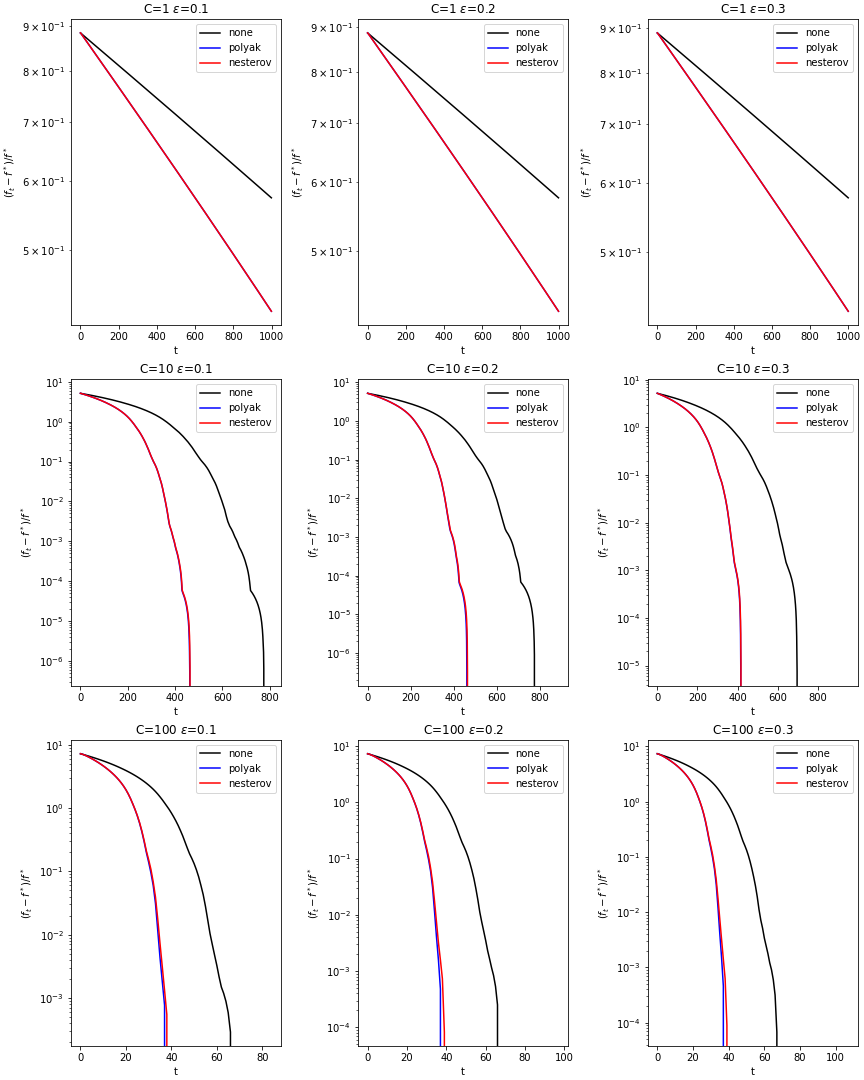
\includegraphics[scale=0.5]{img/l1_svr_loss_history}
	\caption{SGD convergence for the Primal formulation of the $\protect \mathcal{L}_1$-SVR}
	\label{fig:l1_svr_loss_history}
\end{figure}

\pagebreak

\paragraph{Linear Dual formulations}

The experiments results shown in~\ref{linear_lagrangian_dual_l1_svr_cv_results} are obtained with $\alpha$, i.e., the \emph{learning rate} or \emph{step size}, setted to 1 for the \emph{AdaGrad} algorithm. Note that the \emph{unreg\_bias} and \emph{reg\_bias} duals refers to the augmented dual formulations~\eqref{eq:l1_svr_aug_lagrangian_dual} and~\eqref{eq:l1_svr_bcqp_aug_lagrangian_dual} respectively with $\rho$ equals to 1. The optimization process is stopped if the primal-dual weight vector does not change by at least $1\mathrm{e}{-6}$  between two consecutive iterations.

\begin{table}[H]
\centering
\caption{Wolfe Dual linear $\protect \mathcal{L}_1$-SVR results}
\label{linear_dual_l1_svr_cv_results}
\begin{tabular}{lllrrrr}
\toprule
       &     &     &  fit\_time &        r2 &  n\_iter &  n\_sv \\
solver & C & epsilon &           &           &         &       \\
\midrule
smo & 1   & 0.1 &  0.049352 &  0.954396 &      10 &   100 \\
       &     & 0.2 &  0.026155 &  0.954546 &      15 &   100 \\
       &     & 0.3 &  0.090050 &  0.955429 &      13 &    99 \\
       & 10  & 0.1 &  0.201986 &  0.983893 &      44 &    99 \\
       &     & 0.2 &  0.091500 &  0.983893 &      48 &    99 \\
       &     & 0.3 &  0.084329 &  0.983893 &      41 &    99 \\
       & 100 & 0.1 &  0.826075 &  0.984071 &     623 &    98 \\
       &     & 0.2 &  0.409304 &  0.984088 &     157 &    98 \\
       &     & 0.3 &  0.521488 &  0.984103 &     334 &    98 \\
libsvm & 1   & 0.1 &  0.009594 &  0.954393 &      79 &   100 \\
       &     & 0.2 &  0.005095 &  0.954543 &      82 &   100 \\
       &     & 0.3 &  0.029558 &  0.955424 &      78 &    99 \\
       & 10  & 0.1 &  0.033350 &  0.983892 &     206 &    99 \\
       &     & 0.2 &  0.005173 &  0.983890 &     219 &    99 \\
       &     & 0.3 &  0.009250 &  0.983885 &     216 &    99 \\
       & 100 & 0.1 &  0.019970 &  0.984028 &    2239 &    98 \\
       &     & 0.2 &  0.006288 &  0.984041 &    1189 &    98 \\
       &     & 0.3 &  0.003961 &  0.984051 &    1366 &    98 \\
cvxopt & 1   & 0.1 &  0.122198 &  0.954685 &       9 &   100 \\
       &     & 0.2 &  0.152970 &  0.954849 &       9 &   100 \\
       &     & 0.3 &  0.066905 &  0.955429 &      10 &   100 \\
       & 10  & 0.1 &  0.144911 &  0.983893 &       9 &   100 \\
       &     & 0.2 &  0.056698 &  0.983893 &       8 &   100 \\
       &     & 0.3 &  0.045109 &  0.983893 &       8 &   100 \\
       & 100 & 0.1 &  0.094987 &  0.984071 &       9 &   100 \\
       &     & 0.2 &  0.070957 &  0.984088 &       9 &   100 \\
       &     & 0.3 &  0.095619 &  0.984103 &       8 &   100 \\
\bottomrule
\end{tabular}
\end{table}


For what about the linear \emph{Wolfe dual} formulation we can immediately notice as higher \emph{regularization hyperparameter} $C$ and lower $\epsilon$ values makes the model harder, so the \emph{custom} implementation of the SMO algorithm and also the \emph{sklearn} implementation, i.e., \emph{libsvm}~\cite{chang2011libsvm} implementation, needs to perform more iterations to achieve the same \emph{numerical precision}; meanwhile, again, the \emph{cvxopt}~\cite{vandenberghe2010cvxopt} seems to be insensitive to the increasing complexity of the model. The results in terms of \emph{r2} and number of \emph{support vectors} are strongly similar to each others.

\begin{table}[H]
\centering
\caption{Lagrangian Dual linear $\protect \mathcal{L}_1$-SVR results}
\label{linear_lagrangian_dual_l1_svr_cv_results}
\begin{tabular}{lllrrrr}
\toprule
           &     &     &    fit\_time &        r2 &  n\_iter &  n\_sv \\
dual & C & epsilon &             &           &         &       \\
\midrule
reg\_bias & 1   & 0.1 &   23.881113 &  0.954685 &   22445 &   100 \\
           &     & 0.2 &   31.481934 &  0.954845 &   22235 &   100 \\
           &     & 0.3 &   24.310760 &  0.955429 &   21493 &    99 \\
           & 10  & 0.1 &   43.878878 &  0.983893 &   24700 &    99 \\
           &     & 0.2 &   43.092336 &  0.983893 &   26586 &    99 \\
           &     & 0.3 &   60.609057 &  0.983893 &   26076 &    99 \\
           & 100 & 0.1 &  151.873868 &  0.984071 &  105273 &    98 \\
           &     & 0.2 &  173.833673 &  0.984088 &  141626 &    98 \\
           &     & 0.3 &  259.661015 &  0.984103 &  284365 &    98 \\
unreg\_bias & 1   & 0.1 &   49.656317 &  0.954396 &   24597 &   100 \\
           &     & 0.2 &   83.297098 &  0.954546 &   62678 &   100 \\
           &     & 0.3 &  313.268643 &  0.955429 &  332397 &    99 \\
           & 10  & 0.1 &   67.435317 &  0.983893 &   55824 &    99 \\
           &     & 0.2 &   85.381756 &  0.983893 &   56708 &    99 \\
           &     & 0.3 &  100.468285 &  0.983893 &   62786 &    99 \\
           & 100 & 0.1 &  675.775826 &  0.984071 &  491963 &    98 \\
           &     & 0.2 &  636.590656 &  0.984088 &  541088 &    98 \\
           &     & 0.3 &  634.562593 &  0.984103 &  674048 &    98 \\
\bottomrule
\end{tabular}
\end{table}


For what about the linear \emph{Lagrangian dual} formulation we can see as it seems to be insensitive to the increasing complexity of the model in terms of number of \emph{iterations} and require many \emph{iterations} wrt the \emph{Wolfe dual} formulation.

\begin{figure}[H]
	\centering
	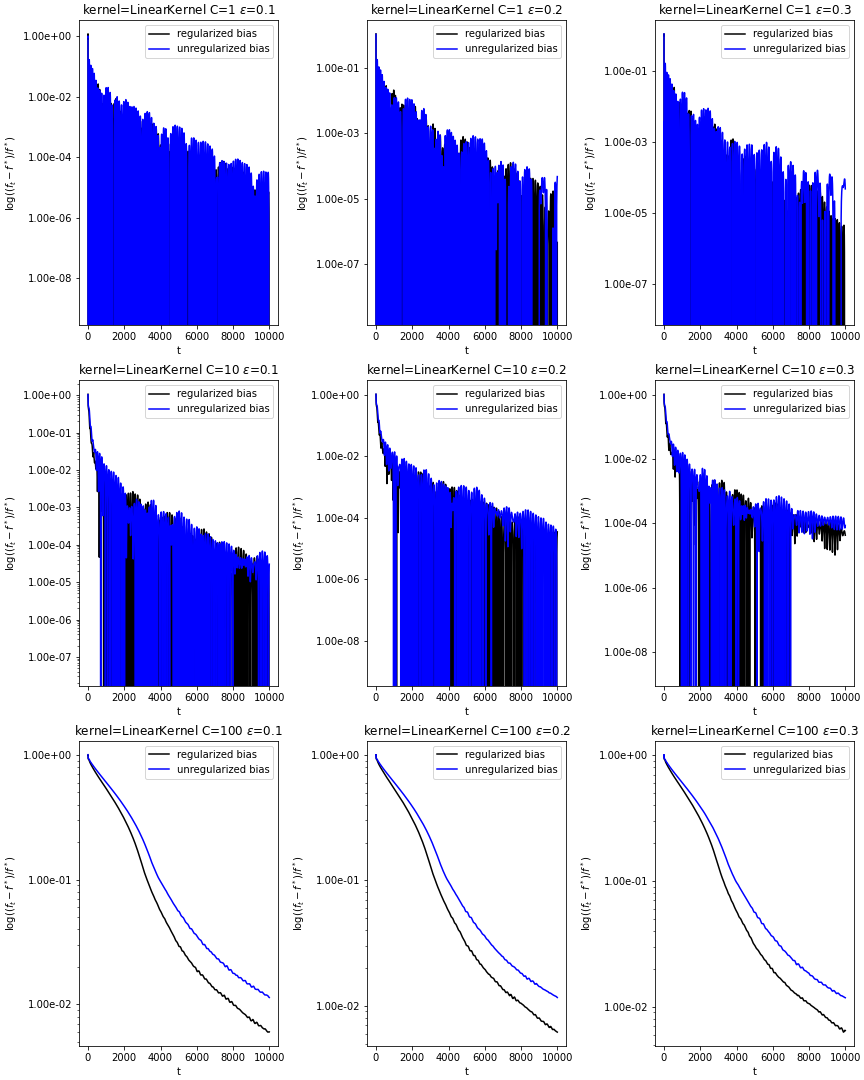
\includegraphics[scale=0.55]{img/linear_lagrangian_dual_l1_svr_loss_history}
	\caption{AdaGrad convergence for the Lagrangian Dual formulation of the linear $\protect \mathcal{L}_1$-SVR}
	\label{fig:linear_lagrangian_dual_l1_svr_loss_history}
\end{figure}

\paragraph{Nonlinear Dual formulations}

The experiments results shown in~\ref{nonlinear_dual_l1_svr_cv_results} and~\ref{nonlinear_lagrangian_dual_l1_svr_cv_results} are obtained with \emph{d} and \emph{r} hyperparameters both equal to 3 for the \emph{polynomial} kernel; \emph{gamma} is setted to \emph{`scale`} for both \emph{gaussian} and \emph{laplacian} kernels. The experiments results shown in~\ref{nonlinear_lagrangian_dual_l1_svc_cv_results} are obtained with $\alpha$, i.e., the \emph{learning rate} or \emph{step size}, setted to 1 for the \emph{AdaGrad} algorithm. Note that the \emph{unreg\_bias} and \emph{reg\_bias} duals refers to the augmented dual formulations~\eqref{eq:l1_svr_aug_lagrangian_dual} and~\eqref{eq:l1_svr_bcqp_aug_lagrangian_dual} respectively with $\rho$ equals to 1. The optimization process is stopped if the primal-dual weight vector does not change by at least $1\mathrm{e}{-6}$  between two consecutive iterations.

\begin{table}[H]
\centering
\caption{Wolfe Dual nonlinear $\protect \mathcal{L}_1$-SVR formulation results}
\label{nonlinear_dual_l1_svr_cv_results}
\begin{tabular}{llllrrrr}
\toprule
       &     &     &     &     fit\_time &        r2 &    n\_iter &  n\_sv \\
solver & kernel & C & epsilon &              &           &           &       \\
\midrule
smo & poly & 1   & 0.1 &    71.647312 &  0.810056 &     47694 &    36 \\
       &     &     & 0.2 &    12.618369 &  0.671256 &      8702 &     6 \\
       &     &     & 0.3 &     4.557922 &  0.302709 &      3654 &     4 \\
       &     & 10  & 0.1 &   318.425233 &  0.736098 &    256531 &    32 \\
       &     &     & 0.2 &    39.047974 &  0.923152 &     32629 &     4 \\
       &     &     & 0.3 &     4.677411 &  0.302709 &      3654 &     4 \\
       &     & 100 & 0.1 &  2086.026956 &  0.635585 &   3294613 &    33 \\
       &     &     & 0.2 &    40.670991 &  0.923152 &     32629 &     4 \\
       &     &     & 0.3 &     4.617724 &  0.302709 &      3654 &     4 \\
       & rbf & 1   & 0.1 &     0.054718 &  0.988244 &        66 &    17 \\
       &     &     & 0.2 &     0.018531 &  0.924292 &        20 &     7 \\
       &     &     & 0.3 &     0.016346 &  0.883022 &        17 &     5 \\
       &     & 10  & 0.1 &     0.440781 &  0.989739 &       389 &    18 \\
       &     &     & 0.2 &     0.027589 &  0.924995 &        25 &     6 \\
       &     &     & 0.3 &     0.007014 &  0.882816 &        11 &     5 \\
       &     & 100 & 0.1 &     3.799744 &  0.974756 &      6664 &    19 \\
       &     &     & 0.2 &     0.024482 &  0.924995 &        25 &     6 \\
       &     &     & 0.3 &     0.011137 &  0.882816 &        11 &     5 \\
libsvm & poly & 1   & 0.1 &     0.049065 &  0.981438 &    155092 &    37 \\
       &     &     & 0.2 &     0.015740 &  0.976358 &      7326 &     6 \\
       &     &     & 0.3 &     0.004452 &  0.951282 &      3969 &     4 \\
       &     & 10  & 0.1 &     0.166962 &  0.981769 &    578347 &    32 \\
       &     &     & 0.2 &     0.019647 &  0.979414 &     28452 &     4 \\
       &     &     & 0.3 &     0.004198 &  0.951282 &      3969 &     4 \\
       &     & 100 & 0.1 &     2.349179 &  0.981844 &  13306191 &    35 \\
       &     &     & 0.2 &     0.009665 &  0.979414 &     28452 &     4 \\
       &     &     & 0.3 &     0.012851 &  0.951282 &      3969 &     4 \\
       & rbf & 1   & 0.1 &     0.005776 &  0.990088 &        96 &    17 \\
       &     &     & 0.2 &     0.020616 &  0.977763 &        36 &     7 \\
       &     &     & 0.3 &     0.001456 &  0.945601 &        24 &     5 \\
       &     & 10  & 0.1 &     0.002339 &  0.990493 &       616 &    18 \\
       &     &     & 0.2 &     0.010448 &  0.980673 &        39 &     6 \\
       &     &     & 0.3 &     0.007578 &  0.945601 &        24 &     5 \\
       &     & 100 & 0.1 &     0.005937 &  0.990496 &      9854 &    18 \\
       &     &     & 0.2 &     0.008988 &  0.980673 &        39 &     6 \\
       &     &     & 0.3 &     0.002329 &  0.945601 &        24 &     5 \\
cvxopt & poly & 1   & 0.1 &     0.065255 &  0.828482 &        10 &    37 \\
       &     &     & 0.2 &     0.041122 &  0.666571 &        10 &     6 \\
       &     &     & 0.3 &     0.029873 &  0.350876 &         9 &     4 \\
       &     & 10  & 0.1 &     0.048030 &  0.629433 &        10 &    33 \\
       &     &     & 0.2 &     0.064068 &  0.928477 &        10 &     4 \\
       &     &     & 0.3 &     0.063453 &  0.350873 &        10 &     4 \\
       &     & 100 & 0.1 &     0.063773 &  0.712681 &        10 &    36 \\
       &     &     & 0.2 &     0.097430 &  0.928478 &        10 &     4 \\
       &     &     & 0.3 &     0.072250 &  0.350876 &        10 &     4 \\
       & rbf & 1   & 0.1 &     0.039900 &  0.988117 &        10 &    17 \\
       &     &     & 0.2 &     0.030282 &  0.924679 &        10 &     7 \\
       &     &     & 0.3 &     0.047886 &  0.883386 &        10 &     5 \\
       &     & 10  & 0.1 &     0.022933 &  0.989956 &        10 &    18 \\
       &     &     & 0.2 &     0.022819 &  0.925595 &        10 &     6 \\
       &     &     & 0.3 &     0.032468 &  0.883386 &        10 &     5 \\
       &     & 100 & 0.1 &     0.022127 &  0.990216 &        10 &    40 \\
       &     &     & 0.2 &     0.037909 &  0.925595 &        10 &     6 \\
       &     &     & 0.3 &     0.029582 &  0.883386 &        10 &     5 \\
\bottomrule
\end{tabular}
\end{table}


\begin{table}[H]
\centering
\caption{Lagrangian Dual nonlinear $\protect \mathcal{L}_1$-SVR results}
\label{nonlinear_lagrangian_dual_l1_svr_cv_results}
\begin{tabular}{llllrrrr}
\toprule
           &     &     &     &   fit\_time &        r2 &  n\_iter &  n\_sv \\
dual & kernel & C & epsilon &            &           &         &       \\
\midrule
reg\_bias & poly & 1   & 0.1 &   9.014323 &  0.980130 &   10000 &   100 \\
           &     &     & 0.2 &   7.949212 &  0.978522 &   10000 &   100 \\
           &     &     & 0.3 &   8.145561 &  0.975487 &   10000 &    99 \\
           &     & 10  & 0.1 &   8.056295 &  0.975741 &   10000 &   100 \\
           &     &     & 0.2 &   7.586514 &  0.965786 &   10000 &   100 \\
           &     &     & 0.3 &   7.546005 &  0.954454 &   10000 &   100 \\
           &     & 100 & 0.1 &   8.766536 &  0.975741 &   10000 &   100 \\
           &     &     & 0.2 &   7.580433 &  0.965786 &   10000 &   100 \\
           &     &     & 0.3 &   7.518447 &  0.954454 &   10000 &   100 \\
           & rbf & 1   & 0.1 &   9.239836 &  0.983938 &   10000 &    49 \\
           &     &     & 0.2 &   9.088686 &  0.977767 &   10000 &    17 \\
           &     &     & 0.3 &   9.433860 &  0.944901 &   10000 &    58 \\
           &     & 10  & 0.1 &   9.681272 &  0.988661 &   10000 &    37 \\
           &     &     & 0.2 &   8.926462 &  0.985573 &   10000 &    38 \\
           &     &     & 0.3 &   9.579983 &  0.938212 &   10000 &    37 \\
           &     & 100 & 0.1 &   9.050977 &  0.988661 &   10000 &    37 \\
           &     &     & 0.2 &   9.211919 &  0.985573 &   10000 &    38 \\
           &     &     & 0.3 &  10.618364 &  0.938212 &   10000 &    37 \\
unreg\_bias & poly & 1   & 0.1 &   8.242731 &  0.980066 &   10000 &   100 \\
           &     &     & 0.2 &   7.870472 &  0.977327 &   10000 &   100 \\
           &     &     & 0.3 &   7.946662 &  0.976209 &   10000 &   100 \\
           &     & 10  & 0.1 &   7.509824 &  0.976242 &   10000 &   100 \\
           &     &     & 0.2 &   7.686515 &  0.969756 &   10000 &   100 \\
           &     &     & 0.3 &   7.510774 &  0.952895 &   10000 &   100 \\
           &     & 100 & 0.1 &   7.761488 &  0.976242 &   10000 &   100 \\
           &     &     & 0.2 &   7.630195 &  0.969756 &   10000 &   100 \\
           &     &     & 0.3 &   7.696242 &  0.952895 &   10000 &   100 \\
           & rbf & 1   & 0.1 &   9.121422 &  0.989997 &   10000 &    98 \\
           &     &     & 0.2 &   9.455734 &  0.977496 &   10000 &    57 \\
           &     &     & 0.3 &   9.615668 &  0.938677 &   10000 &    85 \\
           &     & 10  & 0.1 &   9.210732 &  0.989394 &   10000 &    83 \\
           &     &     & 0.2 &   9.280972 &  0.977514 &   10000 &    53 \\
           &     &     & 0.3 &   9.276510 &  0.939582 &   10000 &    67 \\
           &     & 100 & 0.1 &   8.975165 &  0.989394 &   10000 &    83 \\
           &     &     & 0.2 &   9.288849 &  0.977514 &   10000 &    53 \\
           &     &     & 0.3 &   8.827427 &  0.939582 &   10000 &    67 \\
\bottomrule
\end{tabular}
\end{table}


The same considerations made for the previous linear \emph{Wolfe dual} and \emph{Lagrangian dual} formulations are confirmed also in the nonlinearly separable case. In this setting, the complexity of the model coming with higher $C$ regularization hyperparameters and lower $\epsilon$ values pays a larger tradeoff in terms of the number of \emph{iterations} of the algorithm.

\begin{figure}[H]
	\centering
	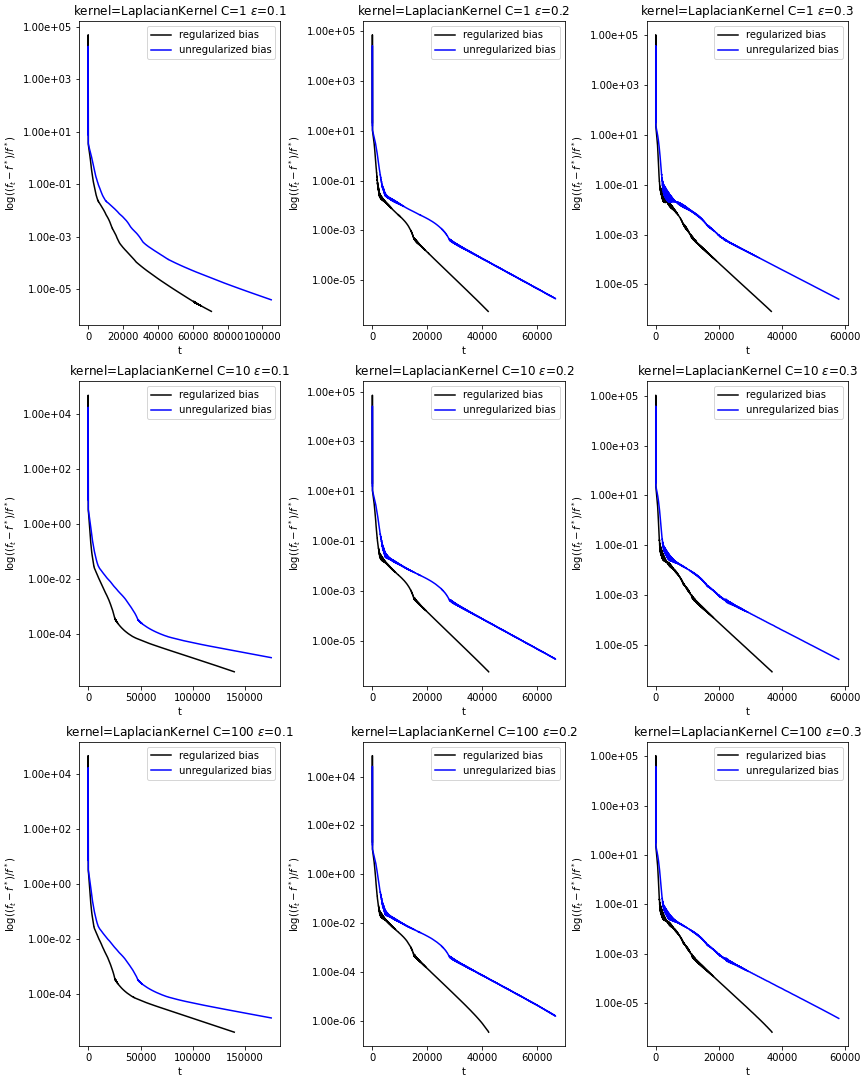
\includegraphics[scale=0.55]{img/laplacian_lagrangian_dual_l1_svr_loss_history}
	\caption{AdaGrad convergence for the Lagrangian Dual formulation of the Laplacian $\protect \mathcal{L}_1$-SVR}
	\label{fig:laplacian_lagrangian_dual_l1_svr_loss_history}
\end{figure}

\begin{figure}[H]
	\centering
	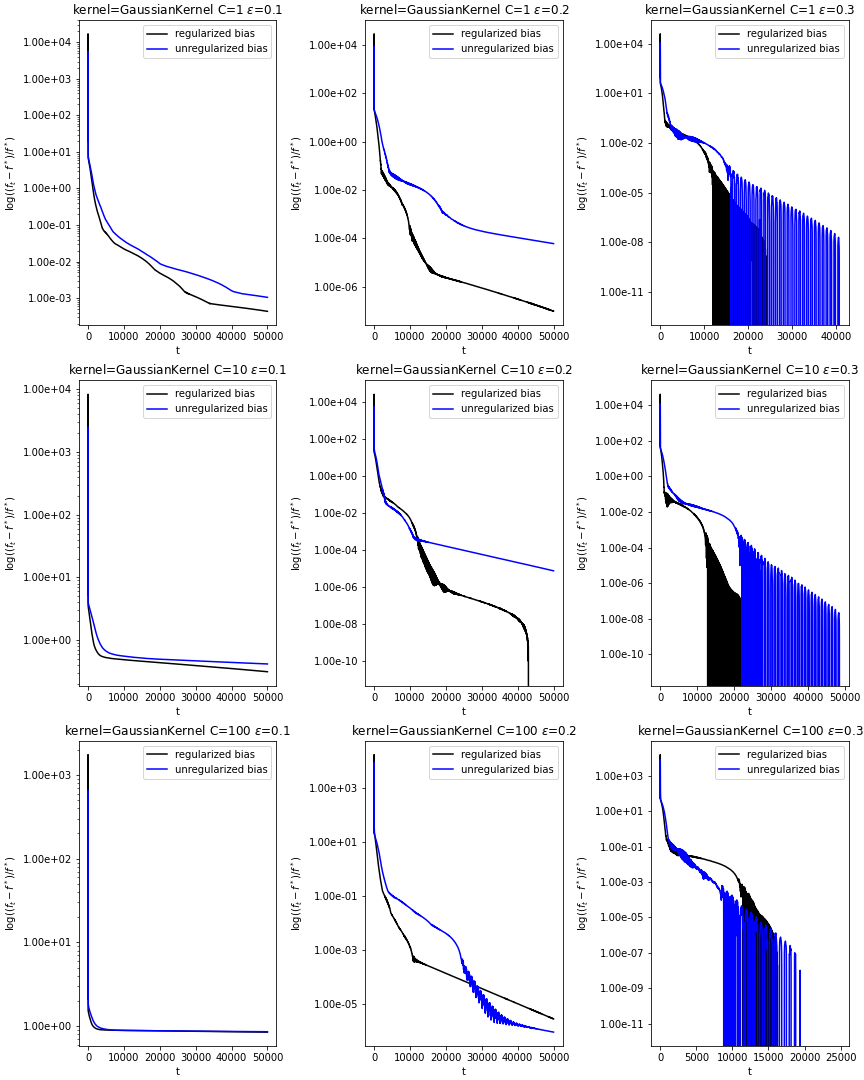
\includegraphics[scale=0.55]{img/gaussian_lagrangian_dual_l1_svr_loss_history}
	\caption{AdaGrad convergence for the Lagrangian Dual formulation of the Gaussian $\protect \mathcal{L}_1$-SVR}
	\label{fig:gaussian_lagrangian_dual_l1_svr_loss_history}
\end{figure}

\pagebreak

\subsubsection{Squared Epsilon-insensitive loss}

\paragraph{Primal formulation}

The experiments results shown in~\ref{primal_l2_svr_cv_results} referred to \emph{Stochastic Gradient Descent} algorithm are obtained with $\alpha$, i.e., the \emph{learning rate} or \emph{step size}, setted to 0.02 and $\beta$, i.e., the \emph{momentum}, equal to 0.4. The optimization process is stopped if after 5 iterations the function value does not improve by at least $1\mathrm{e}{-8}$.

\begin{table}[H]
\centering
\caption{Primal $\protect \mathcal{L}_2$-SVR results}
\label{primal_l2_svr_cv_results}
\begin{tabular}{llllrrrr}
\toprule
          &   &     &     &  fit\_time &        r2 &  n\_iter &  n\_sv \\
solver & momentum & C & epsilon &           &           &         &       \\
\midrule
sgd & none & 1   & 0.1 &  0.628824 &  0.977019 &     652 &   100 \\
          &   &     & 0.2 &  0.604419 &  0.977008 &     655 &    99 \\
          &   &     & 0.3 &  0.594717 &  0.976996 &     657 &    99 \\
          &   & 10  & 0.1 &  0.069660 &  0.977572 &      75 &    99 \\
          &   &     & 0.2 &  0.069005 &  0.977572 &      75 &    99 \\
          &   &     & 0.3 &  0.070856 &  0.977571 &      76 &    99 \\
          &   & 100 & 0.1 &  0.008819 &  0.977413 &       8 &   100 \\
          &   &     & 0.2 &  0.009804 &  0.977418 &       9 &    99 \\
          &   &     & 0.3 &  0.009794 &  0.977423 &       9 &    98 \\
          & standard & 1   & 0.1 &  0.397914 &  0.977028 &     405 &   100 \\
          &   &     & 0.2 &  0.371360 &  0.977018 &     407 &    99 \\
          &   &     & 0.3 &  0.379346 &  0.977006 &     408 &    99 \\
          &   & 10  & 0.1 &  0.040419 &  0.977572 &      42 &    99 \\
          &   &     & 0.2 &  0.043567 &  0.977571 &      42 &    99 \\
          &   &     & 0.3 &  0.041749 &  0.977571 &      43 &    99 \\
          &   & 100 & 0.1 &  0.007162 &  0.977443 &       6 &    99 \\
          &   &     & 0.2 &  0.006814 &  0.977447 &       6 &    99 \\
          &   &     & 0.3 &  0.007255 &  0.977450 &       6 &    97 \\
          & nesterov & 1   & 0.1 &  0.403233 &  0.977028 &     406 &   100 \\
          &   &     & 0.2 &  0.376248 &  0.977018 &     408 &    99 \\
          &   &     & 0.3 &  0.379239 &  0.977006 &     409 &    99 \\
          &   & 10  & 0.1 &  0.040307 &  0.977572 &      43 &    99 \\
          &   &     & 0.2 &  0.043603 &  0.977571 &      43 &    99 \\
          &   &     & 0.3 &  0.041826 &  0.977570 &      43 &    99 \\
          &   & 100 & 0.1 &  0.007321 &  0.977417 &       6 &   100 \\
          &   &     & 0.2 &  0.007085 &  0.977423 &       6 &    99 \\
          &   &     & 0.3 &  0.007221 &  0.977428 &       6 &    98 \\
liblinear & - & 1   & 0.1 &  0.000905 &  0.977554 &      96 &   100 \\
          &   &     & 0.2 &  0.001104 &  0.977553 &      96 &   100 \\
          &   &     & 0.3 &  0.001333 &  0.977551 &      96 &   100 \\
          &   & 10  & 0.1 &  0.003077 &  0.977577 &     826 &   100 \\
          &   &     & 0.2 &  0.003161 &  0.977576 &     826 &    99 \\
          &   &     & 0.3 &  0.003165 &  0.977576 &     839 &    99 \\
          &   & 100 & 0.1 &  0.003899 &  0.977538 &    1000 &   100 \\
          &   &     & 0.2 &  0.003790 &  0.977540 &    1000 &    99 \\
          &   &     & 0.3 &  0.004260 &  0.977541 &    1000 &    98 \\
\bottomrule
\end{tabular}
\end{table}


Again, the results provided from the \emph{custom} implementation, i.e., the SGD with different momentum settings, are strongly similar to those of \emph{sklearn} implementation, i.e., \emph{liblinear}~\cite{fan2008liblinear} implementation, in terms of \emph{r2} score. SGD solver always requires even lower iterations, i.e., epochs, for higher $C$ regularization values, i.e., for $C$ equals to 10 or 100, to achieve the same \emph{numerical precision}. \emph{Polyak} and \emph{Nesterov} momentums always perform lower iterations as expected from the theoretical analysis of the convergence rate.

\begin{figure}[H]
	\centering
	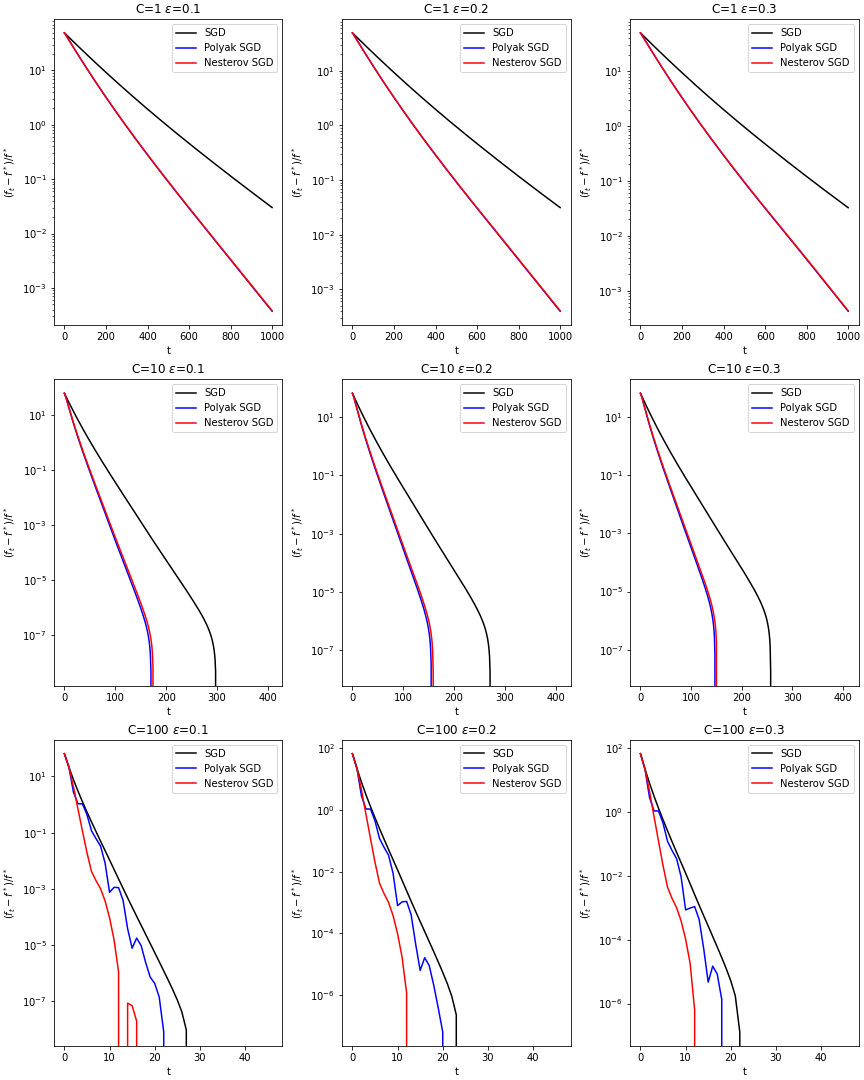
\includegraphics[scale=0.5]{img/l2_svr_loss_history}
	\caption{SGD convergence for the Primal formulation of the $\protect \mathcal{L}_2$-SVR}
	\label{fig:l2_svr_loss_history}
\end{figure}

\pagebreak

\paragraph{Linear Dual formulations}

The experiments results shown in~\ref{linear_lagrangian_dual_l2_svr_cv_results} are obtained with $\alpha$, i.e., the \emph{learning rate} or \emph{step size}, setted to 1 for the \emph{AdaGrad} algorithm. Note that the \emph{unreg\_bias} and \emph{reg\_bias} duals refers to the augmented dual formulations~\eqref{eq:l2_svr_aug_lagrangian_dual} and~\eqref{eq:l2_svr_lb_aug_lagrangian_dual} respectively with $\rho$ equals to 1. The optimization process is stopped if the primal-dual weight vector does not change by at least $1\mathrm{e}{-6}$  between two consecutive iterations.

\begin{table}[H]
\centering
\caption{Lagrangian Dual linear $\protect \mathcal{L}_2$-SVR results}
\label{linear_lagrangian_dual_l2_svr_cv_results}
\begin{tabular}{lllrrrr}
\toprule
           &     &     &      fit\_time &        r2 &    n\_iter &  n\_sv \\
dual & C & epsilon &               &           &           &       \\
\midrule
reg\_bias & 1   & 0.1 &      5.964492 &  0.984109 &      8402 &   100 \\
           &     & 0.2 &      6.434380 &  0.984109 &      8401 &   100 \\
           &     & 0.3 &      6.194610 &  0.984109 &      8351 &    98 \\
           & 10  & 0.1 &    127.675172 &  0.984133 &    158138 &    98 \\
           &     & 0.2 &    123.495917 &  0.984133 &    157026 &    98 \\
           &     & 0.3 &    123.505926 &  0.984133 &    155918 &    98 \\
           & 100 & 0.1 &   8652.729938 &  0.984133 &  10694001 &    98 \\
           &     & 0.2 &  10317.446609 &  0.984133 &  10606543 &    98 \\
           &     & 0.3 &  12464.591213 &  0.984133 &  10519497 &    98 \\
unreg\_bias & 1   & 0.1 &      6.708170 &  0.984109 &      9353 &   100 \\
           &     & 0.2 &      6.801255 &  0.984109 &      9292 &   100 \\
           &     & 0.3 &      8.526457 &  0.984109 &      9300 &    98 \\
           & 10  & 0.1 &    136.818768 &  0.984133 &    172114 &    98 \\
           &     & 0.2 &    137.433034 &  0.984133 &    170997 &    98 \\
           &     & 0.3 &    136.082049 &  0.984133 &    169887 &    98 \\
           & 100 & 0.1 &   8646.371154 &  0.984133 &  10814009 &    98 \\
           &     & 0.2 &  11637.626876 &  0.984133 &  10726702 &    98 \\
           &     & 0.3 &  14121.175771 &  0.984133 &  10639827 &    98 \\
\bottomrule
\end{tabular}
\end{table}


For what about the linear \emph{Lagrangian dual} formulation we can see as it seems to be insensitive to the increasing complexity of the model in terms of number of \emph{iterations} and require many \emph{iterations} wrt the \emph{Wolfe dual} formulation.

\begin{figure}[H]
	\centering
	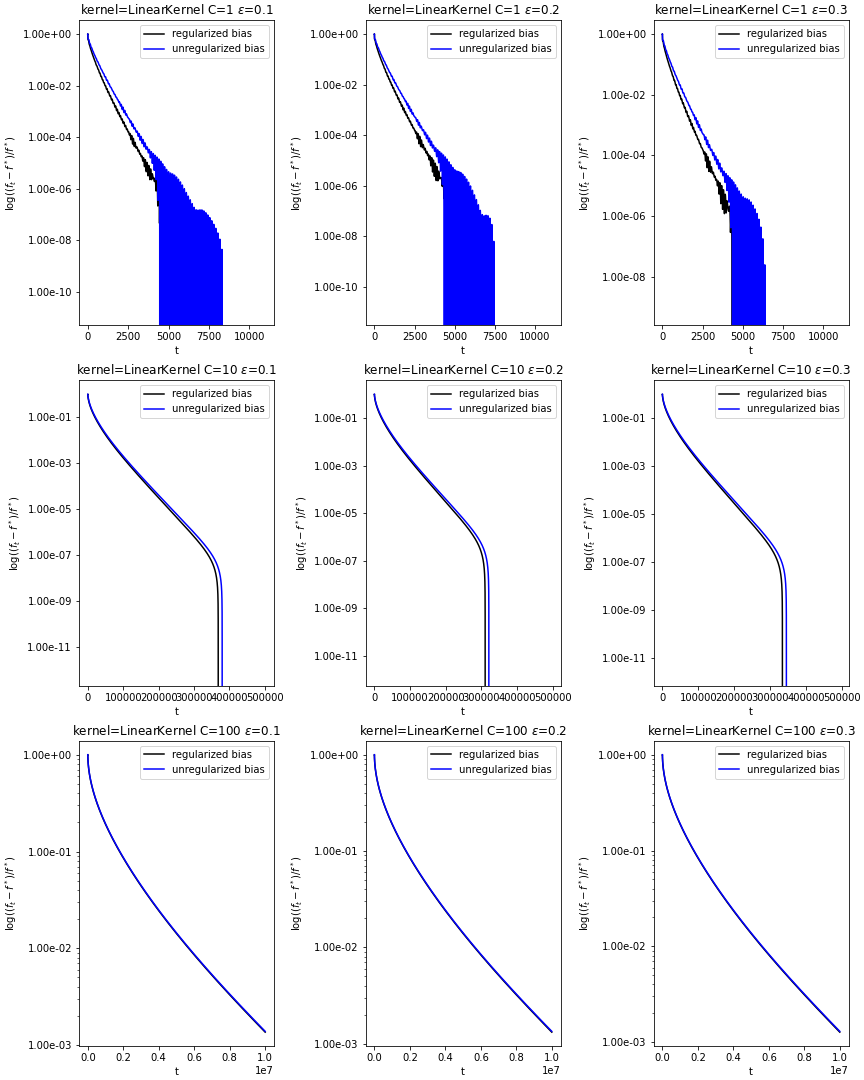
\includegraphics[scale=0.55]{img/linear_lagrangian_dual_l2_svr_loss_history}
	\caption{AdaGrad convergence for the Lagrangian Dual formulation of the linear $\protect \mathcal{L}_2$-SVR}
	\label{fig:linear_lagrangian_dual_l2_svr_loss_history}
\end{figure}

\paragraph{Nonlinear Dual formulations}

The experiments results shown in~\ref{nonlinear_lagrangian_dual_l2_svr_cv_results} are obtained with \emph{d} and \emph{r} hyperparameters both equal to 3 for the \emph{polynomial} kernel; \emph{gamma} is setted to \emph{`scale`} for both \emph{gaussian} and \emph{laplacian} kernels. The experiments results shown in~\ref{nonlinear_lagrangian_dual_l2_svr_cv_results} are obtained with $\alpha$, i.e., the \emph{learning rate} or \emph{step size}, setted to 1 for the \emph{AdaGrad} algorithm. Note that the \emph{unreg\_bias} and \emph{reg\_bias} duals refers to the augmented dual formulations~\eqref{eq:l2_svr_aug_lagrangian_dual} and~\eqref{eq:l2_svr_lb_aug_lagrangian_dual} respectively with $\rho$ equals to 1. The optimization process is stopped if the primal-dual weight vector does not change by at least $1\mathrm{e}{-6}$  between two consecutive iterations.

\begin{table}[H]
\centering
\caption{Lagrangian Dual nonlinear $\protect \mathcal{L}_2$-SVR results}
\label{nonlinear_lagrangian_dual_l2_svr_cv_results}
\begin{tabular}{llllrrrr}
\toprule
           &     &     &     &    fit\_time &        r2 &  n\_iter &  n\_sv \\
dual & kernel & C & epsilon &             &           &         &       \\
\midrule
reg\_bias & poly & 1   & 0.1 &   97.551234 &  0.981708 &  100000 &   100 \\
           &     &     & 0.2 &   99.213337 &  0.975801 &  100000 &    97 \\
           &     &     & 0.3 &   96.057328 &  0.948619 &  100000 &    96 \\
           &     & 10  & 0.1 &   96.669691 &  0.968303 &  100000 &    99 \\
           &     &     & 0.2 &   96.580167 &  0.967125 &  100000 &    99 \\
           &     &     & 0.3 &   97.984428 &  0.974149 &  100000 &    98 \\
           &     & 100 & 0.1 &   96.924278 &  0.965041 &  100000 &   100 \\
           &     &     & 0.2 &   98.486066 &  0.980911 &  100000 &    96 \\
           &     &     & 0.3 &   95.471666 &  0.903538 &  100000 &    94 \\
           & rbf & 1   & 0.1 &    9.849164 &  0.980790 &    8467 &    38 \\
           &     &     & 0.2 &   10.063439 &  0.945653 &    8563 &    28 \\
           &     &     & 0.3 &   10.447014 &  0.886380 &    8627 &    23 \\
           &     & 10  & 0.1 &   65.058718 &  0.988575 &   53056 &    22 \\
           &     &     & 0.2 &   45.359936 &  0.957657 &   36215 &    11 \\
           &     &     & 0.3 &   46.770068 &  0.900641 &   37412 &     8 \\
           &     & 100 & 0.1 &  122.264825 &  0.989799 &  100000 &    19 \\
           &     &     & 0.2 &  120.171495 &  0.966485 &  100000 &    10 \\
           &     &     & 0.3 &  122.602509 &  0.920652 &  100000 &     7 \\
unreg\_bias & poly & 1   & 0.1 &   96.043177 &  0.981739 &  100000 &    99 \\
           &     &     & 0.2 &   95.672288 &  0.976645 &  100000 &    91 \\
           &     &     & 0.3 &   96.231995 &  0.971742 &  100000 &    99 \\
           &     & 10  & 0.1 &   96.942310 &  0.968902 &  100000 &   100 \\
           &     &     & 0.2 &   97.522340 &  0.981894 &  100000 &   100 \\
           &     &     & 0.3 &   95.140821 &  0.800723 &  100000 &    95 \\
           &     & 100 & 0.1 &   96.468312 &  0.965794 &  100000 &   100 \\
           &     &     & 0.2 &   98.143747 &  0.977436 &  100000 &    96 \\
           &     &     & 0.3 &   95.971270 &  0.975918 &  100000 &    96 \\
           & rbf & 1   & 0.1 &   19.112700 &  0.980790 &   16609 &    38 \\
           &     &     & 0.2 &   19.546136 &  0.945647 &   16818 &    28 \\
           &     &     & 0.3 &   20.166675 &  0.886373 &   16970 &    23 \\
           &     & 10  & 0.1 &  121.256781 &  0.988575 &   99391 &    22 \\
           &     &     & 0.2 &   83.407763 &  0.957660 &   67123 &    11 \\
           &     &     & 0.3 &   87.705072 &  0.900795 &   69138 &     8 \\
           &     & 100 & 0.1 &  124.393783 &  0.989783 &  100000 &    19 \\
           &     &     & 0.2 &  119.844592 &  0.966486 &  100000 &    10 \\
           &     &     & 0.3 &  124.659568 &  0.920584 &  100000 &     7 \\
\bottomrule
\end{tabular}
\end{table}


The same considerations made for the previous linear \emph{Lagrangian dual} formulations are confirmed also in the nonlinearly separable case. In this setting, the complexity of the model coming with higher $C$ regularization hyperparameters and lower $\epsilon$ values pays a larger tradeoff in terms of the number of \emph{iterations} of the algorithm.

\begin{figure}[H]
	\centering
	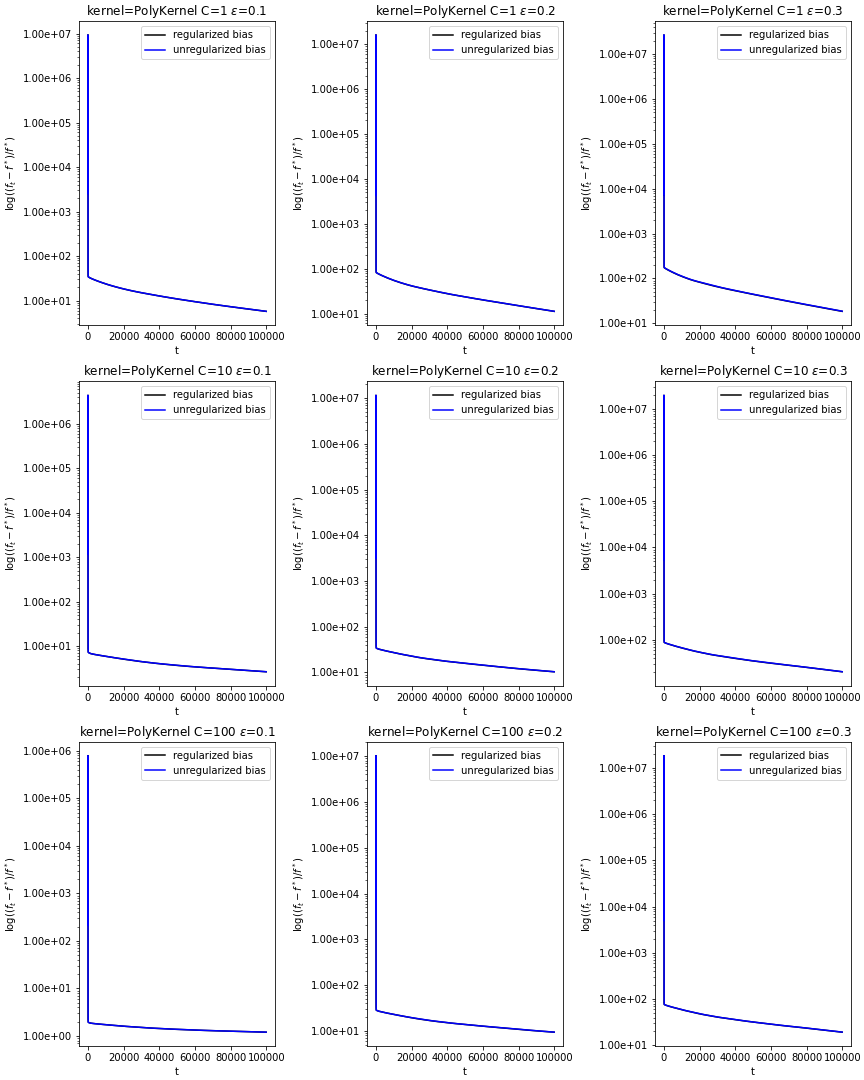
\includegraphics[scale=0.55]{img/laplacian_lagrangian_dual_l2_svr_loss_history}
	\caption{AdaGrad convergence for the Lagrangian Dual formulation of the Laplacian $\protect \mathcal{L}_2$-SVR}
	\label{fig:laplacian_lagrangian_dual_l2_svr_loss_history}
\end{figure}

\begin{figure}[H]
	\centering
	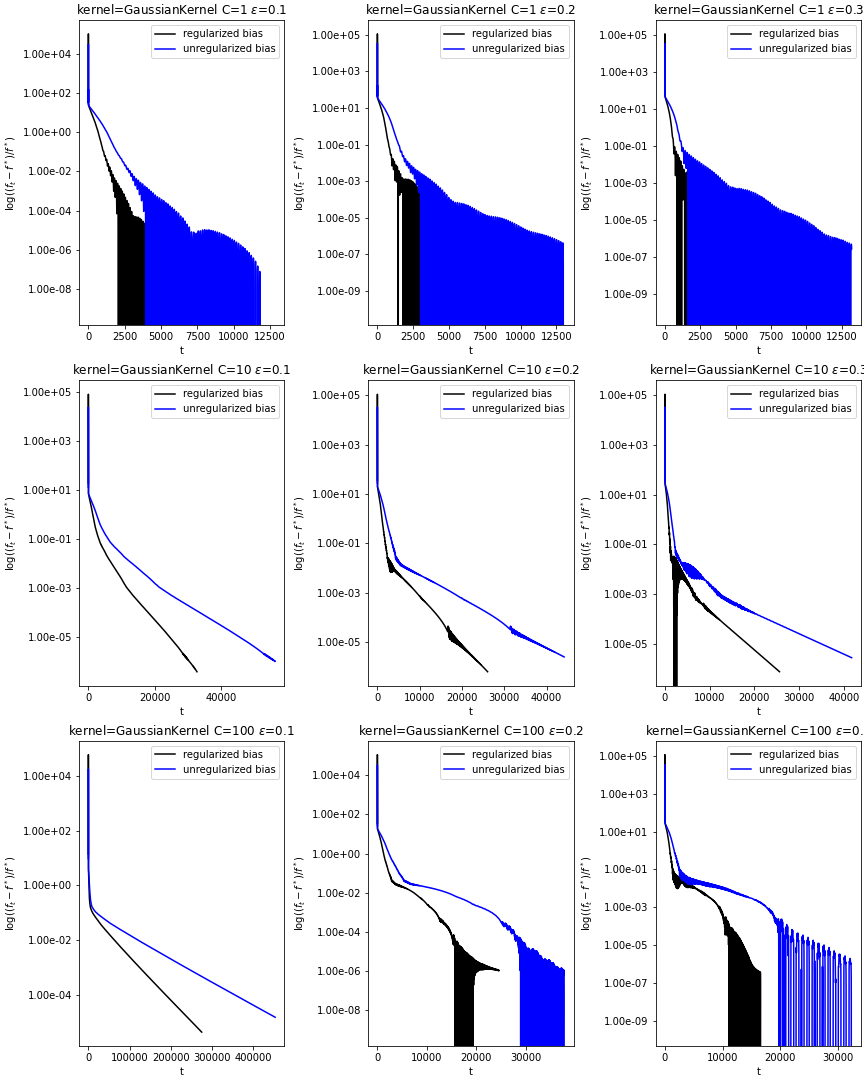
\includegraphics[scale=0.55]{img/gaussian_lagrangian_dual_l2_svr_loss_history}
	\caption{AdaGrad convergence for the Lagrangian Dual formulation of the Gaussian $\protect \mathcal{L}_2$-SVR}
	\label{fig:gaussian_lagrangian_dual_l2_svr_loss_history}
\end{figure}


\pagebreak

\section{Conclusions}

The actual \emph{convergence rates} of the \emph{primal} $\protect \mathcal{L}_1$-SVM formulations, i.e., the figures~\ref{fig:l1_svc_loss_history} and~\ref{fig:l1_svr_loss_history}, shows as they do not meet the theoretical expectations at the first line of the table~\ref{primal_svm_objectives_rates}. Both the \emph{Polyak} and the \emph{Nesterov} momentums provide a significant accelleration wrt the \emph{vanilla SGD} and they are quite comparable.

Conversely, the actual \emph{convergence rates} of the \emph{primal} $\protect \mathcal{L}_2$-SVM formulations, i.e., the figures~\ref{fig:l2_svc_loss_history} and~\ref{fig:l2_svr_loss_history}, shows as they do in part meet the theoretical expectations at the second line of the table~\ref{primal_svm_objectives_rates}. Despite the \emph{Nesterov} momentum provide a significant accelleration wrt the \emph{vanilla SGD} as expected, also the \emph{Polyak} momentm provide a quite comparable accelleration only reserved for the quadratic case according to the theoretical analysis.

In general, the complexity of the \emph{primal formulations} is dominated by the regularization parameter $C$: higher values allow the algorithms to converge faster.

\bigskip

The actual \emph{convergence rates} of the \emph{Lagrangian dual} formulations shows as they do not meet the theoretical expectations in the table~\ref{dual_svm_objectives_props}. The different \emph{convergence rate} is more highlighted in the linear case for lower regularization parameters $C$ but the situation is reversed as the latter grows. In the nonlinear settings, it depends on the kernel function, e.g., in the \emph{polynomial} case the convergence can become pathologically slower, meanwhile in the \emph{gaussian} or \emph{laplacian} case often it is better.

Moreover, from all the actual \emph{convergence rates} of the \emph{Lagrangian dual} formulations, it is evident that fitting the bias in an explicit way, i.e., by adding Lagrange multipliers to control the equality constraint, always causes slower converge of the \emph{AdaGrad} algorithm wrt the \emph{Lagrangian dual} of the problem where the bias term embedded into the Hessian matrix.

Unlike the \emph{primal formulations}, in the \emph{Lagrangian dual} case the complexity grows with the $C$ regularization parameter.

\bigskip

All the \emph{custom} implementations underperforms the others, i.e., \emph{liblinear}~\cite{fan2008liblinear}, \emph{libsvm}~\cite{chang2011libsvm} and \emph{cvxopt}~\cite{vandenberghe2010cvxopt} implementations, in terms of \emph{time} obviously in part due to the different core implementation languages, i.e., Python vs C, in part due to the different algorithm uses to solve the  optimization problem, e.g., the \emph{liblinear}~\cite{fan2008liblinear} implementation uses the \emph{Coordinate Gradient Descent} to sove the \emph{primal formulation} which minimizes one coordinate at a time.

Meanwhile, for what about the \emph{Wolfe dual} formulations, despite \emph{cvxopt}~\cite{vandenberghe2010cvxopt} underperforms the \emph{libsvm}~\cite{chang2011libsvm} implementation in terms of \emph{time}, since it is a general-purpose QP solver and it does not exploit the structure of the problem, the number of \emph{iterations} of the \emph{custom} SMO algorithm is always lower wrt that in \emph{libsvm}~\cite{chang2011libsvm}, probably due to the improvements described in~\cite{keerthi2001improvements, shevade1999improvements} for classification and regression respectively.

\bigskip

Finally, all the \emph{primal formulations} are suitable for potentially large linear training since the complexity of the model grows with the number of features or, more in general, when the number of examples $n$ is much larger than the number of features $m$, i.e., $n \gg m$.

Meanwhile, the \emph{dual formulations} are suitable in case the number of examples $n$ is less than the number of features $m$, i.e., $n < m$, since the complexity of the model is dominated by the number of examples. The \emph{Lagrangian} formulation never overperforms the \emph{Wolfe} one in our experiments, neither in terms of \emph{time} nor in terms of \emph{iterations}, but it is useful to highlight the complexity introduced by the dual formulation. Its training time complexity is more than quadratic with the number of samples which makes it hard to scale to large datasets. In this case, it could be useful to use the \emph{primal formulation} possibly after a nonlinear transformation of the instance vectors (if this should not be in the given space) using a low-rank kernel matrix approximation, i.e., Nyström, before training.

\pagebreak

\bibliographystyle{unsrt}
\bibliography{bibliography}

\end{document}
